% Options for packages loaded elsewhere
% Options for packages loaded elsewhere
\PassOptionsToPackage{unicode}{hyperref}
\PassOptionsToPackage{hyphens}{url}
\PassOptionsToPackage{dvipsnames,svgnames,x11names}{xcolor}
%
\documentclass[
  letterpaper,
  DIV=11,
  numbers=noendperiod]{scrartcl}
\usepackage{xcolor}
\usepackage[margin=1in]{geometry}
\usepackage{amsmath,amssymb}
\setcounter{secnumdepth}{5}
\usepackage{iftex}
\ifPDFTeX
  \usepackage[T1]{fontenc}
  \usepackage[utf8]{inputenc}
  \usepackage{textcomp} % provide euro and other symbols
\else % if luatex or xetex
  \usepackage{unicode-math} % this also loads fontspec
  \defaultfontfeatures{Scale=MatchLowercase}
  \defaultfontfeatures[\rmfamily]{Ligatures=TeX,Scale=1}
\fi
\usepackage{lmodern}
\ifPDFTeX\else
  % xetex/luatex font selection
  \setmainfont[]{Latin Modern Roman}
  \setsansfont[]{Latin Modern Sans}
  \setmonofont[]{Latin Modern Mono}
\fi
% Use upquote if available, for straight quotes in verbatim environments
\IfFileExists{upquote.sty}{\usepackage{upquote}}{}
\IfFileExists{microtype.sty}{% use microtype if available
  \usepackage[]{microtype}
  \UseMicrotypeSet[protrusion]{basicmath} % disable protrusion for tt fonts
}{}
\makeatletter
\@ifundefined{KOMAClassName}{% if non-KOMA class
  \IfFileExists{parskip.sty}{%
    \usepackage{parskip}
  }{% else
    \setlength{\parindent}{0pt}
    \setlength{\parskip}{6pt plus 2pt minus 1pt}}
}{% if KOMA class
  \KOMAoptions{parskip=half}}
\makeatother
% Make \paragraph and \subparagraph free-standing
\makeatletter
\ifx\paragraph\undefined\else
  \let\oldparagraph\paragraph
  \renewcommand{\paragraph}{
    \@ifstar
      \xxxParagraphStar
      \xxxParagraphNoStar
  }
  \newcommand{\xxxParagraphStar}[1]{\oldparagraph*{#1}\mbox{}}
  \newcommand{\xxxParagraphNoStar}[1]{\oldparagraph{#1}\mbox{}}
\fi
\ifx\subparagraph\undefined\else
  \let\oldsubparagraph\subparagraph
  \renewcommand{\subparagraph}{
    \@ifstar
      \xxxSubParagraphStar
      \xxxSubParagraphNoStar
  }
  \newcommand{\xxxSubParagraphStar}[1]{\oldsubparagraph*{#1}\mbox{}}
  \newcommand{\xxxSubParagraphNoStar}[1]{\oldsubparagraph{#1}\mbox{}}
\fi
\makeatother

\usepackage{color}
\usepackage{fancyvrb}
\newcommand{\VerbBar}{|}
\newcommand{\VERB}{\Verb[commandchars=\\\{\}]}
\DefineVerbatimEnvironment{Highlighting}{Verbatim}{commandchars=\\\{\}}
% Add ',fontsize=\small' for more characters per line
\usepackage{framed}
\definecolor{shadecolor}{RGB}{241,243,245}
\newenvironment{Shaded}{\begin{snugshade}}{\end{snugshade}}
\newcommand{\AlertTok}[1]{\textcolor[rgb]{0.68,0.00,0.00}{#1}}
\newcommand{\AnnotationTok}[1]{\textcolor[rgb]{0.37,0.37,0.37}{#1}}
\newcommand{\AttributeTok}[1]{\textcolor[rgb]{0.40,0.45,0.13}{#1}}
\newcommand{\BaseNTok}[1]{\textcolor[rgb]{0.68,0.00,0.00}{#1}}
\newcommand{\BuiltInTok}[1]{\textcolor[rgb]{0.00,0.23,0.31}{#1}}
\newcommand{\CharTok}[1]{\textcolor[rgb]{0.13,0.47,0.30}{#1}}
\newcommand{\CommentTok}[1]{\textcolor[rgb]{0.37,0.37,0.37}{#1}}
\newcommand{\CommentVarTok}[1]{\textcolor[rgb]{0.37,0.37,0.37}{\textit{#1}}}
\newcommand{\ConstantTok}[1]{\textcolor[rgb]{0.56,0.35,0.01}{#1}}
\newcommand{\ControlFlowTok}[1]{\textcolor[rgb]{0.00,0.23,0.31}{\textbf{#1}}}
\newcommand{\DataTypeTok}[1]{\textcolor[rgb]{0.68,0.00,0.00}{#1}}
\newcommand{\DecValTok}[1]{\textcolor[rgb]{0.68,0.00,0.00}{#1}}
\newcommand{\DocumentationTok}[1]{\textcolor[rgb]{0.37,0.37,0.37}{\textit{#1}}}
\newcommand{\ErrorTok}[1]{\textcolor[rgb]{0.68,0.00,0.00}{#1}}
\newcommand{\ExtensionTok}[1]{\textcolor[rgb]{0.00,0.23,0.31}{#1}}
\newcommand{\FloatTok}[1]{\textcolor[rgb]{0.68,0.00,0.00}{#1}}
\newcommand{\FunctionTok}[1]{\textcolor[rgb]{0.28,0.35,0.67}{#1}}
\newcommand{\ImportTok}[1]{\textcolor[rgb]{0.00,0.46,0.62}{#1}}
\newcommand{\InformationTok}[1]{\textcolor[rgb]{0.37,0.37,0.37}{#1}}
\newcommand{\KeywordTok}[1]{\textcolor[rgb]{0.00,0.23,0.31}{\textbf{#1}}}
\newcommand{\NormalTok}[1]{\textcolor[rgb]{0.00,0.23,0.31}{#1}}
\newcommand{\OperatorTok}[1]{\textcolor[rgb]{0.37,0.37,0.37}{#1}}
\newcommand{\OtherTok}[1]{\textcolor[rgb]{0.00,0.23,0.31}{#1}}
\newcommand{\PreprocessorTok}[1]{\textcolor[rgb]{0.68,0.00,0.00}{#1}}
\newcommand{\RegionMarkerTok}[1]{\textcolor[rgb]{0.00,0.23,0.31}{#1}}
\newcommand{\SpecialCharTok}[1]{\textcolor[rgb]{0.37,0.37,0.37}{#1}}
\newcommand{\SpecialStringTok}[1]{\textcolor[rgb]{0.13,0.47,0.30}{#1}}
\newcommand{\StringTok}[1]{\textcolor[rgb]{0.13,0.47,0.30}{#1}}
\newcommand{\VariableTok}[1]{\textcolor[rgb]{0.07,0.07,0.07}{#1}}
\newcommand{\VerbatimStringTok}[1]{\textcolor[rgb]{0.13,0.47,0.30}{#1}}
\newcommand{\WarningTok}[1]{\textcolor[rgb]{0.37,0.37,0.37}{\textit{#1}}}

\usepackage{longtable,booktabs,array}
\usepackage{multirow}
\usepackage{calc} % for calculating minipage widths
% Correct order of tables after \paragraph or \subparagraph
\usepackage{etoolbox}
\makeatletter
\patchcmd\longtable{\par}{\if@noskipsec\mbox{}\fi\par}{}{}
\makeatother
% Allow footnotes in longtable head/foot
\IfFileExists{footnotehyper.sty}{\usepackage{footnotehyper}}{\usepackage{footnote}}
\makesavenoteenv{longtable}
\usepackage{graphicx}
\makeatletter
\newsavebox\pandoc@box
\newcommand*\pandocbounded[1]{% scales image to fit in text height/width
  \sbox\pandoc@box{#1}%
  \Gscale@div\@tempa{\textheight}{\dimexpr\ht\pandoc@box+\dp\pandoc@box\relax}%
  \Gscale@div\@tempb{\linewidth}{\wd\pandoc@box}%
  \ifdim\@tempb\p@<\@tempa\p@\let\@tempa\@tempb\fi% select the smaller of both
  \ifdim\@tempa\p@<\p@\scalebox{\@tempa}{\usebox\pandoc@box}%
  \else\usebox{\pandoc@box}%
  \fi%
}
% Set default figure placement to htbp
\def\fps@figure{htbp}
\makeatother


% definitions for citeproc citations
\NewDocumentCommand\citeproctext{}{}
\NewDocumentCommand\citeproc{mm}{%
  \begingroup\def\citeproctext{#2}\cite{#1}\endgroup}
\makeatletter
 % allow citations to break across lines
 \let\@cite@ofmt\@firstofone
 % avoid brackets around text for \cite:
 \def\@biblabel#1{}
 \def\@cite#1#2{{#1\if@tempswa , #2\fi}}
\makeatother
\newlength{\cslhangindent}
\setlength{\cslhangindent}{1.5em}
\newlength{\csllabelwidth}
\setlength{\csllabelwidth}{3em}
\newenvironment{CSLReferences}[2] % #1 hanging-indent, #2 entry-spacing
 {\begin{list}{}{%
  \setlength{\itemindent}{0pt}
  \setlength{\leftmargin}{0pt}
  \setlength{\parsep}{0pt}
  % turn on hanging indent if param 1 is 1
  \ifodd #1
   \setlength{\leftmargin}{\cslhangindent}
   \setlength{\itemindent}{-1\cslhangindent}
  \fi
  % set entry spacing
  \setlength{\itemsep}{#2\baselineskip}}}
 {\end{list}}
\usepackage{calc}
\newcommand{\CSLBlock}[1]{\hfill\break\parbox[t]{\linewidth}{\strut\ignorespaces#1\strut}}
\newcommand{\CSLLeftMargin}[1]{\parbox[t]{\csllabelwidth}{\strut#1\strut}}
\newcommand{\CSLRightInline}[1]{\parbox[t]{\linewidth - \csllabelwidth}{\strut#1\strut}}
\newcommand{\CSLIndent}[1]{\hspace{\cslhangindent}#1}



\setlength{\emergencystretch}{3em} % prevent overfull lines

\providecommand{\tightlist}{%
  \setlength{\itemsep}{0pt}\setlength{\parskip}{0pt}}



 


% Colors and section/title styling using KOMA-Script interfaces
\usepackage{xcolor}
\definecolor{sectionblue}{HTML}{2563eb}

% KOMA: headings and title/subtitle colors
\setkomafont{title}{\color{sectionblue}\bfseries\Huge}
\setkomafont{subtitle}{\color{sectionblue}\large}
\setkomafont{section}{\color{sectionblue}\bfseries\Large}
\setkomafont{subsection}{\color{sectionblue}\bfseries\large}

% Code block styling via Shaded redefinition
\usepackage{tcolorbox}
\tcbuselibrary{skins,breakable}
\definecolor{codebg}{HTML}{F0F8FF}
\renewenvironment{Shaded}{%
  \begin{tcolorbox}[%
    enhanced,%
    colback=codebg,%
    colframe=codebg,%
    borderline west={3pt}{0pt}{sectionblue},%
    fontupper=\small\ttfamily,% reduce font size and force monospace for code
    boxrule=0pt,%
    arc=0pt,%
    boxsep=5pt,%
    left=2mm,%
    right=2mm,%
    top=2mm,%
    bottom=2mm% 
  ]% 
}{%
  \end{tcolorbox}%
}
\KOMAoption{captions}{tableheading}
\makeatletter
\@ifpackageloaded{caption}{}{\usepackage{caption}}
\AtBeginDocument{%
\ifdefined\contentsname
  \renewcommand*\contentsname{Table of contents}
\else
  \newcommand\contentsname{Table of contents}
\fi
\ifdefined\listfigurename
  \renewcommand*\listfigurename{List of Figures}
\else
  \newcommand\listfigurename{List of Figures}
\fi
\ifdefined\listtablename
  \renewcommand*\listtablename{List of Tables}
\else
  \newcommand\listtablename{List of Tables}
\fi
\ifdefined\figurename
  \renewcommand*\figurename{Figure}
\else
  \newcommand\figurename{Figure}
\fi
\ifdefined\tablename
  \renewcommand*\tablename{Table}
\else
  \newcommand\tablename{Table}
\fi
}
\@ifpackageloaded{float}{}{\usepackage{float}}
\floatstyle{ruled}
\@ifundefined{c@chapter}{\newfloat{codelisting}{h}{lop}}{\newfloat{codelisting}{h}{lop}[chapter]}
\floatname{codelisting}{Listing}
\newcommand*\listoflistings{\listof{codelisting}{List of Listings}}
\makeatother
\makeatletter
\makeatother
\makeatletter
\@ifpackageloaded{caption}{}{\usepackage{caption}}
\@ifpackageloaded{subcaption}{}{\usepackage{subcaption}}
\makeatother
\usepackage{bookmark}
\IfFileExists{xurl.sty}{\usepackage{xurl}}{} % add URL line breaks if available
\urlstyle{same}
\hypersetup{
  pdftitle={Discovering Drift Patterns in Sensor Arrays},
  colorlinks=true,
  linkcolor={blue},
  filecolor={Maroon},
  citecolor={Blue},
  urlcolor={Blue},
  pdfcreator={LaTeX via pandoc}}


\title{Discovering Drift Patterns in Sensor Arrays}
\usepackage{etoolbox}
\makeatletter
\providecommand{\subtitle}[1]{% add subtitle to \maketitle
  \apptocmd{\@title}{\par {\large #1 \par}}{}{}
}
\makeatother
\subtitle{A Principal Component Perspective on Chemical Signature
Stability}
\author{}
\date{}
\begin{document}
\maketitle

\renewcommand*\contentsname{Table of contents}
{
\hypersetup{linkcolor=}
\setcounter{tocdepth}{3}
\tableofcontents
}

\section{A Principal Component Perspective on Chemical Signature
Stability}\label{a-principal-component-perspective-on-chemical-signature-stability}

This notebook investigates sensor drift in gas sensor arrays through an
unsupervised lens, discovering stable geometric structures and drift
patterns without applying any corrections.

\section{Setup and Data Loading}\label{setup-and-data-loading}

\begin{Shaded}
\begin{Highlighting}[]
\ImportTok{import}\NormalTok{ numpy }\ImportTok{as}\NormalTok{ np}
\ImportTok{import}\NormalTok{ pandas }\ImportTok{as}\NormalTok{ pd}
\ImportTok{import}\NormalTok{ matplotlib.pyplot }\ImportTok{as}\NormalTok{ plt}
\ImportTok{import}\NormalTok{ seaborn }\ImportTok{as}\NormalTok{ sns}
\ImportTok{from}\NormalTok{ pathlib }\ImportTok{import}\NormalTok{ Path}
\ImportTok{from}\NormalTok{ IPython.display }\ImportTok{import}\NormalTok{ display}
\ImportTok{from}\NormalTok{ scipy.spatial.distance }\ImportTok{import}\NormalTok{ cdist, pdist}
\ImportTok{from}\NormalTok{ scipy.optimize }\ImportTok{import}\NormalTok{ linear\_sum\_assignment}
\ImportTok{from}\NormalTok{ scipy.stats }\ImportTok{import}\NormalTok{ spearmanr}
\ImportTok{from}\NormalTok{ scipy.linalg }\ImportTok{import}\NormalTok{ orthogonal\_procrustes, subspace\_angles}
\ImportTok{from}\NormalTok{ sklearn.decomposition }\ImportTok{import}\NormalTok{ PCA}
\ImportTok{from}\NormalTok{ sklearn.preprocessing }\ImportTok{import}\NormalTok{ StandardScaler}
\ImportTok{from}\NormalTok{ sklearn.cluster }\ImportTok{import}\NormalTok{ KMeans}
\ImportTok{from}\NormalTok{ sklearn.metrics }\ImportTok{import}\NormalTok{ silhouette\_score, davies\_bouldin\_score}

\CommentTok{\# Set visualization style}
\NormalTok{sns.set\_context(}\StringTok{"notebook"}\NormalTok{)}
\NormalTok{plt.style.use(}\StringTok{\textquotesingle{}seaborn{-}v0\_8{-}darkgrid\textquotesingle{}}\NormalTok{)}

\KeywordTok{def}\NormalTok{ \_resolve\_data\_path() }\OperatorTok{{-}\textgreater{}}\NormalTok{ Path:}
    \CommentTok{"""Return a path to the processed sensor CSV regardless of launch directory."""}
\NormalTok{    candidates }\OperatorTok{=}\NormalTok{ [}
\NormalTok{        Path.cwd() }\OperatorTok{/} \StringTok{"data"} \OperatorTok{/} \StringTok{"processed"} \OperatorTok{/} \StringTok{"sensor\_data.csv"}\NormalTok{,}
\NormalTok{        Path.cwd().parent }\OperatorTok{/} \StringTok{"data"} \OperatorTok{/} \StringTok{"processed"} \OperatorTok{/} \StringTok{"sensor\_data.csv"}\NormalTok{,}
\NormalTok{    ]}
    \ControlFlowTok{for}\NormalTok{ candidate }\KeywordTok{in}\NormalTok{ candidates:}
        \ControlFlowTok{if}\NormalTok{ candidate.exists():}
            \ControlFlowTok{return}\NormalTok{ candidate}
\NormalTok{    checked }\OperatorTok{=} \StringTok{"}\CharTok{\textbackslash{}n}\StringTok{"}\NormalTok{.join(}\BuiltInTok{str}\NormalTok{(p) }\ControlFlowTok{for}\NormalTok{ p }\KeywordTok{in}\NormalTok{ candidates)}
    \ControlFlowTok{raise} \PreprocessorTok{FileNotFoundError}\NormalTok{(}\SpecialStringTok{f"Unable to locate sensor\_data.csv. Checked: }\CharTok{\textbackslash{}n}\SpecialCharTok{\{}\NormalTok{checked}\SpecialCharTok{\}}\SpecialStringTok{"}\NormalTok{)}

\CommentTok{\# Load and prepare data}
\NormalTok{csv\_path }\OperatorTok{=}\NormalTok{ \_resolve\_data\_path()}
\NormalTok{df }\OperatorTok{=}\NormalTok{ pd.read\_csv(csv\_path)}
\ControlFlowTok{if}\NormalTok{ df[}\StringTok{"batch"}\NormalTok{].dtype.kind }\KeywordTok{not} \KeywordTok{in} \StringTok{"iu"}\NormalTok{:}
\NormalTok{    df[}\StringTok{"batch"}\NormalTok{] }\OperatorTok{=}\NormalTok{ df[}\StringTok{"batch"}\NormalTok{].astype(}\BuiltInTok{int}\NormalTok{)}
\NormalTok{df }\OperatorTok{=}\NormalTok{ df.sort\_values(}\StringTok{"batch"}\NormalTok{).reset\_index(drop}\OperatorTok{=}\VariableTok{True}\NormalTok{)}

\CommentTok{\# Extract sensor columns and batches}
\NormalTok{sensor\_cols }\OperatorTok{=}\NormalTok{ [col }\ControlFlowTok{for}\NormalTok{ col }\KeywordTok{in}\NormalTok{ df.columns }\ControlFlowTok{if}\NormalTok{ col.startswith(}\StringTok{"S"}\NormalTok{)]}
\NormalTok{batches }\OperatorTok{=} \BuiltInTok{sorted}\NormalTok{(df[}\StringTok{"batch"}\NormalTok{].unique())}

\CommentTok{\# Standardize sensor readings}
\NormalTok{scaler }\OperatorTok{=}\NormalTok{ StandardScaler()}
\NormalTok{X\_scaled }\OperatorTok{=}\NormalTok{ scaler.fit\_transform(df[sensor\_cols])}

\BuiltInTok{print}\NormalTok{(}\SpecialStringTok{f"Data loaded: }\SpecialCharTok{\{}\NormalTok{X\_scaled}\SpecialCharTok{.}\NormalTok{shape[}\DecValTok{0}\NormalTok{]}\SpecialCharTok{\}}\SpecialStringTok{ samples, }\SpecialCharTok{\{}\NormalTok{X\_scaled}\SpecialCharTok{.}\NormalTok{shape[}\DecValTok{1}\NormalTok{]}\SpecialCharTok{\}}\SpecialStringTok{ sensors, }\SpecialCharTok{\{}\BuiltInTok{len}\NormalTok{(batches)}\SpecialCharTok{\}}\SpecialStringTok{ batches"}\NormalTok{)}
\BuiltInTok{print}\NormalTok{(}\SpecialStringTok{f"Time span: Batch }\SpecialCharTok{\{}\NormalTok{batches[}\DecValTok{0}\NormalTok{]}\SpecialCharTok{\}}\SpecialStringTok{ to Batch }\SpecialCharTok{\{}\NormalTok{batches[}\OperatorTok{{-}}\DecValTok{1}\NormalTok{]}\SpecialCharTok{\}}\SpecialStringTok{"}\NormalTok{)}
\end{Highlighting}
\end{Shaded}

\begin{verbatim}
Data loaded: 13910 samples, 128 sensors, 10 batches
Time span: Batch 1 to Batch 10
\end{verbatim}

\section{Section 1: Dimensionality
Discovery}\label{section-1-dimensionality-discovery}

First, we investigate the intrinsic dimensionality of the sensor array
data through eigenvalue spectrum analysis.

\begin{Shaded}
\begin{Highlighting}[]
\CommentTok{\# Perform global PCA}
\NormalTok{pca\_global }\OperatorTok{=}\NormalTok{ PCA(n\_components}\OperatorTok{=}\DecValTok{30}\NormalTok{, svd\_solver}\OperatorTok{=}\StringTok{\textquotesingle{}full\textquotesingle{}}\NormalTok{)}
\NormalTok{scores\_global }\OperatorTok{=}\NormalTok{ pca\_global.fit\_transform(X\_scaled)}

\CommentTok{\# Create explained variance dataframe}
\NormalTok{explained\_df }\OperatorTok{=}\NormalTok{ pd.DataFrame(\{}
    \StringTok{"component"}\NormalTok{: np.arange(}\DecValTok{1}\NormalTok{, pca\_global.n\_components\_ }\OperatorTok{+} \DecValTok{1}\NormalTok{),}
    \StringTok{"explained\_variance\_ratio"}\NormalTok{: pca\_global.explained\_variance\_ratio\_,}
    \StringTok{"eigenvalue"}\NormalTok{: pca\_global.explained\_variance\_}
\NormalTok{\})}
\NormalTok{explained\_df[}\StringTok{"cumulative\_variance"}\NormalTok{] }\OperatorTok{=}\NormalTok{ explained\_df[}\StringTok{"explained\_variance\_ratio"}\NormalTok{].cumsum()}

\BuiltInTok{print}\NormalTok{(}\StringTok{"}\CharTok{\textbackslash{}n}\StringTok{===== DIMENSIONALITY ANALYSIS ====="}\NormalTok{)}
\BuiltInTok{print}\NormalTok{(}\StringTok{"}\CharTok{\textbackslash{}n}\StringTok{Variance explained by principal components:"}\NormalTok{)}
\NormalTok{display(explained\_df.head(}\DecValTok{12}\NormalTok{))}

\CommentTok{\# Visualization}
\NormalTok{fig, axes }\OperatorTok{=}\NormalTok{ plt.subplots(}\DecValTok{1}\NormalTok{, }\DecValTok{3}\NormalTok{, figsize}\OperatorTok{=}\NormalTok{(}\DecValTok{15}\NormalTok{, }\DecValTok{4}\NormalTok{))}

\CommentTok{\# Scree plot}
\NormalTok{axes[}\DecValTok{0}\NormalTok{].plot(explained\_df[}\StringTok{\textquotesingle{}component\textquotesingle{}}\NormalTok{], explained\_df[}\StringTok{\textquotesingle{}eigenvalue\textquotesingle{}}\NormalTok{], }\StringTok{\textquotesingle{}o{-}\textquotesingle{}}\NormalTok{)}
\NormalTok{axes[}\DecValTok{0}\NormalTok{].axhline(y}\OperatorTok{=}\DecValTok{1}\NormalTok{, color}\OperatorTok{=}\StringTok{\textquotesingle{}r\textquotesingle{}}\NormalTok{, linestyle}\OperatorTok{=}\StringTok{\textquotesingle{}{-}{-}\textquotesingle{}}\NormalTok{, alpha}\OperatorTok{=}\FloatTok{0.5}\NormalTok{, label}\OperatorTok{=}\StringTok{\textquotesingle{}Kaiser criterion\textquotesingle{}}\NormalTok{)}
\NormalTok{axes[}\DecValTok{0}\NormalTok{].set\_xlabel(}\StringTok{\textquotesingle{}Principal Component\textquotesingle{}}\NormalTok{)}
\NormalTok{axes[}\DecValTok{0}\NormalTok{].set\_ylabel(}\StringTok{\textquotesingle{}Eigenvalue\textquotesingle{}}\NormalTok{)}
\NormalTok{axes[}\DecValTok{0}\NormalTok{].set\_title(}\StringTok{\textquotesingle{}Scree Plot\textquotesingle{}}\NormalTok{)}
\NormalTok{axes[}\DecValTok{0}\NormalTok{].legend()}
\NormalTok{axes[}\DecValTok{0}\NormalTok{].grid(}\VariableTok{True}\NormalTok{, alpha}\OperatorTok{=}\FloatTok{0.3}\NormalTok{)}

\CommentTok{\# Explained variance ratio}
\NormalTok{axes[}\DecValTok{1}\NormalTok{].bar(explained\_df[}\StringTok{\textquotesingle{}component\textquotesingle{}}\NormalTok{][:}\DecValTok{10}\NormalTok{], explained\_df[}\StringTok{\textquotesingle{}explained\_variance\_ratio\textquotesingle{}}\NormalTok{][:}\DecValTok{10}\NormalTok{])}
\NormalTok{axes[}\DecValTok{1}\NormalTok{].set\_xlabel(}\StringTok{\textquotesingle{}Principal Component\textquotesingle{}}\NormalTok{)}
\NormalTok{axes[}\DecValTok{1}\NormalTok{].set\_ylabel(}\StringTok{\textquotesingle{}Explained Variance Ratio\textquotesingle{}}\NormalTok{)}
\NormalTok{axes[}\DecValTok{1}\NormalTok{].set\_title(}\StringTok{\textquotesingle{}Variance Contribution per Component\textquotesingle{}}\NormalTok{)}
\NormalTok{axes[}\DecValTok{1}\NormalTok{].grid(}\VariableTok{True}\NormalTok{, alpha}\OperatorTok{=}\FloatTok{0.3}\NormalTok{)}

\CommentTok{\# Cumulative variance}
\NormalTok{axes[}\DecValTok{2}\NormalTok{].plot(explained\_df[}\StringTok{\textquotesingle{}component\textquotesingle{}}\NormalTok{], explained\_df[}\StringTok{\textquotesingle{}cumulative\_variance\textquotesingle{}}\NormalTok{], }\StringTok{\textquotesingle{}o{-}\textquotesingle{}}\NormalTok{)}
\NormalTok{axes[}\DecValTok{2}\NormalTok{].axhline(y}\OperatorTok{=}\FloatTok{0.95}\NormalTok{, color}\OperatorTok{=}\StringTok{\textquotesingle{}r\textquotesingle{}}\NormalTok{, linestyle}\OperatorTok{=}\StringTok{\textquotesingle{}{-}{-}\textquotesingle{}}\NormalTok{, alpha}\OperatorTok{=}\FloatTok{0.5}\NormalTok{, label}\OperatorTok{=}\StringTok{\textquotesingle{}95\% threshold\textquotesingle{}}\NormalTok{)}
\NormalTok{axes[}\DecValTok{2}\NormalTok{].axhline(y}\OperatorTok{=}\FloatTok{0.90}\NormalTok{, color}\OperatorTok{=}\StringTok{\textquotesingle{}orange\textquotesingle{}}\NormalTok{, linestyle}\OperatorTok{=}\StringTok{\textquotesingle{}{-}{-}\textquotesingle{}}\NormalTok{, alpha}\OperatorTok{=}\FloatTok{0.5}\NormalTok{, label}\OperatorTok{=}\StringTok{\textquotesingle{}90\% threshold\textquotesingle{}}\NormalTok{)}
\NormalTok{axes[}\DecValTok{2}\NormalTok{].set\_xlabel(}\StringTok{\textquotesingle{}Principal Component\textquotesingle{}}\NormalTok{)}
\NormalTok{axes[}\DecValTok{2}\NormalTok{].set\_ylabel(}\StringTok{\textquotesingle{}Cumulative Explained Variance\textquotesingle{}}\NormalTok{)}
\NormalTok{axes[}\DecValTok{2}\NormalTok{].set\_title(}\StringTok{\textquotesingle{}Cumulative Variance Explained\textquotesingle{}}\NormalTok{)}
\NormalTok{axes[}\DecValTok{2}\NormalTok{].legend()}
\NormalTok{axes[}\DecValTok{2}\NormalTok{].grid(}\VariableTok{True}\NormalTok{, alpha}\OperatorTok{=}\FloatTok{0.3}\NormalTok{)}

\NormalTok{plt.tight\_layout()}
\NormalTok{plt.show()}

\CommentTok{\# Key findings}
\NormalTok{n\_95 }\OperatorTok{=}\NormalTok{ (explained\_df[}\StringTok{\textquotesingle{}cumulative\_variance\textquotesingle{}}\NormalTok{] }\OperatorTok{\textgreater{}=} \FloatTok{0.95}\NormalTok{).idxmax() }\OperatorTok{+} \DecValTok{1}
\NormalTok{n\_90 }\OperatorTok{=}\NormalTok{ (explained\_df[}\StringTok{\textquotesingle{}cumulative\_variance\textquotesingle{}}\NormalTok{] }\OperatorTok{\textgreater{}=} \FloatTok{0.90}\NormalTok{).idxmax() }\OperatorTok{+} \DecValTok{1}
\BuiltInTok{print}\NormalTok{(}\SpecialStringTok{f"}\CharTok{\textbackslash{}n}\SpecialStringTok{Key Findings:"}\NormalTok{)}
\BuiltInTok{print}\NormalTok{(}\SpecialStringTok{f"{-} }\SpecialCharTok{\{}\NormalTok{n\_90}\SpecialCharTok{\}}\SpecialStringTok{ components explain 90\% of variance"}\NormalTok{)}
\BuiltInTok{print}\NormalTok{(}\SpecialStringTok{f"{-} }\SpecialCharTok{\{}\NormalTok{n\_95}\SpecialCharTok{\}}\SpecialStringTok{ components explain 95\% of variance"}\NormalTok{)}
\BuiltInTok{print}\NormalTok{(}\SpecialStringTok{f"{-} Conclusion: Dataset lives in \textasciitilde{}}\SpecialCharTok{\{}\NormalTok{n\_90}\SpecialCharTok{\}}\SpecialStringTok{D subspace, not 128D"}\NormalTok{)}
\end{Highlighting}
\end{Shaded}

\begin{verbatim}

===== DIMENSIONALITY ANALYSIS =====

Variance explained by principal components:
\end{verbatim}

\begin{longtable}[]{@{}lllll@{}}
\toprule\noalign{}
& component & explained\_variance\_ratio & eigenvalue &
cumulative\_variance \\
\midrule\noalign{}
\endhead
\bottomrule\noalign{}
\endlastfoot
0 & 1 & 0.535151 & 68.504298 & 0.535151 \\
1 & 2 & 0.150401 & 19.252659 & 0.685552 \\
2 & 3 & 0.060458 & 7.739124 & 0.746009 \\
3 & 4 & 0.050850 & 6.509256 & 0.796859 \\
4 & 5 & 0.035277 & 4.515747 & 0.832136 \\
5 & 6 & 0.029060 & 3.719978 & 0.861196 \\
6 & 7 & 0.023333 & 2.986861 & 0.884530 \\
7 & 8 & 0.015695 & 2.009168 & 0.900225 \\
8 & 9 & 0.014492 & 1.855114 & 0.914717 \\
9 & 10 & 0.011713 & 1.499318 & 0.926430 \\
10 & 11 & 0.010263 & 1.313760 & 0.936693 \\
11 & 12 & 0.008979 & 1.149364 & 0.945671 \\
\end{longtable}

\pandocbounded{\includegraphics[keepaspectratio]{PCA-Drift-Investigations-Revised_files/figure-pdf/cell-3-output-3.png}}

\begin{verbatim}

Key Findings:
- 8 components explain 90% of variance
- 13 components explain 95% of variance
- Conclusion: Dataset lives in ~8D subspace, not 128D
\end{verbatim}

\section{Section 2: Principal Component Stability
Analysis}\label{section-2-principal-component-stability-analysis}

We now analyze how stable the principal components are across batches by
computing principal angles between subspaces.

\begin{Shaded}
\begin{Highlighting}[]
\CommentTok{\# CRITICAL FIX: Measure actual drift in global PC space, not algorithmic variability}
\CommentTok{\# Computing separate PCAs per batch conflates data drift with PCA instability}
\CommentTok{\# Instead, we measure how data distributions shift in a consistent coordinate system}

\BuiltInTok{print}\NormalTok{(}\StringTok{"Analyzing stability in global PC space (consistent coordinate system)..."}\NormalTok{)}

\CommentTok{\# Use global PCA scores for all batches (already computed in Section 1)}
\NormalTok{n\_pcs }\OperatorTok{=} \DecValTok{10}
\NormalTok{global\_scores\_subset }\OperatorTok{=}\NormalTok{ scores\_global[:, :n\_pcs]}

\CommentTok{\# Reference batch for comparison}
\NormalTok{reference\_batch }\OperatorTok{=}\NormalTok{ batches[}\DecValTok{0}\NormalTok{]}
\NormalTok{ref\_mask }\OperatorTok{=}\NormalTok{ df[}\StringTok{\textquotesingle{}batch\textquotesingle{}}\NormalTok{] }\OperatorTok{==}\NormalTok{ reference\_batch}
\NormalTok{ref\_centroid }\OperatorTok{=}\NormalTok{ global\_scores\_subset[ref\_mask].mean(axis}\OperatorTok{=}\DecValTok{0}\NormalTok{)}
\NormalTok{ref\_cov }\OperatorTok{=}\NormalTok{ np.cov(global\_scores\_subset[ref\_mask].T)}

\CommentTok{\# Measure stability metrics for each batch}
\NormalTok{stability\_metrics }\OperatorTok{=}\NormalTok{ []}

\ControlFlowTok{for}\NormalTok{ batch }\KeywordTok{in}\NormalTok{ batches:}
\NormalTok{    mask }\OperatorTok{=}\NormalTok{ df[}\StringTok{\textquotesingle{}batch\textquotesingle{}}\NormalTok{] }\OperatorTok{==}\NormalTok{ batch}
\NormalTok{    batch\_scores }\OperatorTok{=}\NormalTok{ global\_scores\_subset[mask]}
\NormalTok{    batch\_centroid }\OperatorTok{=}\NormalTok{ batch\_scores.mean(axis}\OperatorTok{=}\DecValTok{0}\NormalTok{)}
\NormalTok{    batch\_cov }\OperatorTok{=}\NormalTok{ np.cov(batch\_scores.T)}
    
    \CommentTok{\# Measure centroid shift per PC}
\NormalTok{    centroid\_shifts }\OperatorTok{=}\NormalTok{ batch\_centroid }\OperatorTok{{-}}\NormalTok{ ref\_centroid}
    
    \CommentTok{\# Measure covariance change (stability of variance structure)}
\NormalTok{    cov\_distance }\OperatorTok{=}\NormalTok{ np.linalg.norm(batch\_cov }\OperatorTok{{-}}\NormalTok{ ref\_cov, }\StringTok{\textquotesingle{}fro\textquotesingle{}}\NormalTok{)}
    
    \CommentTok{\# Store metrics for each PC}
    \ControlFlowTok{for}\NormalTok{ pc\_idx }\KeywordTok{in} \BuiltInTok{range}\NormalTok{(n\_pcs):}
\NormalTok{        stability\_metrics.append(\{}
            \StringTok{\textquotesingle{}batch\textquotesingle{}}\NormalTok{: batch,}
            \StringTok{\textquotesingle{}PC\textquotesingle{}}\NormalTok{: pc\_idx }\OperatorTok{+} \DecValTok{1}\NormalTok{,}
            \StringTok{\textquotesingle{}centroid\_shift\textquotesingle{}}\NormalTok{: }\BuiltInTok{abs}\NormalTok{(centroid\_shifts[pc\_idx]),}
            \StringTok{\textquotesingle{}centroid\_shift\_signed\textquotesingle{}}\NormalTok{: centroid\_shifts[pc\_idx],}
            \StringTok{\textquotesingle{}variance\_explained\textquotesingle{}}\NormalTok{: pca\_global.explained\_variance\_ratio\_[pc\_idx],}
            \StringTok{\textquotesingle{}cov\_distance\textquotesingle{}}\NormalTok{: cov\_distance }\ControlFlowTok{if}\NormalTok{ batch }\OperatorTok{!=}\NormalTok{ reference\_batch }\ControlFlowTok{else} \DecValTok{0}
\NormalTok{        \})}

\NormalTok{stability\_df }\OperatorTok{=}\NormalTok{ pd.DataFrame(stability\_metrics)}

\BuiltInTok{print}\NormalTok{(}\StringTok{"}\CharTok{\textbackslash{}n}\StringTok{===== PRINCIPAL COMPONENT STABILITY ANALYSIS ====="}\NormalTok{)}
\BuiltInTok{print}\NormalTok{(}\StringTok{"}\CharTok{\textbackslash{}n}\StringTok{Measuring actual data drift in global PC space (no correction applied)"}\NormalTok{)}

\CommentTok{\# Visualization}
\NormalTok{fig, axes }\OperatorTok{=}\NormalTok{ plt.subplots(}\DecValTok{2}\NormalTok{, }\DecValTok{3}\NormalTok{, figsize}\OperatorTok{=}\NormalTok{(}\DecValTok{18}\NormalTok{, }\DecValTok{10}\NormalTok{))}

\CommentTok{\# 1. Centroid shifts over time}
\NormalTok{pivot\_shifts }\OperatorTok{=}\NormalTok{ stability\_df.pivot(index}\OperatorTok{=}\StringTok{\textquotesingle{}batch\textquotesingle{}}\NormalTok{, columns}\OperatorTok{=}\StringTok{\textquotesingle{}PC\textquotesingle{}}\NormalTok{, values}\OperatorTok{=}\StringTok{\textquotesingle{}centroid\_shift\textquotesingle{}}\NormalTok{)}
\ControlFlowTok{for}\NormalTok{ pc }\KeywordTok{in} \BuiltInTok{range}\NormalTok{(}\DecValTok{1}\NormalTok{, }\BuiltInTok{min}\NormalTok{(}\DecValTok{6}\NormalTok{, n\_pcs}\OperatorTok{+}\DecValTok{1}\NormalTok{)):}
\NormalTok{    axes[}\DecValTok{0}\NormalTok{, }\DecValTok{0}\NormalTok{].plot(pivot\_shifts.index, pivot\_shifts[pc], marker}\OperatorTok{=}\StringTok{\textquotesingle{}o\textquotesingle{}}\NormalTok{, label}\OperatorTok{=}\SpecialStringTok{f\textquotesingle{}PC}\SpecialCharTok{\{}\NormalTok{pc}\SpecialCharTok{\}}\SpecialStringTok{\textquotesingle{}}\NormalTok{, linewidth}\OperatorTok{=}\DecValTok{2}\NormalTok{)}
\NormalTok{axes[}\DecValTok{0}\NormalTok{, }\DecValTok{0}\NormalTok{].set\_xlabel(}\StringTok{\textquotesingle{}Batch\textquotesingle{}}\NormalTok{)}
\NormalTok{axes[}\DecValTok{0}\NormalTok{, }\DecValTok{0}\NormalTok{].set\_ylabel(}\StringTok{\textquotesingle{}Absolute Centroid Shift\textquotesingle{}}\NormalTok{)}
\NormalTok{axes[}\DecValTok{0}\NormalTok{, }\DecValTok{0}\NormalTok{].set\_title(}\StringTok{\textquotesingle{}Centroid Drift Magnitude per PC\textquotesingle{}}\NormalTok{)}
\NormalTok{axes[}\DecValTok{0}\NormalTok{, }\DecValTok{0}\NormalTok{].legend()}
\NormalTok{axes[}\DecValTok{0}\NormalTok{, }\DecValTok{0}\NormalTok{].grid(}\VariableTok{True}\NormalTok{, alpha}\OperatorTok{=}\FloatTok{0.3}\NormalTok{)}

\CommentTok{\# 2. Cumulative drift per PC}
\NormalTok{cumulative\_drift\_by\_pc }\OperatorTok{=}\NormalTok{ []}
\ControlFlowTok{for}\NormalTok{ pc }\KeywordTok{in} \BuiltInTok{range}\NormalTok{(}\DecValTok{1}\NormalTok{, n\_pcs}\OperatorTok{+}\DecValTok{1}\NormalTok{):}
\NormalTok{    pc\_data }\OperatorTok{=}\NormalTok{ stability\_df[stability\_df[}\StringTok{\textquotesingle{}PC\textquotesingle{}}\NormalTok{] }\OperatorTok{==}\NormalTok{ pc]}
\NormalTok{    total\_drift }\OperatorTok{=}\NormalTok{ pc\_data[}\StringTok{\textquotesingle{}centroid\_shift\textquotesingle{}}\NormalTok{].}\BuiltInTok{sum}\NormalTok{()}
\NormalTok{    variance }\OperatorTok{=}\NormalTok{ pc\_data[}\StringTok{\textquotesingle{}variance\_explained\textquotesingle{}}\NormalTok{].iloc[}\DecValTok{0}\NormalTok{]}
\NormalTok{    cumulative\_drift\_by\_pc.append(\{}
        \StringTok{\textquotesingle{}PC\textquotesingle{}}\NormalTok{: pc,}
        \StringTok{\textquotesingle{}total\_drift\textquotesingle{}}\NormalTok{: total\_drift,}
        \StringTok{\textquotesingle{}variance\_explained\textquotesingle{}}\NormalTok{: variance}
\NormalTok{    \})}

\NormalTok{cum\_drift\_pc\_df }\OperatorTok{=}\NormalTok{ pd.DataFrame(cumulative\_drift\_by\_pc)}
\NormalTok{axes[}\DecValTok{0}\NormalTok{, }\DecValTok{1}\NormalTok{].bar(cum\_drift\_pc\_df[}\StringTok{\textquotesingle{}PC\textquotesingle{}}\NormalTok{], cum\_drift\_pc\_df[}\StringTok{\textquotesingle{}total\_drift\textquotesingle{}}\NormalTok{], }
\NormalTok{               color}\OperatorTok{=}\NormalTok{[}\StringTok{\textquotesingle{}red\textquotesingle{}} \ControlFlowTok{if}\NormalTok{ d }\OperatorTok{\textgreater{}}\NormalTok{ cum\_drift\_pc\_df[}\StringTok{\textquotesingle{}total\_drift\textquotesingle{}}\NormalTok{].median() }\ControlFlowTok{else} \StringTok{\textquotesingle{}green\textquotesingle{}} 
                      \ControlFlowTok{for}\NormalTok{ d }\KeywordTok{in}\NormalTok{ cum\_drift\_pc\_df[}\StringTok{\textquotesingle{}total\_drift\textquotesingle{}}\NormalTok{]])}
\NormalTok{axes[}\DecValTok{0}\NormalTok{, }\DecValTok{1}\NormalTok{].set\_xlabel(}\StringTok{\textquotesingle{}Principal Component\textquotesingle{}}\NormalTok{)}
\NormalTok{axes[}\DecValTok{0}\NormalTok{, }\DecValTok{1}\NormalTok{].set\_ylabel(}\StringTok{\textquotesingle{}Total Centroid Drift\textquotesingle{}}\NormalTok{)}
\NormalTok{axes[}\DecValTok{0}\NormalTok{, }\DecValTok{1}\NormalTok{].set\_title(}\StringTok{\textquotesingle{}Cumulative Drift by Principal Component\textquotesingle{}}\NormalTok{)}
\NormalTok{axes[}\DecValTok{0}\NormalTok{, }\DecValTok{1}\NormalTok{].grid(}\VariableTok{True}\NormalTok{, alpha}\OperatorTok{=}\FloatTok{0.3}\NormalTok{)}

\CommentTok{\# 3. Stability vs Variance Trade{-}off}
\NormalTok{axes[}\DecValTok{0}\NormalTok{, }\DecValTok{2}\NormalTok{].scatter(cum\_drift\_pc\_df[}\StringTok{\textquotesingle{}variance\_explained\textquotesingle{}}\NormalTok{] }\OperatorTok{*} \DecValTok{100}\NormalTok{, }
\NormalTok{                   cum\_drift\_pc\_df[}\StringTok{\textquotesingle{}total\_drift\textquotesingle{}}\NormalTok{], s}\OperatorTok{=}\DecValTok{100}\NormalTok{, alpha}\OperatorTok{=}\FloatTok{0.6}\NormalTok{)}
\ControlFlowTok{for}\NormalTok{ idx, row }\KeywordTok{in}\NormalTok{ cum\_drift\_pc\_df.iterrows():}
\NormalTok{    axes[}\DecValTok{0}\NormalTok{, }\DecValTok{2}\NormalTok{].annotate(}\SpecialStringTok{f"PC}\SpecialCharTok{\{}\NormalTok{row[}\StringTok{\textquotesingle{}PC\textquotesingle{}}\NormalTok{]}\SpecialCharTok{\}}\SpecialStringTok{"}\NormalTok{, }
\NormalTok{                       (row[}\StringTok{\textquotesingle{}variance\_explained\textquotesingle{}}\NormalTok{] }\OperatorTok{*} \DecValTok{100}\NormalTok{, row[}\StringTok{\textquotesingle{}total\_drift\textquotesingle{}}\NormalTok{]),}
\NormalTok{                       fontsize}\OperatorTok{=}\DecValTok{9}\NormalTok{, ha}\OperatorTok{=}\StringTok{\textquotesingle{}center\textquotesingle{}}\NormalTok{)}
\NormalTok{axes[}\DecValTok{0}\NormalTok{, }\DecValTok{2}\NormalTok{].set\_xlabel(}\StringTok{\textquotesingle{}Variance Explained (\%)\textquotesingle{}}\NormalTok{)}
\NormalTok{axes[}\DecValTok{0}\NormalTok{, }\DecValTok{2}\NormalTok{].set\_ylabel(}\StringTok{\textquotesingle{}Total Drift\textquotesingle{}}\NormalTok{)}
\NormalTok{axes[}\DecValTok{0}\NormalTok{, }\DecValTok{2}\NormalTok{].set\_title(}\StringTok{\textquotesingle{}Stability vs Information Trade{-}off\textquotesingle{}}\NormalTok{)}
\NormalTok{axes[}\DecValTok{0}\NormalTok{, }\DecValTok{2}\NormalTok{].grid(}\VariableTok{True}\NormalTok{, alpha}\OperatorTok{=}\FloatTok{0.3}\NormalTok{)}

\CommentTok{\# 4. Signed centroid trajectories}
\NormalTok{pivot\_signed }\OperatorTok{=}\NormalTok{ stability\_df.pivot(index}\OperatorTok{=}\StringTok{\textquotesingle{}batch\textquotesingle{}}\NormalTok{, columns}\OperatorTok{=}\StringTok{\textquotesingle{}PC\textquotesingle{}}\NormalTok{, values}\OperatorTok{=}\StringTok{\textquotesingle{}centroid\_shift\_signed\textquotesingle{}}\NormalTok{)}
\ControlFlowTok{for}\NormalTok{ pc }\KeywordTok{in} \BuiltInTok{range}\NormalTok{(}\DecValTok{1}\NormalTok{, }\DecValTok{4}\NormalTok{):}
\NormalTok{    axes[}\DecValTok{1}\NormalTok{, }\DecValTok{0}\NormalTok{].plot(pivot\_signed.index, pivot\_signed[pc], marker}\OperatorTok{=}\StringTok{\textquotesingle{}o\textquotesingle{}}\NormalTok{, label}\OperatorTok{=}\SpecialStringTok{f\textquotesingle{}PC}\SpecialCharTok{\{}\NormalTok{pc}\SpecialCharTok{\}}\SpecialStringTok{\textquotesingle{}}\NormalTok{, linewidth}\OperatorTok{=}\DecValTok{2}\NormalTok{)}
\NormalTok{axes[}\DecValTok{1}\NormalTok{, }\DecValTok{0}\NormalTok{].axhline(y}\OperatorTok{=}\DecValTok{0}\NormalTok{, color}\OperatorTok{=}\StringTok{\textquotesingle{}black\textquotesingle{}}\NormalTok{, linestyle}\OperatorTok{=}\StringTok{\textquotesingle{}{-}{-}\textquotesingle{}}\NormalTok{, alpha}\OperatorTok{=}\FloatTok{0.3}\NormalTok{)}
\NormalTok{axes[}\DecValTok{1}\NormalTok{, }\DecValTok{0}\NormalTok{].set\_xlabel(}\StringTok{\textquotesingle{}Batch\textquotesingle{}}\NormalTok{)}
\NormalTok{axes[}\DecValTok{1}\NormalTok{, }\DecValTok{0}\NormalTok{].set\_ylabel(}\StringTok{\textquotesingle{}Centroid Position (relative to Batch 1)\textquotesingle{}}\NormalTok{)}
\NormalTok{axes[}\DecValTok{1}\NormalTok{, }\DecValTok{0}\NormalTok{].set\_title(}\StringTok{\textquotesingle{}Directional Drift Patterns\textquotesingle{}}\NormalTok{)}
\NormalTok{axes[}\DecValTok{1}\NormalTok{, }\DecValTok{0}\NormalTok{].legend()}
\NormalTok{axes[}\DecValTok{1}\NormalTok{, }\DecValTok{0}\NormalTok{].grid(}\VariableTok{True}\NormalTok{, alpha}\OperatorTok{=}\FloatTok{0.3}\NormalTok{)}

\CommentTok{\# 5. Covariance structure stability}
\NormalTok{cov\_distances }\OperatorTok{=}\NormalTok{ stability\_df[stability\_df[}\StringTok{\textquotesingle{}batch\textquotesingle{}}\NormalTok{] }\OperatorTok{!=}\NormalTok{ reference\_batch].groupby(}\StringTok{\textquotesingle{}batch\textquotesingle{}}\NormalTok{)[}\StringTok{\textquotesingle{}cov\_distance\textquotesingle{}}\NormalTok{].mean()}
\NormalTok{axes[}\DecValTok{1}\NormalTok{, }\DecValTok{1}\NormalTok{].plot(cov\_distances.index, cov\_distances.values, marker}\OperatorTok{=}\StringTok{\textquotesingle{}s\textquotesingle{}}\NormalTok{, linewidth}\OperatorTok{=}\DecValTok{2}\NormalTok{, color}\OperatorTok{=}\StringTok{\textquotesingle{}purple\textquotesingle{}}\NormalTok{)}
\NormalTok{axes[}\DecValTok{1}\NormalTok{, }\DecValTok{1}\NormalTok{].set\_xlabel(}\StringTok{\textquotesingle{}Batch\textquotesingle{}}\NormalTok{)}
\NormalTok{axes[}\DecValTok{1}\NormalTok{, }\DecValTok{1}\NormalTok{].set\_ylabel(}\StringTok{\textquotesingle{}Frobenius Distance from Reference Covariance\textquotesingle{}}\NormalTok{)}
\NormalTok{axes[}\DecValTok{1}\NormalTok{, }\DecValTok{1}\NormalTok{].set\_title(}\StringTok{\textquotesingle{}Covariance Structure Drift\textquotesingle{}}\NormalTok{)}
\NormalTok{axes[}\DecValTok{1}\NormalTok{, }\DecValTok{1}\NormalTok{].grid(}\VariableTok{True}\NormalTok{, alpha}\OperatorTok{=}\FloatTok{0.3}\NormalTok{)}

\CommentTok{\# 6. PC Stability Ranking}
\NormalTok{stability\_ranking }\OperatorTok{=}\NormalTok{ cum\_drift\_pc\_df.sort\_values(}\StringTok{\textquotesingle{}total\_drift\textquotesingle{}}\NormalTok{)}
\NormalTok{colors }\OperatorTok{=}\NormalTok{ [}\StringTok{\textquotesingle{}green\textquotesingle{}} \ControlFlowTok{if}\NormalTok{ d }\OperatorTok{\textless{}}\NormalTok{ stability\_ranking[}\StringTok{\textquotesingle{}total\_drift\textquotesingle{}}\NormalTok{].quantile(}\FloatTok{0.33}\NormalTok{) }\ControlFlowTok{else} 
          \StringTok{\textquotesingle{}orange\textquotesingle{}} \ControlFlowTok{if}\NormalTok{ d }\OperatorTok{\textless{}}\NormalTok{ stability\_ranking[}\StringTok{\textquotesingle{}total\_drift\textquotesingle{}}\NormalTok{].quantile(}\FloatTok{0.66}\NormalTok{) }\ControlFlowTok{else} \StringTok{\textquotesingle{}red\textquotesingle{}} 
          \ControlFlowTok{for}\NormalTok{ d }\KeywordTok{in}\NormalTok{ stability\_ranking[}\StringTok{\textquotesingle{}total\_drift\textquotesingle{}}\NormalTok{]]}
\NormalTok{axes[}\DecValTok{1}\NormalTok{, }\DecValTok{2}\NormalTok{].barh(}\BuiltInTok{range}\NormalTok{(}\BuiltInTok{len}\NormalTok{(stability\_ranking)), stability\_ranking[}\StringTok{\textquotesingle{}total\_drift\textquotesingle{}}\NormalTok{], color}\OperatorTok{=}\NormalTok{colors)}
\NormalTok{axes[}\DecValTok{1}\NormalTok{, }\DecValTok{2}\NormalTok{].set\_yticks(}\BuiltInTok{range}\NormalTok{(}\BuiltInTok{len}\NormalTok{(stability\_ranking)))}
\NormalTok{axes[}\DecValTok{1}\NormalTok{, }\DecValTok{2}\NormalTok{].set\_yticklabels([}\SpecialStringTok{f"PC}\SpecialCharTok{\{}\NormalTok{pc}\SpecialCharTok{\}}\SpecialStringTok{"} \ControlFlowTok{for}\NormalTok{ pc }\KeywordTok{in}\NormalTok{ stability\_ranking[}\StringTok{\textquotesingle{}PC\textquotesingle{}}\NormalTok{]])}
\NormalTok{axes[}\DecValTok{1}\NormalTok{, }\DecValTok{2}\NormalTok{].set\_xlabel(}\StringTok{\textquotesingle{}Total Drift\textquotesingle{}}\NormalTok{)}
\NormalTok{axes[}\DecValTok{1}\NormalTok{, }\DecValTok{2}\NormalTok{].set\_title(}\StringTok{\textquotesingle{}PC Stability Rankings (Lower = More Stable)\textquotesingle{}}\NormalTok{)}
\NormalTok{axes[}\DecValTok{1}\NormalTok{, }\DecValTok{2}\NormalTok{].grid(}\VariableTok{True}\NormalTok{, alpha}\OperatorTok{=}\FloatTok{0.3}\NormalTok{)}

\NormalTok{plt.tight\_layout()}
\NormalTok{plt.show()}

\CommentTok{\# Stability interpretation}
\BuiltInTok{print}\NormalTok{(}\StringTok{"}\CharTok{\textbackslash{}n}\StringTok{Stability Analysis (Based on ACTUAL drift, not PCA variability):"}\NormalTok{)}
\BuiltInTok{print}\NormalTok{(}\StringTok{"="}\OperatorTok{*}\DecValTok{60}\NormalTok{)}

\ControlFlowTok{for}\NormalTok{ pc }\KeywordTok{in} \BuiltInTok{range}\NormalTok{(}\DecValTok{1}\NormalTok{, }\BuiltInTok{min}\NormalTok{(}\DecValTok{11}\NormalTok{, n\_pcs}\OperatorTok{+}\DecValTok{1}\NormalTok{)):}
\NormalTok{    pc\_drift }\OperatorTok{=}\NormalTok{ cum\_drift\_pc\_df[cum\_drift\_pc\_df[}\StringTok{\textquotesingle{}PC\textquotesingle{}}\NormalTok{] }\OperatorTok{==}\NormalTok{ pc][}\StringTok{\textquotesingle{}total\_drift\textquotesingle{}}\NormalTok{].values[}\DecValTok{0}\NormalTok{]}
\NormalTok{    var\_explained }\OperatorTok{=}\NormalTok{ cum\_drift\_pc\_df[cum\_drift\_pc\_df[}\StringTok{\textquotesingle{}PC\textquotesingle{}}\NormalTok{] }\OperatorTok{==}\NormalTok{ pc][}\StringTok{\textquotesingle{}variance\_explained\textquotesingle{}}\NormalTok{].values[}\DecValTok{0}\NormalTok{] }\OperatorTok{*} \DecValTok{100}
    
    \CommentTok{\# Classification based on actual drift}
    \ControlFlowTok{if}\NormalTok{ pc\_drift }\OperatorTok{\textless{}}\NormalTok{ cum\_drift\_pc\_df[}\StringTok{\textquotesingle{}total\_drift\textquotesingle{}}\NormalTok{].quantile(}\FloatTok{0.33}\NormalTok{):}
\NormalTok{        stability }\OperatorTok{=} \StringTok{"STABLE"}
\NormalTok{        color }\OperatorTok{=} \StringTok{"✓"}
    \ControlFlowTok{elif}\NormalTok{ pc\_drift }\OperatorTok{\textless{}}\NormalTok{ cum\_drift\_pc\_df[}\StringTok{\textquotesingle{}total\_drift\textquotesingle{}}\NormalTok{].quantile(}\FloatTok{0.66}\NormalTok{):}
\NormalTok{        stability }\OperatorTok{=} \StringTok{"MODERATE"}
\NormalTok{        color }\OperatorTok{=} \StringTok{"\textasciitilde{}"}
    \ControlFlowTok{else}\NormalTok{:}
\NormalTok{        stability }\OperatorTok{=} \StringTok{"UNSTABLE"}
\NormalTok{        color }\OperatorTok{=} \StringTok{"✗"}
    
    \BuiltInTok{print}\NormalTok{(}\SpecialStringTok{f"  }\SpecialCharTok{\{}\NormalTok{color}\SpecialCharTok{\}}\SpecialStringTok{ PC}\SpecialCharTok{\{}\NormalTok{pc}\SpecialCharTok{:2d\}}\SpecialStringTok{: }\SpecialCharTok{\{}\NormalTok{stability}\SpecialCharTok{:8s\}}\SpecialStringTok{ | Total drift: }\SpecialCharTok{\{}\NormalTok{pc\_drift}\SpecialCharTok{:6.3f\}}\SpecialStringTok{ | Variance: }\SpecialCharTok{\{}\NormalTok{var\_explained}\SpecialCharTok{:5.2f\}}\SpecialStringTok{\%"}\NormalTok{)}

\BuiltInTok{print}\NormalTok{(}\StringTok{"}\CharTok{\textbackslash{}n}\StringTok{"} \OperatorTok{+} \StringTok{"="}\OperatorTok{*}\DecValTok{60}\NormalTok{)}
\BuiltInTok{print}\NormalTok{(}\StringTok{"KEY DISCOVERY: Variance{-}Stability Trade{-}off"}\NormalTok{)}
\BuiltInTok{print}\NormalTok{(}\StringTok{"="}\OperatorTok{*}\DecValTok{60}\NormalTok{)}

\CommentTok{\# Analysis of the relationship}
\NormalTok{correlation }\OperatorTok{=}\NormalTok{ cum\_drift\_pc\_df[}\StringTok{\textquotesingle{}variance\_explained\textquotesingle{}}\NormalTok{].corr(cum\_drift\_pc\_df[}\StringTok{\textquotesingle{}total\_drift\textquotesingle{}}\NormalTok{])}
\BuiltInTok{print}\NormalTok{(}\SpecialStringTok{f"  • Correlation between variance and drift: }\SpecialCharTok{\{}\NormalTok{correlation}\SpecialCharTok{:.3f\}}\SpecialStringTok{"}\NormalTok{)}

\ControlFlowTok{if}\NormalTok{ correlation }\OperatorTok{\textgreater{}} \FloatTok{0.3}\NormalTok{:}
    \BuiltInTok{print}\NormalTok{(}\StringTok{"  • HIGH{-}variance PCs show MORE drift"}\NormalTok{)}
    \BuiltInTok{print}\NormalTok{(}\StringTok{"  • LOW{-}variance PCs show LESS drift"}\NormalTok{)}
    \BuiltInTok{print}\NormalTok{(}\StringTok{"}\CharTok{\textbackslash{}n}\StringTok{Interpretation:"}\NormalTok{)}
    \BuiltInTok{print}\NormalTok{(}\StringTok{"  Primary measurement modes are most affected by sensor degradation."}\NormalTok{)}
    \BuiltInTok{print}\NormalTok{(}\StringTok{"  Weaker signals are naturally more stable over time."}\NormalTok{)}
\ControlFlowTok{else}\NormalTok{:}
    \BuiltInTok{print}\NormalTok{(}\StringTok{"  • No strong correlation between variance and drift"}\NormalTok{)}
    \BuiltInTok{print}\NormalTok{(}\StringTok{"  • Drift affects different PCs independently"}\NormalTok{)}

\BuiltInTok{print}\NormalTok{(}\StringTok{"}\CharTok{\textbackslash{}n}\StringTok{This measures REAL drift in data, not algorithmic artifacts."}\NormalTok{)}
\end{Highlighting}
\end{Shaded}

\begin{verbatim}
Analyzing stability in global PC space (consistent coordinate system)...

===== PRINCIPAL COMPONENT STABILITY ANALYSIS =====

Measuring actual data drift in global PC space (no correction applied)
\end{verbatim}

\pandocbounded{\includegraphics[keepaspectratio]{PCA-Drift-Investigations-Revised_files/figure-pdf/cell-4-output-2.png}}

\begin{verbatim}

Stability Analysis (Based on ACTUAL drift, not PCA variability):
============================================================
  ✗ PC 1: UNSTABLE | Total drift: 37.022 | Variance: 53.52%
  ✗ PC 2: UNSTABLE | Total drift: 44.898 | Variance: 15.04%
  ~ PC 3: MODERATE | Total drift: 10.770 | Variance:  6.05%
  ✗ PC 4: UNSTABLE | Total drift: 13.816 | Variance:  5.08%
  ~ PC 5: MODERATE | Total drift: 11.669 | Variance:  3.53%
  ✗ PC 6: UNSTABLE | Total drift: 19.153 | Variance:  2.91%
  ~ PC 7: MODERATE | Total drift: 10.429 | Variance:  2.33%
  ✓ PC 8: STABLE   | Total drift:  5.669 | Variance:  1.57%
  ✓ PC 9: STABLE   | Total drift:  2.525 | Variance:  1.45%
  ✓ PC10: STABLE   | Total drift:  3.199 | Variance:  1.17%

============================================================
KEY DISCOVERY: Variance-Stability Trade-off
============================================================
  • Correlation between variance and drift: 0.707
  • HIGH-variance PCs show MORE drift
  • LOW-variance PCs show LESS drift

Interpretation:
  Primary measurement modes are most affected by sensor degradation.
  Weaker signals are naturally more stable over time.

This measures REAL drift in data, not algorithmic artifacts.
\end{verbatim}

\section{Section 3: Drift Pattern Discovery in PC
Space}\label{section-3-drift-pattern-discovery-in-pc-space}

We analyze how batch distributions evolve through PC space over time to
discover and characterize natural drift patterns.

\begin{Shaded}
\begin{Highlighting}[]
\CommentTok{\# Analyze drift patterns WITHOUT any alignment/correction}
\BuiltInTok{print}\NormalTok{(}\StringTok{"}\CharTok{\textbackslash{}n}\StringTok{===== DRIFT PATTERN DISCOVERY ====="}\NormalTok{)}

\CommentTok{\# IMPORTANT: Use GLOBAL PCA scores to see actual drift}
\CommentTok{\# (local\_scores\_matrix has different bases per batch, so drift appears as zero)}
\NormalTok{global\_pca\_scores }\OperatorTok{=}\NormalTok{ scores\_global[:, :}\DecValTok{10}\NormalTok{]  }\CommentTok{\# Use first 10 PCs from global PCA}

\CommentTok{\# Compute centroids in GLOBAL PC space}
\NormalTok{centroid\_positions }\OperatorTok{=}\NormalTok{ \{\}}
\NormalTok{drift\_trajectories }\OperatorTok{=}\NormalTok{ []}

\ControlFlowTok{for}\NormalTok{ batch }\KeywordTok{in}\NormalTok{ batches:}
\NormalTok{    mask }\OperatorTok{=}\NormalTok{ df[}\StringTok{\textquotesingle{}batch\textquotesingle{}}\NormalTok{] }\OperatorTok{==}\NormalTok{ batch}
    \CommentTok{\# Use global PCA scores to measure actual drift}
\NormalTok{    batch\_scores\_global }\OperatorTok{=}\NormalTok{ global\_pca\_scores[mask]}
\NormalTok{    centroid }\OperatorTok{=}\NormalTok{ batch\_scores\_global.mean(axis}\OperatorTok{=}\DecValTok{0}\NormalTok{)}
\NormalTok{    centroid\_positions[batch] }\OperatorTok{=}\NormalTok{ centroid}
    
    \CommentTok{\# Store for trajectory analysis}
    \ControlFlowTok{for}\NormalTok{ pc\_idx }\KeywordTok{in} \BuiltInTok{range}\NormalTok{(}\BuiltInTok{min}\NormalTok{(}\DecValTok{5}\NormalTok{, }\DecValTok{10}\NormalTok{)):}
\NormalTok{        drift\_trajectories.append(\{}
            \StringTok{\textquotesingle{}batch\textquotesingle{}}\NormalTok{: batch,}
            \StringTok{\textquotesingle{}PC\textquotesingle{}}\NormalTok{: pc\_idx }\OperatorTok{+} \DecValTok{1}\NormalTok{,}
            \StringTok{\textquotesingle{}centroid\_position\textquotesingle{}}\NormalTok{: centroid[pc\_idx]}
\NormalTok{        \})}

\NormalTok{drift\_traj\_df }\OperatorTok{=}\NormalTok{ pd.DataFrame(drift\_trajectories)}

\CommentTok{\# Calculate drift velocities between consecutive batches}
\NormalTok{drift\_velocities }\OperatorTok{=}\NormalTok{ []}
\ControlFlowTok{for}\NormalTok{ i }\KeywordTok{in} \BuiltInTok{range}\NormalTok{(}\BuiltInTok{len}\NormalTok{(batches) }\OperatorTok{{-}} \DecValTok{1}\NormalTok{):}
\NormalTok{    b1, b2 }\OperatorTok{=}\NormalTok{ batches[i], batches[i }\OperatorTok{+} \DecValTok{1}\NormalTok{]}
\NormalTok{    delta }\OperatorTok{=}\NormalTok{ centroid\_positions[b2] }\OperatorTok{{-}}\NormalTok{ centroid\_positions[b1]}
\NormalTok{    time\_delta }\OperatorTok{=}\NormalTok{ b2 }\OperatorTok{{-}}\NormalTok{ b1  }\CommentTok{\# Batch difference}
    
    \ControlFlowTok{for}\NormalTok{ pc\_idx }\KeywordTok{in} \BuiltInTok{range}\NormalTok{(}\BuiltInTok{min}\NormalTok{(}\DecValTok{5}\NormalTok{, }\DecValTok{10}\NormalTok{)):}
\NormalTok{        drift\_velocities.append(\{}
            \StringTok{\textquotesingle{}transition\textquotesingle{}}\NormalTok{: }\SpecialStringTok{f"Batch }\SpecialCharTok{\{}\NormalTok{b1}\SpecialCharTok{\}}\SpecialStringTok{→}\SpecialCharTok{\{}\NormalTok{b2}\SpecialCharTok{\}}\SpecialStringTok{"}\NormalTok{,}
            \StringTok{\textquotesingle{}PC\textquotesingle{}}\NormalTok{: pc\_idx }\OperatorTok{+} \DecValTok{1}\NormalTok{,}
            \StringTok{\textquotesingle{}velocity\textquotesingle{}}\NormalTok{: delta[pc\_idx] }\OperatorTok{/}\NormalTok{ time\_delta,}
            \StringTok{\textquotesingle{}absolute\_shift\textquotesingle{}}\NormalTok{: }\BuiltInTok{abs}\NormalTok{(delta[pc\_idx])}
\NormalTok{        \})}

\NormalTok{drift\_velocity\_df }\OperatorTok{=}\NormalTok{ pd.DataFrame(drift\_velocities)}

\CommentTok{\# Analyze dispersion changes over time}
\NormalTok{dispersion\_records }\OperatorTok{=}\NormalTok{ []}
\ControlFlowTok{for}\NormalTok{ batch }\KeywordTok{in}\NormalTok{ batches:}
\NormalTok{    mask }\OperatorTok{=}\NormalTok{ df[}\StringTok{\textquotesingle{}batch\textquotesingle{}}\NormalTok{] }\OperatorTok{==}\NormalTok{ batch}
\NormalTok{    batch\_scores }\OperatorTok{=}\NormalTok{ global\_pca\_scores[mask]}
\NormalTok{    centroid }\OperatorTok{=}\NormalTok{ batch\_scores.mean(axis}\OperatorTok{=}\DecValTok{0}\NormalTok{)}
    
    \CommentTok{\# Within{-}batch dispersion}
\NormalTok{    distances }\OperatorTok{=}\NormalTok{ np.linalg.norm(batch\_scores }\OperatorTok{{-}}\NormalTok{ centroid, axis}\OperatorTok{=}\DecValTok{1}\NormalTok{)}
    
\NormalTok{    dispersion\_records.append(\{}
        \StringTok{\textquotesingle{}batch\textquotesingle{}}\NormalTok{: batch,}
        \StringTok{\textquotesingle{}mean\_distance\textquotesingle{}}\NormalTok{: distances.mean(),}
        \StringTok{\textquotesingle{}std\_distance\textquotesingle{}}\NormalTok{: distances.std(),}
        \StringTok{\textquotesingle{}max\_distance\textquotesingle{}}\NormalTok{: distances.}\BuiltInTok{max}\NormalTok{()}
\NormalTok{    \})}

\NormalTok{dispersion\_df }\OperatorTok{=}\NormalTok{ pd.DataFrame(dispersion\_records)}

\CommentTok{\# Visualization}
\NormalTok{fig, axes }\OperatorTok{=}\NormalTok{ plt.subplots(}\DecValTok{2}\NormalTok{, }\DecValTok{3}\NormalTok{, figsize}\OperatorTok{=}\NormalTok{(}\DecValTok{18}\NormalTok{, }\DecValTok{10}\NormalTok{))}

\CommentTok{\# 1. Centroid trajectory in PC1{-}PC2 space}
\NormalTok{colors }\OperatorTok{=}\NormalTok{ plt.cm.viridis(np.linspace(}\DecValTok{0}\NormalTok{, }\DecValTok{1}\NormalTok{, }\BuiltInTok{len}\NormalTok{(batches)))}
\ControlFlowTok{for}\NormalTok{ i, batch }\KeywordTok{in} \BuiltInTok{enumerate}\NormalTok{(batches):}
\NormalTok{    cent }\OperatorTok{=}\NormalTok{ centroid\_positions[batch]}
\NormalTok{    axes[}\DecValTok{0}\NormalTok{, }\DecValTok{0}\NormalTok{].scatter(cent[}\DecValTok{0}\NormalTok{], cent[}\DecValTok{1}\NormalTok{], c}\OperatorTok{=}\NormalTok{[colors[i]], s}\OperatorTok{=}\DecValTok{150}\NormalTok{, }
\NormalTok{                      edgecolors}\OperatorTok{=}\StringTok{\textquotesingle{}black\textquotesingle{}}\NormalTok{, linewidth}\OperatorTok{=}\FloatTok{1.5}\NormalTok{, label}\OperatorTok{=}\SpecialStringTok{f\textquotesingle{}Batch }\SpecialCharTok{\{}\NormalTok{batch}\SpecialCharTok{\}}\SpecialStringTok{\textquotesingle{}}\NormalTok{, zorder}\OperatorTok{=}\DecValTok{5}\NormalTok{)}
    \ControlFlowTok{if}\NormalTok{ i }\OperatorTok{\textgreater{}} \DecValTok{0}\NormalTok{:}
\NormalTok{        prev\_cent }\OperatorTok{=}\NormalTok{ centroid\_positions[batches[i}\OperatorTok{{-}}\DecValTok{1}\NormalTok{]]}
\NormalTok{        axes[}\DecValTok{0}\NormalTok{, }\DecValTok{0}\NormalTok{].arrow(prev\_cent[}\DecValTok{0}\NormalTok{], prev\_cent[}\DecValTok{1}\NormalTok{], }
\NormalTok{                        cent[}\DecValTok{0}\NormalTok{] }\OperatorTok{{-}}\NormalTok{ prev\_cent[}\DecValTok{0}\NormalTok{], cent[}\DecValTok{1}\NormalTok{] }\OperatorTok{{-}}\NormalTok{ prev\_cent[}\DecValTok{1}\NormalTok{],}
\NormalTok{                        alpha}\OperatorTok{=}\FloatTok{0.5}\NormalTok{, width}\OperatorTok{=}\FloatTok{0.1}\NormalTok{, head\_width}\OperatorTok{=}\FloatTok{0.3}\NormalTok{, }
\NormalTok{                        color}\OperatorTok{=}\NormalTok{colors[i}\OperatorTok{{-}}\DecValTok{1}\NormalTok{], length\_includes\_head}\OperatorTok{=}\VariableTok{True}\NormalTok{, zorder}\OperatorTok{=}\DecValTok{3}\NormalTok{)}

\NormalTok{axes[}\DecValTok{0}\NormalTok{, }\DecValTok{0}\NormalTok{].set\_xlabel(}\StringTok{\textquotesingle{}PC1 Score\textquotesingle{}}\NormalTok{)}
\NormalTok{axes[}\DecValTok{0}\NormalTok{, }\DecValTok{0}\NormalTok{].set\_ylabel(}\StringTok{\textquotesingle{}PC2 Score\textquotesingle{}}\NormalTok{)}
\NormalTok{axes[}\DecValTok{0}\NormalTok{, }\DecValTok{0}\NormalTok{].set\_title(}\StringTok{\textquotesingle{}Discovered Drift Pattern: PC1 vs PC2 Trajectory\textquotesingle{}}\NormalTok{)}
\NormalTok{axes[}\DecValTok{0}\NormalTok{, }\DecValTok{0}\NormalTok{].grid(}\VariableTok{True}\NormalTok{, alpha}\OperatorTok{=}\FloatTok{0.3}\NormalTok{)}
\NormalTok{axes[}\DecValTok{0}\NormalTok{, }\DecValTok{0}\NormalTok{].legend(loc}\OperatorTok{=}\StringTok{\textquotesingle{}best\textquotesingle{}}\NormalTok{, fontsize}\OperatorTok{=}\DecValTok{8}\NormalTok{)}

\CommentTok{\# 2. Centroid evolution per PC}
\NormalTok{pivot\_centroids }\OperatorTok{=}\NormalTok{ drift\_traj\_df.pivot(index}\OperatorTok{=}\StringTok{\textquotesingle{}batch\textquotesingle{}}\NormalTok{, columns}\OperatorTok{=}\StringTok{\textquotesingle{}PC\textquotesingle{}}\NormalTok{, values}\OperatorTok{=}\StringTok{\textquotesingle{}centroid\_position\textquotesingle{}}\NormalTok{)}
\ControlFlowTok{for}\NormalTok{ pc }\KeywordTok{in} \BuiltInTok{range}\NormalTok{(}\DecValTok{1}\NormalTok{, }\BuiltInTok{min}\NormalTok{(}\DecValTok{4}\NormalTok{, pivot\_centroids.shape[}\DecValTok{1}\NormalTok{] }\OperatorTok{+} \DecValTok{1}\NormalTok{)):}
\NormalTok{    axes[}\DecValTok{0}\NormalTok{, }\DecValTok{1}\NormalTok{].plot(pivot\_centroids.index, pivot\_centroids[pc], }
\NormalTok{                   marker}\OperatorTok{=}\StringTok{\textquotesingle{}o\textquotesingle{}}\NormalTok{, label}\OperatorTok{=}\SpecialStringTok{f\textquotesingle{}PC}\SpecialCharTok{\{}\NormalTok{pc}\SpecialCharTok{\}}\SpecialStringTok{\textquotesingle{}}\NormalTok{, linewidth}\OperatorTok{=}\DecValTok{2}\NormalTok{, markersize}\OperatorTok{=}\DecValTok{8}\NormalTok{)}
\NormalTok{axes[}\DecValTok{0}\NormalTok{, }\DecValTok{1}\NormalTok{].set\_xlabel(}\StringTok{\textquotesingle{}Batch Number\textquotesingle{}}\NormalTok{)}
\NormalTok{axes[}\DecValTok{0}\NormalTok{, }\DecValTok{1}\NormalTok{].set\_ylabel(}\StringTok{\textquotesingle{}Centroid Position\textquotesingle{}}\NormalTok{)}
\NormalTok{axes[}\DecValTok{0}\NormalTok{, }\DecValTok{1}\NormalTok{].set\_title(}\StringTok{\textquotesingle{}Centroid Evolution Along Principal Components\textquotesingle{}}\NormalTok{)}
\NormalTok{axes[}\DecValTok{0}\NormalTok{, }\DecValTok{1}\NormalTok{].legend()}
\NormalTok{axes[}\DecValTok{0}\NormalTok{, }\DecValTok{1}\NormalTok{].grid(}\VariableTok{True}\NormalTok{, alpha}\OperatorTok{=}\FloatTok{0.3}\NormalTok{)}

\CommentTok{\# 3. Drift velocity heatmap}
\NormalTok{pivot\_velocity }\OperatorTok{=}\NormalTok{ drift\_velocity\_df.pivot(index}\OperatorTok{=}\StringTok{\textquotesingle{}transition\textquotesingle{}}\NormalTok{, columns}\OperatorTok{=}\StringTok{\textquotesingle{}PC\textquotesingle{}}\NormalTok{, values}\OperatorTok{=}\StringTok{\textquotesingle{}velocity\textquotesingle{}}\NormalTok{)}
\NormalTok{sns.heatmap(pivot\_velocity, annot}\OperatorTok{=}\VariableTok{True}\NormalTok{, fmt}\OperatorTok{=}\StringTok{\textquotesingle{}.3f\textquotesingle{}}\NormalTok{, cmap}\OperatorTok{=}\StringTok{\textquotesingle{}RdBu\_r\textquotesingle{}}\NormalTok{, center}\OperatorTok{=}\DecValTok{0}\NormalTok{,}
\NormalTok{            cbar\_kws}\OperatorTok{=}\NormalTok{\{}\StringTok{\textquotesingle{}label\textquotesingle{}}\NormalTok{: }\StringTok{\textquotesingle{}Velocity (units/batch)\textquotesingle{}}\NormalTok{\}, ax}\OperatorTok{=}\NormalTok{axes[}\DecValTok{0}\NormalTok{, }\DecValTok{2}\NormalTok{])}
\NormalTok{axes[}\DecValTok{0}\NormalTok{, }\DecValTok{2}\NormalTok{].set\_title(}\StringTok{\textquotesingle{}Drift Velocities Between Consecutive Batches\textquotesingle{}}\NormalTok{)}
\NormalTok{axes[}\DecValTok{0}\NormalTok{, }\DecValTok{2}\NormalTok{].set\_xlabel(}\StringTok{\textquotesingle{}Principal Component\textquotesingle{}}\NormalTok{)}

\CommentTok{\# 4. Within{-}batch dispersion over time}
\NormalTok{axes[}\DecValTok{1}\NormalTok{, }\DecValTok{0}\NormalTok{].plot(dispersion\_df[}\StringTok{\textquotesingle{}batch\textquotesingle{}}\NormalTok{], dispersion\_df[}\StringTok{\textquotesingle{}mean\_distance\textquotesingle{}}\NormalTok{], }
\NormalTok{               marker}\OperatorTok{=}\StringTok{\textquotesingle{}o\textquotesingle{}}\NormalTok{, linewidth}\OperatorTok{=}\DecValTok{2}\NormalTok{, color}\OperatorTok{=}\StringTok{\textquotesingle{}coral\textquotesingle{}}\NormalTok{, label}\OperatorTok{=}\StringTok{\textquotesingle{}Mean\textquotesingle{}}\NormalTok{, markersize}\OperatorTok{=}\DecValTok{8}\NormalTok{)}
\NormalTok{axes[}\DecValTok{1}\NormalTok{, }\DecValTok{0}\NormalTok{].fill\_between(dispersion\_df[}\StringTok{\textquotesingle{}batch\textquotesingle{}}\NormalTok{], }
\NormalTok{                        dispersion\_df[}\StringTok{\textquotesingle{}mean\_distance\textquotesingle{}}\NormalTok{] }\OperatorTok{{-}}\NormalTok{ dispersion\_df[}\StringTok{\textquotesingle{}std\_distance\textquotesingle{}}\NormalTok{],}
\NormalTok{                        dispersion\_df[}\StringTok{\textquotesingle{}mean\_distance\textquotesingle{}}\NormalTok{] }\OperatorTok{+}\NormalTok{ dispersion\_df[}\StringTok{\textquotesingle{}std\_distance\textquotesingle{}}\NormalTok{],}
\NormalTok{                        alpha}\OperatorTok{=}\FloatTok{0.3}\NormalTok{, color}\OperatorTok{=}\StringTok{\textquotesingle{}coral\textquotesingle{}}\NormalTok{)}
\NormalTok{axes[}\DecValTok{1}\NormalTok{, }\DecValTok{0}\NormalTok{].set\_xlabel(}\StringTok{\textquotesingle{}Batch\textquotesingle{}}\NormalTok{)}
\NormalTok{axes[}\DecValTok{1}\NormalTok{, }\DecValTok{0}\NormalTok{].set\_ylabel(}\StringTok{\textquotesingle{}Distance from Centroid\textquotesingle{}}\NormalTok{)}
\NormalTok{axes[}\DecValTok{1}\NormalTok{, }\DecValTok{0}\NormalTok{].set\_title(}\StringTok{\textquotesingle{}Within{-}Batch Dispersion Evolution\textquotesingle{}}\NormalTok{)}
\NormalTok{axes[}\DecValTok{1}\NormalTok{, }\DecValTok{0}\NormalTok{].grid(}\VariableTok{True}\NormalTok{, alpha}\OperatorTok{=}\FloatTok{0.3}\NormalTok{)}
\NormalTok{axes[}\DecValTok{1}\NormalTok{, }\DecValTok{0}\NormalTok{].legend()}

\CommentTok{\# 5. Cumulative drift distance}
\NormalTok{cumulative\_drift }\OperatorTok{=}\NormalTok{ []}
\NormalTok{total\_dist }\OperatorTok{=} \DecValTok{0}
\NormalTok{cumulative\_drift.append(\{}\StringTok{\textquotesingle{}batch\textquotesingle{}}\NormalTok{: batches[}\DecValTok{0}\NormalTok{], }\StringTok{\textquotesingle{}cumulative\_distance\textquotesingle{}}\NormalTok{: }\DecValTok{0}\NormalTok{\})}
\ControlFlowTok{for}\NormalTok{ i }\KeywordTok{in} \BuiltInTok{range}\NormalTok{(}\DecValTok{1}\NormalTok{, }\BuiltInTok{len}\NormalTok{(batches)):}
\NormalTok{    dist }\OperatorTok{=}\NormalTok{ np.linalg.norm(centroid\_positions[batches[i]] }\OperatorTok{{-}}\NormalTok{ centroid\_positions[batches[i}\OperatorTok{{-}}\DecValTok{1}\NormalTok{]])}
\NormalTok{    total\_dist }\OperatorTok{+=}\NormalTok{ dist}
\NormalTok{    cumulative\_drift.append(\{}\StringTok{\textquotesingle{}batch\textquotesingle{}}\NormalTok{: batches[i], }\StringTok{\textquotesingle{}cumulative\_distance\textquotesingle{}}\NormalTok{: total\_dist\})}

\NormalTok{cum\_drift\_df }\OperatorTok{=}\NormalTok{ pd.DataFrame(cumulative\_drift)}
\NormalTok{axes[}\DecValTok{1}\NormalTok{, }\DecValTok{1}\NormalTok{].plot(cum\_drift\_df[}\StringTok{\textquotesingle{}batch\textquotesingle{}}\NormalTok{], cum\_drift\_df[}\StringTok{\textquotesingle{}cumulative\_distance\textquotesingle{}}\NormalTok{], }
\NormalTok{               marker}\OperatorTok{=}\StringTok{\textquotesingle{}s\textquotesingle{}}\NormalTok{, linewidth}\OperatorTok{=}\DecValTok{2}\NormalTok{, color}\OperatorTok{=}\StringTok{\textquotesingle{}green\textquotesingle{}}\NormalTok{, markersize}\OperatorTok{=}\DecValTok{8}\NormalTok{)}
\NormalTok{axes[}\DecValTok{1}\NormalTok{, }\DecValTok{1}\NormalTok{].set\_xlabel(}\StringTok{\textquotesingle{}Batch\textquotesingle{}}\NormalTok{)}
\NormalTok{axes[}\DecValTok{1}\NormalTok{, }\DecValTok{1}\NormalTok{].set\_ylabel(}\StringTok{\textquotesingle{}Cumulative Drift Distance\textquotesingle{}}\NormalTok{)}
\NormalTok{axes[}\DecValTok{1}\NormalTok{, }\DecValTok{1}\NormalTok{].set\_title(}\StringTok{\textquotesingle{}Total Drift Magnitude Over Time\textquotesingle{}}\NormalTok{)}
\NormalTok{axes[}\DecValTok{1}\NormalTok{, }\DecValTok{1}\NormalTok{].grid(}\VariableTok{True}\NormalTok{, alpha}\OperatorTok{=}\FloatTok{0.3}\NormalTok{)}

\CommentTok{\# 6. PC{-}wise drift magnitude comparison}
\NormalTok{avg\_drift }\OperatorTok{=}\NormalTok{ drift\_velocity\_df.groupby(}\StringTok{\textquotesingle{}PC\textquotesingle{}}\NormalTok{)[}\StringTok{\textquotesingle{}absolute\_shift\textquotesingle{}}\NormalTok{].mean()}
\NormalTok{axes[}\DecValTok{1}\NormalTok{, }\DecValTok{2}\NormalTok{].bar(avg\_drift.index, avg\_drift.values, color}\OperatorTok{=}\StringTok{\textquotesingle{}steelblue\textquotesingle{}}\NormalTok{)}
\NormalTok{axes[}\DecValTok{1}\NormalTok{, }\DecValTok{2}\NormalTok{].set\_xlabel(}\StringTok{\textquotesingle{}Principal Component\textquotesingle{}}\NormalTok{)}
\NormalTok{axes[}\DecValTok{1}\NormalTok{, }\DecValTok{2}\NormalTok{].set\_ylabel(}\StringTok{\textquotesingle{}Average Absolute Drift per Transition\textquotesingle{}}\NormalTok{)}
\NormalTok{axes[}\DecValTok{1}\NormalTok{, }\DecValTok{2}\NormalTok{].set\_title(}\StringTok{\textquotesingle{}Drift Magnitude by Principal Component\textquotesingle{}}\NormalTok{)}
\NormalTok{axes[}\DecValTok{1}\NormalTok{, }\DecValTok{2}\NormalTok{].grid(}\VariableTok{True}\NormalTok{, alpha}\OperatorTok{=}\FloatTok{0.3}\NormalTok{)}

\NormalTok{plt.tight\_layout()}
\NormalTok{plt.show()}

\CommentTok{\# Summary statistics}
\BuiltInTok{print}\NormalTok{(}\StringTok{"}\CharTok{\textbackslash{}n}\StringTok{===== DRIFT PATTERN ANALYSIS ====="}\NormalTok{)}
\NormalTok{avg\_velocities }\OperatorTok{=}\NormalTok{ drift\_velocity\_df.groupby(}\StringTok{\textquotesingle{}PC\textquotesingle{}}\NormalTok{)[}\StringTok{\textquotesingle{}velocity\textquotesingle{}}\NormalTok{].agg([}\StringTok{\textquotesingle{}mean\textquotesingle{}}\NormalTok{, }\StringTok{\textquotesingle{}std\textquotesingle{}}\NormalTok{])}
\BuiltInTok{print}\NormalTok{(}\StringTok{"}\CharTok{\textbackslash{}n}\StringTok{Drift Velocities in Global PC Space (units/batch):"}\NormalTok{)}
\ControlFlowTok{for}\NormalTok{ pc }\KeywordTok{in} \BuiltInTok{range}\NormalTok{(}\DecValTok{1}\NormalTok{, }\BuiltInTok{min}\NormalTok{(}\DecValTok{6}\NormalTok{, }\BuiltInTok{len}\NormalTok{(avg\_velocities) }\OperatorTok{+} \DecValTok{1}\NormalTok{)):}
    \ControlFlowTok{if}\NormalTok{ pc }\OperatorTok{{-}} \DecValTok{1} \OperatorTok{\textless{}} \BuiltInTok{len}\NormalTok{(avg\_velocities):}
\NormalTok{        mean\_v }\OperatorTok{=}\NormalTok{ avg\_velocities.iloc[pc}\OperatorTok{{-}}\DecValTok{1}\NormalTok{][}\StringTok{\textquotesingle{}mean\textquotesingle{}}\NormalTok{]}
\NormalTok{        std\_v }\OperatorTok{=}\NormalTok{ avg\_velocities.iloc[pc}\OperatorTok{{-}}\DecValTok{1}\NormalTok{][}\StringTok{\textquotesingle{}std\textquotesingle{}}\NormalTok{]}
        \BuiltInTok{print}\NormalTok{(}\SpecialStringTok{f"  PC}\SpecialCharTok{\{}\NormalTok{pc}\SpecialCharTok{\}}\SpecialStringTok{: }\SpecialCharTok{\{}\NormalTok{mean\_v}\SpecialCharTok{:+.4f\}}\SpecialStringTok{ ± }\SpecialCharTok{\{}\NormalTok{std\_v}\SpecialCharTok{:.4f\}}\SpecialStringTok{"}\NormalTok{)}

\CommentTok{\# Identify primary drift direction}
\NormalTok{max\_drift\_pc }\OperatorTok{=}\NormalTok{ drift\_velocity\_df.groupby(}\StringTok{\textquotesingle{}PC\textquotesingle{}}\NormalTok{)[}\StringTok{\textquotesingle{}absolute\_shift\textquotesingle{}}\NormalTok{].mean().idxmax()}
\NormalTok{max\_drift\_magnitude }\OperatorTok{=}\NormalTok{ drift\_velocity\_df.groupby(}\StringTok{\textquotesingle{}PC\textquotesingle{}}\NormalTok{)[}\StringTok{\textquotesingle{}absolute\_shift\textquotesingle{}}\NormalTok{].mean().}\BuiltInTok{max}\NormalTok{()}

\BuiltInTok{print}\NormalTok{(}\SpecialStringTok{f"}\CharTok{\textbackslash{}n}\SpecialStringTok{Key Discovery:"}\NormalTok{)}
\BuiltInTok{print}\NormalTok{(}\SpecialStringTok{f"  {-} Primary drift direction: PC}\SpecialCharTok{\{}\NormalTok{max\_drift\_pc}\SpecialCharTok{\}}\SpecialStringTok{"}\NormalTok{)}
\BuiltInTok{print}\NormalTok{(}\SpecialStringTok{f"  {-} Average drift magnitude: }\SpecialCharTok{\{}\NormalTok{max\_drift\_magnitude}\SpecialCharTok{:.4f\}}\SpecialStringTok{ units per batch transition"}\NormalTok{)}
\BuiltInTok{print}\NormalTok{(}\SpecialStringTok{f"  {-} Total drift distance over }\SpecialCharTok{\{}\BuiltInTok{len}\NormalTok{(batches)}\SpecialCharTok{\}}\SpecialStringTok{ batches: }\SpecialCharTok{\{}\NormalTok{total\_dist}\SpecialCharTok{:.2f\}}\SpecialStringTok{ units"}\NormalTok{)}

\CommentTok{\# Check if drift is linear}
\NormalTok{linearity }\OperatorTok{=}\NormalTok{ cum\_drift\_df[}\StringTok{\textquotesingle{}cumulative\_distance\textquotesingle{}}\NormalTok{].corr(cum\_drift\_df[}\StringTok{\textquotesingle{}batch\textquotesingle{}}\NormalTok{])}
\BuiltInTok{print}\NormalTok{(}\SpecialStringTok{f"  {-} Drift pattern: }\SpecialCharTok{\{}\StringTok{\textquotesingle{}Approximately linear\textquotesingle{}} \ControlFlowTok{if}\NormalTok{ linearity }\OperatorTok{\textgreater{}} \FloatTok{0.9} \ControlFlowTok{else} \StringTok{\textquotesingle{}Non{-}linear\textquotesingle{}}\SpecialCharTok{\}}\SpecialStringTok{ (correlation: }\SpecialCharTok{\{}\NormalTok{linearity}\SpecialCharTok{:.3f\}}\SpecialStringTok{)"}\NormalTok{)}

\CommentTok{\# Characterize drift in terms of explained variance}
\BuiltInTok{print}\NormalTok{(}\SpecialStringTok{f"}\CharTok{\textbackslash{}n}\SpecialStringTok{Drift Impact on Variance:"}\NormalTok{)}
\ControlFlowTok{for}\NormalTok{ pc }\KeywordTok{in} \BuiltInTok{range}\NormalTok{(}\DecValTok{1}\NormalTok{, }\DecValTok{4}\NormalTok{):}
\NormalTok{    var\_explained }\OperatorTok{=}\NormalTok{ explained\_df.iloc[pc}\OperatorTok{{-}}\DecValTok{1}\NormalTok{][}\StringTok{\textquotesingle{}explained\_variance\_ratio\textquotesingle{}}\NormalTok{]}
\NormalTok{    drift\_mag }\OperatorTok{=}\NormalTok{ avg\_drift.get(pc, }\DecValTok{0}\NormalTok{)}
    \BuiltInTok{print}\NormalTok{(}\SpecialStringTok{f"  PC}\SpecialCharTok{\{}\NormalTok{pc}\SpecialCharTok{\}}\SpecialStringTok{: }\SpecialCharTok{\{}\NormalTok{var\_explained}\SpecialCharTok{:.1\%\}}\SpecialStringTok{ variance, drift magnitude = }\SpecialCharTok{\{}\NormalTok{drift\_mag}\SpecialCharTok{:.3f\}}\SpecialStringTok{"}\NormalTok{)}

\BuiltInTok{print}\NormalTok{(}\StringTok{"}\CharTok{\textbackslash{}n}\StringTok{Interpretation:"}\NormalTok{)}
\BuiltInTok{print}\NormalTok{(}\StringTok{"  {-} Drift is NOT random {-} it shows systematic patterns"}\NormalTok{)}
\BuiltInTok{print}\NormalTok{(}\StringTok{"  {-} Different PCs drift at different rates and directions"}\NormalTok{)}
\BuiltInTok{print}\NormalTok{(}\StringTok{"  {-} High{-}variance PCs show substantial drift despite being \textquotesingle{}unstable\textquotesingle{}"}\NormalTok{)}
\BuiltInTok{print}\NormalTok{(}\StringTok{"  {-} This geometric structure reveals the nature of sensor degradation"}\NormalTok{)}
\end{Highlighting}
\end{Shaded}

\begin{verbatim}

===== DRIFT PATTERN DISCOVERY =====
\end{verbatim}

\pandocbounded{\includegraphics[keepaspectratio]{PCA-Drift-Investigations-Revised_files/figure-pdf/cell-5-output-2.png}}

\begin{verbatim}

===== DRIFT PATTERN ANALYSIS =====

Drift Velocities in Global PC Space (units/batch):
  PC1: +0.0589 ± 4.3035
  PC2: -0.3971 ± 1.8455
  PC3: -0.1549 ± 1.5676
  PC4: +0.2403 ± 2.1269
  PC5: -0.0136 ± 0.7054

Key Discovery:
  - Primary drift direction: PC1
  - Average drift magnitude: 3.1122 units per batch transition
  - Total drift distance over 10 batches: 43.48 units
  - Drift pattern: Approximately linear (correlation: 0.986)

Drift Impact on Variance:
  PC1: 53.5% variance, drift magnitude = 3.112
  PC2: 15.0% variance, drift magnitude = 1.262
  PC3: 6.0% variance, drift magnitude = 1.003

Interpretation:
  - Drift is NOT random - it shows systematic patterns
  - Different PCs drift at different rates and directions
  - High-variance PCs show substantial drift despite being 'unstable'
  - This geometric structure reveals the nature of sensor degradation
\end{verbatim}

\section{Section 4: Multi-Algorithm Clustering Consistency
Analysis}\label{section-4-multi-algorithm-clustering-consistency-analysis}

We evaluate how consistent natural clusters remain across batches under
different representations and clustering algorithms.

\begin{Shaded}
\begin{Highlighting}[]
\ImportTok{from}\NormalTok{ sklearn.cluster }\ImportTok{import}\NormalTok{ KMeans, DBSCAN, AgglomerativeClustering}
\ImportTok{from}\NormalTok{ sklearn.metrics }\ImportTok{import}\NormalTok{ silhouette\_score, davies\_bouldin\_score, calinski\_harabasz\_score}
\ImportTok{from}\NormalTok{ sklearn.preprocessing }\ImportTok{import}\NormalTok{ StandardScaler}

\KeywordTok{def}\NormalTok{ evaluate\_clustering\_across\_algorithms(X\_space, representation\_name, n\_clusters}\OperatorTok{=}\DecValTok{6}\NormalTok{):}
    \CommentTok{"""}
\CommentTok{    Compare K{-}means, DBSCAN, and Hierarchical clustering across batches.}
\CommentTok{    Evaluates multiple metrics to assess drift resistance.}
\CommentTok{    """}
    \CommentTok{\# Define algorithms}
\NormalTok{    algorithms }\OperatorTok{=}\NormalTok{ \{}
        \StringTok{\textquotesingle{}K{-}Means\textquotesingle{}}\NormalTok{: }\KeywordTok{lambda}\NormalTok{: KMeans(n\_clusters}\OperatorTok{=}\NormalTok{n\_clusters, random\_state}\OperatorTok{=}\DecValTok{42}\NormalTok{, n\_init}\OperatorTok{=}\DecValTok{10}\NormalTok{),}
        \StringTok{\textquotesingle{}Hierarchical\textquotesingle{}}\NormalTok{: }\KeywordTok{lambda}\NormalTok{: AgglomerativeClustering(n\_clusters}\OperatorTok{=}\NormalTok{n\_clusters),}
        \StringTok{\textquotesingle{}DBSCAN\textquotesingle{}}\NormalTok{: }\KeywordTok{lambda}\NormalTok{ eps: DBSCAN(eps}\OperatorTok{=}\NormalTok{eps, min\_samples}\OperatorTok{=}\DecValTok{5}\NormalTok{)}
\NormalTok{    \}}
    
\NormalTok{    results }\OperatorTok{=}\NormalTok{ []}
    
    \CommentTok{\# For DBSCAN, we need to find appropriate eps value}
    \CommentTok{\# Use the elbow method on the first batch}
\NormalTok{    first\_batch\_mask }\OperatorTok{=}\NormalTok{ df[}\StringTok{\textquotesingle{}batch\textquotesingle{}}\NormalTok{] }\OperatorTok{==}\NormalTok{ batches[}\DecValTok{0}\NormalTok{]}
\NormalTok{    X\_first }\OperatorTok{=}\NormalTok{ X\_space[first\_batch\_mask]}
    
    \CommentTok{\# Estimate eps for DBSCAN using k{-}distance graph (simplified)}
    \ImportTok{from}\NormalTok{ sklearn.neighbors }\ImportTok{import}\NormalTok{ NearestNeighbors}
\NormalTok{    k }\OperatorTok{=} \DecValTok{5}
\NormalTok{    nbrs }\OperatorTok{=}\NormalTok{ NearestNeighbors(n\_neighbors}\OperatorTok{=}\NormalTok{k).fit(X\_first)}
\NormalTok{    distances, \_ }\OperatorTok{=}\NormalTok{ nbrs.kneighbors(X\_first)}
\NormalTok{    distances }\OperatorTok{=}\NormalTok{ np.sort(distances[:, k}\OperatorTok{{-}}\DecValTok{1}\NormalTok{], axis}\OperatorTok{=}\DecValTok{0}\NormalTok{)}
\NormalTok{    eps\_value }\OperatorTok{=}\NormalTok{ np.percentile(distances, }\DecValTok{90}\NormalTok{)  }\CommentTok{\# Use 90th percentile as eps}
    
    \ControlFlowTok{for}\NormalTok{ batch }\KeywordTok{in}\NormalTok{ batches:}
\NormalTok{        mask }\OperatorTok{=}\NormalTok{ df[}\StringTok{\textquotesingle{}batch\textquotesingle{}}\NormalTok{] }\OperatorTok{==}\NormalTok{ batch}
\NormalTok{        X\_batch }\OperatorTok{=}\NormalTok{ X\_space[mask]}
        
        \ControlFlowTok{if}\NormalTok{ X\_batch.shape[}\DecValTok{0}\NormalTok{] }\OperatorTok{\textless{}=}\NormalTok{ n\_clusters:}
            \ControlFlowTok{continue}
            
        \ControlFlowTok{for}\NormalTok{ algo\_name, algo\_func }\KeywordTok{in}\NormalTok{ algorithms.items():}
            \ControlFlowTok{try}\NormalTok{:}
                \CommentTok{\# Initialize algorithm}
                \ControlFlowTok{if}\NormalTok{ algo\_name }\OperatorTok{==} \StringTok{\textquotesingle{}DBSCAN\textquotesingle{}}\NormalTok{:}
\NormalTok{                    algo }\OperatorTok{=}\NormalTok{ algo\_func(eps\_value)}
                \ControlFlowTok{else}\NormalTok{:}
\NormalTok{                    algo }\OperatorTok{=}\NormalTok{ algo\_func()}
                
                \CommentTok{\# Fit and predict}
\NormalTok{                labels }\OperatorTok{=}\NormalTok{ algo.fit\_predict(X\_batch)}
                
                \CommentTok{\# Skip if DBSCAN found everything as noise}
                \ControlFlowTok{if}\NormalTok{ algo\_name }\OperatorTok{==} \StringTok{\textquotesingle{}DBSCAN\textquotesingle{}} \KeywordTok{and} \BuiltInTok{len}\NormalTok{(np.unique(labels)) }\OperatorTok{\textless{}=} \DecValTok{1}\NormalTok{:}
                    \ControlFlowTok{continue}
                
                \CommentTok{\# Calculate multiple evaluation metrics}
\NormalTok{                n\_clusters\_found }\OperatorTok{=} \BuiltInTok{len}\NormalTok{(np.unique(labels[labels }\OperatorTok{\textgreater{}=} \DecValTok{0}\NormalTok{]))}
                
                \CommentTok{\# Only calculate metrics if we have meaningful clusters}
                \ControlFlowTok{if}\NormalTok{ n\_clusters\_found }\OperatorTok{\textgreater{}=} \DecValTok{2}\NormalTok{:}
\NormalTok{                    sil }\OperatorTok{=}\NormalTok{ silhouette\_score(X\_batch, labels)}
\NormalTok{                    db }\OperatorTok{=}\NormalTok{ davies\_bouldin\_score(X\_batch, labels) }\ControlFlowTok{if}\NormalTok{ algo\_name }\OperatorTok{!=} \StringTok{\textquotesingle{}DBSCAN\textquotesingle{}} \KeywordTok{or} \OperatorTok{{-}}\DecValTok{1} \KeywordTok{not} \KeywordTok{in}\NormalTok{ labels }\ControlFlowTok{else}\NormalTok{ np.nan}
\NormalTok{                    ch }\OperatorTok{=}\NormalTok{ calinski\_harabasz\_score(X\_batch, labels)}
                    
\NormalTok{                    results.append(\{}
                        \StringTok{\textquotesingle{}representation\textquotesingle{}}\NormalTok{: representation\_name,}
                        \StringTok{\textquotesingle{}algorithm\textquotesingle{}}\NormalTok{: algo\_name,}
                        \StringTok{\textquotesingle{}batch\textquotesingle{}}\NormalTok{: batch,}
                        \StringTok{\textquotesingle{}n\_clusters\_found\textquotesingle{}}\NormalTok{: n\_clusters\_found,}
                        \StringTok{\textquotesingle{}silhouette\textquotesingle{}}\NormalTok{: sil,}
                        \StringTok{\textquotesingle{}davies\_bouldin\textquotesingle{}}\NormalTok{: db,}
                        \StringTok{\textquotesingle{}calinski\_harabasz\textquotesingle{}}\NormalTok{: ch,}
                        \StringTok{\textquotesingle{}n\_samples\textquotesingle{}}\NormalTok{: X\_batch.shape[}\DecValTok{0}\NormalTok{]}
\NormalTok{                    \})}
            \ControlFlowTok{except} \PreprocessorTok{Exception} \ImportTok{as}\NormalTok{ e:}
                \BuiltInTok{print}\NormalTok{(}\SpecialStringTok{f"Warning: }\SpecialCharTok{\{}\NormalTok{algo\_name}\SpecialCharTok{\}}\SpecialStringTok{ failed on batch }\SpecialCharTok{\{}\NormalTok{batch}\SpecialCharTok{\}}\SpecialStringTok{: }\SpecialCharTok{\{}\NormalTok{e}\SpecialCharTok{\}}\SpecialStringTok{"}\NormalTok{)}
                \ControlFlowTok{continue}
    
    \ControlFlowTok{return}\NormalTok{ pd.DataFrame(results)}

\CommentTok{\# Compare different representations with multiple algorithms}
\NormalTok{spaces\_to\_test }\OperatorTok{=}\NormalTok{ \{}
    \StringTok{\textquotesingle{}Raw 128D\textquotesingle{}}\NormalTok{: X\_scaled,}
    \StringTok{\textquotesingle{}All PCs (10D)\textquotesingle{}}\NormalTok{: scores\_global[:, :}\DecValTok{10}\NormalTok{],}
    \StringTok{\textquotesingle{}Unstable PCs only (PC1{-}3)\textquotesingle{}}\NormalTok{: scores\_global[:, :}\DecValTok{3}\NormalTok{],}
    \StringTok{\textquotesingle{}Stable PCs only (PC7{-}10)\textquotesingle{}}\NormalTok{: scores\_global[:, }\DecValTok{6}\NormalTok{:}\DecValTok{10}\NormalTok{],}
    \StringTok{\textquotesingle{}Mixed: PC1{-}2 + PC8{-}9\textquotesingle{}}\NormalTok{: np.hstack([scores\_global[:, :}\DecValTok{2}\NormalTok{], scores\_global[:, }\DecValTok{7}\NormalTok{:}\DecValTok{9}\NormalTok{]])}
\NormalTok{\}}

\BuiltInTok{print}\NormalTok{(}\StringTok{"}\CharTok{\textbackslash{}n}\StringTok{===== MULTI{-}ALGORITHM CLUSTERING CONSISTENCY ANALYSIS ====="}\NormalTok{)}
\BuiltInTok{print}\NormalTok{(}\StringTok{"Testing drift resistance across different clustering algorithms...}\CharTok{\textbackslash{}n}\StringTok{"}\NormalTok{)}

\NormalTok{all\_clustering\_results }\OperatorTok{=}\NormalTok{ []}

\ControlFlowTok{for}\NormalTok{ space\_name, space\_data }\KeywordTok{in}\NormalTok{ spaces\_to\_test.items():}
    \BuiltInTok{print}\NormalTok{(}\SpecialStringTok{f"Evaluating: }\SpecialCharTok{\{}\NormalTok{space\_name}\SpecialCharTok{\}}\SpecialStringTok{ (dimensionality: }\SpecialCharTok{\{}\NormalTok{space\_data}\SpecialCharTok{.}\NormalTok{shape[}\DecValTok{1}\NormalTok{]}\SpecialCharTok{\}}\SpecialStringTok{)"}\NormalTok{)}
\NormalTok{    results\_df }\OperatorTok{=}\NormalTok{ evaluate\_clustering\_across\_algorithms(space\_data, space\_name)}
\NormalTok{    all\_clustering\_results.append(results\_df)}

\CommentTok{\# Combine all results}
\NormalTok{full\_results\_df }\OperatorTok{=}\NormalTok{ pd.concat(all\_clustering\_results, ignore\_index}\OperatorTok{=}\VariableTok{True}\NormalTok{)}

\CommentTok{\# Analyze consistency by algorithm and representation}
\NormalTok{consistency\_analysis }\OperatorTok{=}\NormalTok{ full\_results\_df.groupby([}\StringTok{\textquotesingle{}representation\textquotesingle{}}\NormalTok{, }\StringTok{\textquotesingle{}algorithm\textquotesingle{}}\NormalTok{]).agg(\{}
    \StringTok{\textquotesingle{}silhouette\textquotesingle{}}\NormalTok{: [}\StringTok{\textquotesingle{}mean\textquotesingle{}}\NormalTok{, }\StringTok{\textquotesingle{}std\textquotesingle{}}\NormalTok{, }\StringTok{\textquotesingle{}min\textquotesingle{}}\NormalTok{, }\StringTok{\textquotesingle{}max\textquotesingle{}}\NormalTok{],}
    \StringTok{\textquotesingle{}davies\_bouldin\textquotesingle{}}\NormalTok{: [}\StringTok{\textquotesingle{}mean\textquotesingle{}}\NormalTok{, }\StringTok{\textquotesingle{}std\textquotesingle{}}\NormalTok{],}
    \StringTok{\textquotesingle{}calinski\_harabasz\textquotesingle{}}\NormalTok{: [}\StringTok{\textquotesingle{}mean\textquotesingle{}}\NormalTok{, }\StringTok{\textquotesingle{}std\textquotesingle{}}\NormalTok{]}
\NormalTok{\}).}\BuiltInTok{round}\NormalTok{(}\DecValTok{4}\NormalTok{)}

\CommentTok{\# Flatten column names}
\NormalTok{consistency\_analysis.columns }\OperatorTok{=}\NormalTok{ [}\StringTok{\textquotesingle{}\_\textquotesingle{}}\NormalTok{.join(col).strip() }\ControlFlowTok{for}\NormalTok{ col }\KeywordTok{in}\NormalTok{ consistency\_analysis.columns]}

\CommentTok{\# Calculate consistency scores}
\NormalTok{consistency\_analysis[}\StringTok{\textquotesingle{}consistency\_score\textquotesingle{}}\NormalTok{] }\OperatorTok{=}\NormalTok{ (}
\NormalTok{    consistency\_analysis[}\StringTok{\textquotesingle{}silhouette\_mean\textquotesingle{}}\NormalTok{] }\OperatorTok{/}\NormalTok{ (consistency\_analysis[}\StringTok{\textquotesingle{}silhouette\_std\textquotesingle{}}\NormalTok{] }\OperatorTok{+} \FloatTok{0.01}\NormalTok{)}
\NormalTok{)}

\BuiltInTok{print}\NormalTok{(}\StringTok{"}\CharTok{\textbackslash{}n}\StringTok{===== CLUSTERING PERFORMANCE ACROSS ALGORITHMS ====="}\NormalTok{)}
\NormalTok{display(consistency\_analysis.sort\_values(}\StringTok{\textquotesingle{}consistency\_score\textquotesingle{}}\NormalTok{, ascending}\OperatorTok{=}\VariableTok{False}\NormalTok{).head(}\DecValTok{15}\NormalTok{))}

\CommentTok{\# Visualization}
\NormalTok{fig, axes }\OperatorTok{=}\NormalTok{ plt.subplots(}\DecValTok{2}\NormalTok{, }\DecValTok{3}\NormalTok{, figsize}\OperatorTok{=}\NormalTok{(}\DecValTok{18}\NormalTok{, }\DecValTok{10}\NormalTok{))}

\CommentTok{\# 1. Silhouette scores over time by algorithm}
\ControlFlowTok{for}\NormalTok{ algo }\KeywordTok{in}\NormalTok{ [}\StringTok{\textquotesingle{}K{-}Means\textquotesingle{}}\NormalTok{, }\StringTok{\textquotesingle{}Hierarchical\textquotesingle{}}\NormalTok{]:}
\NormalTok{    algo\_data }\OperatorTok{=}\NormalTok{ full\_results\_df[full\_results\_df[}\StringTok{\textquotesingle{}algorithm\textquotesingle{}}\NormalTok{] }\OperatorTok{==}\NormalTok{ algo]}
    \ControlFlowTok{for}\NormalTok{ rep }\KeywordTok{in}\NormalTok{ [}\StringTok{\textquotesingle{}Unstable PCs only (PC1{-}3)\textquotesingle{}}\NormalTok{, }\StringTok{\textquotesingle{}Stable PCs only (PC7{-}10)\textquotesingle{}}\NormalTok{]:}
        \ControlFlowTok{if}\NormalTok{ rep }\KeywordTok{in}\NormalTok{ algo\_data[}\StringTok{\textquotesingle{}representation\textquotesingle{}}\NormalTok{].values:}
\NormalTok{            subset }\OperatorTok{=}\NormalTok{ algo\_data[algo\_data[}\StringTok{\textquotesingle{}representation\textquotesingle{}}\NormalTok{] }\OperatorTok{==}\NormalTok{ rep]}
\NormalTok{            axes[}\DecValTok{0}\NormalTok{, }\DecValTok{0}\NormalTok{].plot(subset[}\StringTok{\textquotesingle{}batch\textquotesingle{}}\NormalTok{], subset[}\StringTok{\textquotesingle{}silhouette\textquotesingle{}}\NormalTok{], }
\NormalTok{                          marker}\OperatorTok{=}\StringTok{\textquotesingle{}o\textquotesingle{}} \ControlFlowTok{if}\NormalTok{ algo }\OperatorTok{==} \StringTok{\textquotesingle{}K{-}Means\textquotesingle{}} \ControlFlowTok{else} \StringTok{\textquotesingle{}s\textquotesingle{}}\NormalTok{,}
\NormalTok{                          label}\OperatorTok{=}\SpecialStringTok{f"}\SpecialCharTok{\{}\NormalTok{algo[:}\DecValTok{4}\NormalTok{]}\SpecialCharTok{\}}\SpecialStringTok{: }\SpecialCharTok{\{}\NormalTok{rep[:}\DecValTok{15}\NormalTok{]}\SpecialCharTok{\}}\SpecialStringTok{"}\NormalTok{, linewidth}\OperatorTok{=}\FloatTok{1.5}\NormalTok{)}

\NormalTok{axes[}\DecValTok{0}\NormalTok{, }\DecValTok{0}\NormalTok{].set\_xlabel(}\StringTok{\textquotesingle{}Batch\textquotesingle{}}\NormalTok{)}
\NormalTok{axes[}\DecValTok{0}\NormalTok{, }\DecValTok{0}\NormalTok{].set\_ylabel(}\StringTok{\textquotesingle{}Silhouette Score\textquotesingle{}}\NormalTok{)}
\NormalTok{axes[}\DecValTok{0}\NormalTok{, }\DecValTok{0}\NormalTok{].set\_title(}\StringTok{\textquotesingle{}Clustering Quality: Stable vs Unstable PCs\textquotesingle{}}\NormalTok{)}
\NormalTok{axes[}\DecValTok{0}\NormalTok{, }\DecValTok{0}\NormalTok{].legend(fontsize}\OperatorTok{=}\DecValTok{8}\NormalTok{)}
\NormalTok{axes[}\DecValTok{0}\NormalTok{, }\DecValTok{0}\NormalTok{].grid(}\VariableTok{True}\NormalTok{, alpha}\OperatorTok{=}\FloatTok{0.3}\NormalTok{)}

\CommentTok{\# 2. Algorithm comparison {-} mean performance}
\NormalTok{algo\_means }\OperatorTok{=}\NormalTok{ full\_results\_df.groupby([}\StringTok{\textquotesingle{}algorithm\textquotesingle{}}\NormalTok{, }\StringTok{\textquotesingle{}representation\textquotesingle{}}\NormalTok{])[}\StringTok{\textquotesingle{}silhouette\textquotesingle{}}\NormalTok{].mean().unstack()}
\NormalTok{algo\_means.T.plot(kind}\OperatorTok{=}\StringTok{\textquotesingle{}bar\textquotesingle{}}\NormalTok{, ax}\OperatorTok{=}\NormalTok{axes[}\DecValTok{0}\NormalTok{, }\DecValTok{1}\NormalTok{])}
\NormalTok{axes[}\DecValTok{0}\NormalTok{, }\DecValTok{1}\NormalTok{].set\_xlabel(}\StringTok{\textquotesingle{}Representation\textquotesingle{}}\NormalTok{)}
\NormalTok{axes[}\DecValTok{0}\NormalTok{, }\DecValTok{1}\NormalTok{].set\_ylabel(}\StringTok{\textquotesingle{}Mean Silhouette Score\textquotesingle{}}\NormalTok{)}
\NormalTok{axes[}\DecValTok{0}\NormalTok{, }\DecValTok{1}\NormalTok{].set\_title(}\StringTok{\textquotesingle{}Algorithm Performance by Representation\textquotesingle{}}\NormalTok{)}
\NormalTok{axes[}\DecValTok{0}\NormalTok{, }\DecValTok{1}\NormalTok{].legend(title}\OperatorTok{=}\StringTok{\textquotesingle{}Algorithm\textquotesingle{}}\NormalTok{, fontsize}\OperatorTok{=}\DecValTok{8}\NormalTok{)}
\NormalTok{axes[}\DecValTok{0}\NormalTok{, }\DecValTok{1}\NormalTok{].tick\_params(axis}\OperatorTok{=}\StringTok{\textquotesingle{}x\textquotesingle{}}\NormalTok{, rotation}\OperatorTok{=}\DecValTok{45}\NormalTok{)}

\CommentTok{\# 3. Temporal stability comparison}
\NormalTok{stability\_by\_algo }\OperatorTok{=}\NormalTok{ full\_results\_df.groupby([}\StringTok{\textquotesingle{}algorithm\textquotesingle{}}\NormalTok{, }\StringTok{\textquotesingle{}representation\textquotesingle{}}\NormalTok{])[}\StringTok{\textquotesingle{}silhouette\textquotesingle{}}\NormalTok{].std()}
\NormalTok{stability\_pivot }\OperatorTok{=}\NormalTok{ stability\_by\_algo.unstack()}
\NormalTok{sns.heatmap(stability\_pivot, annot}\OperatorTok{=}\VariableTok{True}\NormalTok{, fmt}\OperatorTok{=}\StringTok{\textquotesingle{}.3f\textquotesingle{}}\NormalTok{, cmap}\OperatorTok{=}\StringTok{\textquotesingle{}RdYlGn\_r\textquotesingle{}}\NormalTok{, }
\NormalTok{            ax}\OperatorTok{=}\NormalTok{axes[}\DecValTok{0}\NormalTok{, }\DecValTok{2}\NormalTok{], cbar\_kws}\OperatorTok{=}\NormalTok{\{}\StringTok{\textquotesingle{}label\textquotesingle{}}\NormalTok{: }\StringTok{\textquotesingle{}Std Dev (lower=better)\textquotesingle{}}\NormalTok{\})}
\NormalTok{axes[}\DecValTok{0}\NormalTok{, }\DecValTok{2}\NormalTok{].set\_title(}\StringTok{\textquotesingle{}Temporal Stability Heatmap\textquotesingle{}}\NormalTok{)}
\NormalTok{axes[}\DecValTok{0}\NormalTok{, }\DecValTok{2}\NormalTok{].set\_xlabel(}\StringTok{\textquotesingle{}Representation\textquotesingle{}}\NormalTok{)}
\NormalTok{axes[}\DecValTok{0}\NormalTok{, }\DecValTok{2}\NormalTok{].set\_ylabel(}\StringTok{\textquotesingle{}Algorithm\textquotesingle{}}\NormalTok{)}

\CommentTok{\# 4. Davies{-}Bouldin scores (lower is better)}
\ControlFlowTok{for}\NormalTok{ algo }\KeywordTok{in}\NormalTok{ [}\StringTok{\textquotesingle{}K{-}Means\textquotesingle{}}\NormalTok{, }\StringTok{\textquotesingle{}Hierarchical\textquotesingle{}}\NormalTok{]:}
\NormalTok{    algo\_data }\OperatorTok{=}\NormalTok{ full\_results\_df[full\_results\_df[}\StringTok{\textquotesingle{}algorithm\textquotesingle{}}\NormalTok{] }\OperatorTok{==}\NormalTok{ algo]}
    \ControlFlowTok{for}\NormalTok{ rep }\KeywordTok{in}\NormalTok{ [}\StringTok{\textquotesingle{}All PCs (10D)\textquotesingle{}}\NormalTok{, }\StringTok{\textquotesingle{}Mixed: PC1{-}2 + PC8{-}9\textquotesingle{}}\NormalTok{]:}
        \ControlFlowTok{if}\NormalTok{ rep }\KeywordTok{in}\NormalTok{ algo\_data[}\StringTok{\textquotesingle{}representation\textquotesingle{}}\NormalTok{].values:}
\NormalTok{            subset }\OperatorTok{=}\NormalTok{ algo\_data[algo\_data[}\StringTok{\textquotesingle{}representation\textquotesingle{}}\NormalTok{] }\OperatorTok{==}\NormalTok{ rep]}
\NormalTok{            axes[}\DecValTok{1}\NormalTok{, }\DecValTok{0}\NormalTok{].plot(subset[}\StringTok{\textquotesingle{}batch\textquotesingle{}}\NormalTok{], subset[}\StringTok{\textquotesingle{}davies\_bouldin\textquotesingle{}}\NormalTok{], }
\NormalTok{                          marker}\OperatorTok{=}\StringTok{\textquotesingle{}o\textquotesingle{}} \ControlFlowTok{if}\NormalTok{ algo }\OperatorTok{==} \StringTok{\textquotesingle{}K{-}Means\textquotesingle{}} \ControlFlowTok{else} \StringTok{\textquotesingle{}s\textquotesingle{}}\NormalTok{,}
\NormalTok{                          label}\OperatorTok{=}\SpecialStringTok{f"}\SpecialCharTok{\{}\NormalTok{algo}\SpecialCharTok{\}}\SpecialStringTok{: }\SpecialCharTok{\{}\NormalTok{rep[:}\DecValTok{20}\NormalTok{]}\SpecialCharTok{\}}\SpecialStringTok{"}\NormalTok{, linewidth}\OperatorTok{=}\FloatTok{1.5}\NormalTok{)}

\NormalTok{axes[}\DecValTok{1}\NormalTok{, }\DecValTok{0}\NormalTok{].set\_xlabel(}\StringTok{\textquotesingle{}Batch\textquotesingle{}}\NormalTok{)}
\NormalTok{axes[}\DecValTok{1}\NormalTok{, }\DecValTok{0}\NormalTok{].set\_ylabel(}\StringTok{\textquotesingle{}Davies{-}Bouldin Score\textquotesingle{}}\NormalTok{)}
\NormalTok{axes[}\DecValTok{1}\NormalTok{, }\DecValTok{0}\NormalTok{].set\_title(}\StringTok{\textquotesingle{}Cluster Separation (Lower = Better)\textquotesingle{}}\NormalTok{)}
\NormalTok{axes[}\DecValTok{1}\NormalTok{, }\DecValTok{0}\NormalTok{].legend(fontsize}\OperatorTok{=}\DecValTok{8}\NormalTok{)}
\NormalTok{axes[}\DecValTok{1}\NormalTok{, }\DecValTok{0}\NormalTok{].grid(}\VariableTok{True}\NormalTok{, alpha}\OperatorTok{=}\FloatTok{0.3}\NormalTok{)}

\CommentTok{\# 5. Best algorithm{-}representation combinations}
\NormalTok{best\_combos }\OperatorTok{=}\NormalTok{ consistency\_analysis.sort\_values(}\StringTok{\textquotesingle{}consistency\_score\textquotesingle{}}\NormalTok{, ascending}\OperatorTok{=}\VariableTok{False}\NormalTok{).head(}\DecValTok{10}\NormalTok{)}
\NormalTok{best\_combos\_names }\OperatorTok{=}\NormalTok{ [}\SpecialStringTok{f"}\SpecialCharTok{\{}\NormalTok{idx[}\DecValTok{1}\NormalTok{][:}\DecValTok{4}\NormalTok{]}\SpecialCharTok{\}}\SpecialStringTok{{-}}\SpecialCharTok{\{}\NormalTok{idx[}\DecValTok{0}\NormalTok{][:}\DecValTok{10}\NormalTok{]}\SpecialCharTok{\}}\SpecialStringTok{"} \ControlFlowTok{for}\NormalTok{ idx }\KeywordTok{in}\NormalTok{ best\_combos.index]}
\NormalTok{axes[}\DecValTok{1}\NormalTok{, }\DecValTok{1}\NormalTok{].barh(}\BuiltInTok{range}\NormalTok{(}\BuiltInTok{len}\NormalTok{(best\_combos)), best\_combos[}\StringTok{\textquotesingle{}consistency\_score\textquotesingle{}}\NormalTok{], color}\OperatorTok{=}\StringTok{\textquotesingle{}steelblue\textquotesingle{}}\NormalTok{)}
\NormalTok{axes[}\DecValTok{1}\NormalTok{, }\DecValTok{1}\NormalTok{].set\_yticks(}\BuiltInTok{range}\NormalTok{(}\BuiltInTok{len}\NormalTok{(best\_combos)))}
\NormalTok{axes[}\DecValTok{1}\NormalTok{, }\DecValTok{1}\NormalTok{].set\_yticklabels(best\_combos\_names, fontsize}\OperatorTok{=}\DecValTok{8}\NormalTok{)}
\NormalTok{axes[}\DecValTok{1}\NormalTok{, }\DecValTok{1}\NormalTok{].set\_xlabel(}\StringTok{\textquotesingle{}Consistency Score\textquotesingle{}}\NormalTok{)}
\NormalTok{axes[}\DecValTok{1}\NormalTok{, }\DecValTok{1}\NormalTok{].set\_title(}\StringTok{\textquotesingle{}Top 10 Most Consistent Algorithm{-}Representation Pairs\textquotesingle{}}\NormalTok{)}
\NormalTok{axes[}\DecValTok{1}\NormalTok{, }\DecValTok{1}\NormalTok{].grid(}\VariableTok{True}\NormalTok{, alpha}\OperatorTok{=}\FloatTok{0.3}\NormalTok{)}

\CommentTok{\# 6. Performance degradation analysis}
\NormalTok{degradation\_analysis }\OperatorTok{=}\NormalTok{ []}
\ControlFlowTok{for}\NormalTok{ algo }\KeywordTok{in}\NormalTok{ [}\StringTok{\textquotesingle{}K{-}Means\textquotesingle{}}\NormalTok{, }\StringTok{\textquotesingle{}Hierarchical\textquotesingle{}}\NormalTok{]:}
    \ControlFlowTok{for}\NormalTok{ rep }\KeywordTok{in}\NormalTok{ spaces\_to\_test.keys():}
\NormalTok{        subset }\OperatorTok{=}\NormalTok{ full\_results\_df[(full\_results\_df[}\StringTok{\textquotesingle{}algorithm\textquotesingle{}}\NormalTok{] }\OperatorTok{==}\NormalTok{ algo) }\OperatorTok{\&} 
\NormalTok{                                (full\_results\_df[}\StringTok{\textquotesingle{}representation\textquotesingle{}}\NormalTok{] }\OperatorTok{==}\NormalTok{ rep)]}
        \ControlFlowTok{if} \BuiltInTok{len}\NormalTok{(subset) }\OperatorTok{\textgreater{}=} \DecValTok{2}\NormalTok{:}
\NormalTok{            first\_batch\_score }\OperatorTok{=}\NormalTok{ subset[subset[}\StringTok{\textquotesingle{}batch\textquotesingle{}}\NormalTok{] }\OperatorTok{==}\NormalTok{ batches[}\DecValTok{0}\NormalTok{]][}\StringTok{\textquotesingle{}silhouette\textquotesingle{}}\NormalTok{].mean()}
\NormalTok{            last\_batch\_score }\OperatorTok{=}\NormalTok{ subset[subset[}\StringTok{\textquotesingle{}batch\textquotesingle{}}\NormalTok{] }\OperatorTok{==}\NormalTok{ batches[}\OperatorTok{{-}}\DecValTok{1}\NormalTok{]][}\StringTok{\textquotesingle{}silhouette\textquotesingle{}}\NormalTok{].mean()}
            \ControlFlowTok{if}\NormalTok{ first\_batch\_score }\OperatorTok{\textgreater{}} \DecValTok{0}\NormalTok{:}
\NormalTok{                degradation }\OperatorTok{=}\NormalTok{ ((first\_batch\_score }\OperatorTok{{-}}\NormalTok{ last\_batch\_score) }\OperatorTok{/}\NormalTok{ first\_batch\_score) }\OperatorTok{*} \DecValTok{100}
\NormalTok{                degradation\_analysis.append(\{}
                    \StringTok{\textquotesingle{}algorithm\textquotesingle{}}\NormalTok{: algo,}
                    \StringTok{\textquotesingle{}representation\textquotesingle{}}\NormalTok{: rep,}
                    \StringTok{\textquotesingle{}degradation\_pct\textquotesingle{}}\NormalTok{: degradation}
\NormalTok{                \})}

\NormalTok{deg\_df }\OperatorTok{=}\NormalTok{ pd.DataFrame(degradation\_analysis)}
\ControlFlowTok{if} \KeywordTok{not}\NormalTok{ deg\_df.empty:}
\NormalTok{    deg\_pivot }\OperatorTok{=}\NormalTok{ deg\_df.pivot(index}\OperatorTok{=}\StringTok{\textquotesingle{}algorithm\textquotesingle{}}\NormalTok{, columns}\OperatorTok{=}\StringTok{\textquotesingle{}representation\textquotesingle{}}\NormalTok{, values}\OperatorTok{=}\StringTok{\textquotesingle{}degradation\_pct\textquotesingle{}}\NormalTok{)}
\NormalTok{    sns.heatmap(deg\_pivot, annot}\OperatorTok{=}\VariableTok{True}\NormalTok{, fmt}\OperatorTok{=}\StringTok{\textquotesingle{}.1f\textquotesingle{}}\NormalTok{, cmap}\OperatorTok{=}\StringTok{\textquotesingle{}RdYlGn\_r\textquotesingle{}}\NormalTok{, center}\OperatorTok{=}\DecValTok{0}\NormalTok{,}
\NormalTok{                ax}\OperatorTok{=}\NormalTok{axes[}\DecValTok{1}\NormalTok{, }\DecValTok{2}\NormalTok{], cbar\_kws}\OperatorTok{=}\NormalTok{\{}\StringTok{\textquotesingle{}label\textquotesingle{}}\NormalTok{: }\StringTok{\textquotesingle{}Performance Degradation (\%)\textquotesingle{}}\NormalTok{\})}
\NormalTok{    axes[}\DecValTok{1}\NormalTok{, }\DecValTok{2}\NormalTok{].set\_title(}\StringTok{\textquotesingle{}Performance Degradation: Batch 1 → Batch 10\textquotesingle{}}\NormalTok{)}

\NormalTok{plt.tight\_layout()}
\NormalTok{plt.show()}

\CommentTok{\# Key findings}
\BuiltInTok{print}\NormalTok{(}\StringTok{"}\CharTok{\textbackslash{}n}\StringTok{===== KEY FINDINGS ====="}\NormalTok{)}

\CommentTok{\# Find best overall combination}
\NormalTok{best\_combo }\OperatorTok{=}\NormalTok{ consistency\_analysis[}\StringTok{\textquotesingle{}consistency\_score\textquotesingle{}}\NormalTok{].idxmax()}
\BuiltInTok{print}\NormalTok{(}\SpecialStringTok{f"}\CharTok{\textbackslash{}n}\SpecialStringTok{1. Most Consistent Combination:"}\NormalTok{)}
\BuiltInTok{print}\NormalTok{(}\SpecialStringTok{f"   {-} }\SpecialCharTok{\{}\NormalTok{best\_combo[}\DecValTok{0}\NormalTok{]}\SpecialCharTok{\}}\SpecialStringTok{ with }\SpecialCharTok{\{}\NormalTok{best\_combo[}\DecValTok{1}\NormalTok{]}\SpecialCharTok{\}}\SpecialStringTok{ algorithm"}\NormalTok{)}
\BuiltInTok{print}\NormalTok{(}\SpecialStringTok{f"   {-} Consistency score: }\SpecialCharTok{\{}\NormalTok{consistency\_analysis}\SpecialCharTok{.}\NormalTok{loc[best\_combo, }\StringTok{\textquotesingle{}consistency\_score\textquotesingle{}}\NormalTok{]}\SpecialCharTok{:.2f\}}\SpecialStringTok{"}\NormalTok{)}
\BuiltInTok{print}\NormalTok{(}\SpecialStringTok{f"   {-} Mean silhouette: }\SpecialCharTok{\{}\NormalTok{consistency\_analysis}\SpecialCharTok{.}\NormalTok{loc[best\_combo, }\StringTok{\textquotesingle{}silhouette\_mean\textquotesingle{}}\NormalTok{]}\SpecialCharTok{:.3f\}}\SpecialStringTok{"}\NormalTok{)}

\CommentTok{\# Compare algorithms}
\NormalTok{algo\_avg }\OperatorTok{=}\NormalTok{ full\_results\_df.groupby(}\StringTok{\textquotesingle{}algorithm\textquotesingle{}}\NormalTok{)[}\StringTok{\textquotesingle{}silhouette\textquotesingle{}}\NormalTok{].agg([}\StringTok{\textquotesingle{}mean\textquotesingle{}}\NormalTok{, }\StringTok{\textquotesingle{}std\textquotesingle{}}\NormalTok{])}
\NormalTok{best\_algo }\OperatorTok{=}\NormalTok{ algo\_avg[}\StringTok{\textquotesingle{}mean\textquotesingle{}}\NormalTok{].idxmax()}
\NormalTok{most\_stable\_algo }\OperatorTok{=}\NormalTok{ algo\_avg[}\StringTok{\textquotesingle{}std\textquotesingle{}}\NormalTok{].idxmin()}

\BuiltInTok{print}\NormalTok{(}\SpecialStringTok{f"}\CharTok{\textbackslash{}n}\SpecialStringTok{2. Algorithm Comparison:"}\NormalTok{)}
\BuiltInTok{print}\NormalTok{(}\SpecialStringTok{f"   {-} Best average performance: }\SpecialCharTok{\{}\NormalTok{best\_algo}\SpecialCharTok{\}}\SpecialStringTok{ (silhouette: }\SpecialCharTok{\{}\NormalTok{algo\_avg}\SpecialCharTok{.}\NormalTok{loc[best\_algo, }\StringTok{\textquotesingle{}mean\textquotesingle{}}\NormalTok{]}\SpecialCharTok{:.3f\}}\SpecialStringTok{)"}\NormalTok{)}
\BuiltInTok{print}\NormalTok{(}\SpecialStringTok{f"   {-} Most stable across batches: }\SpecialCharTok{\{}\NormalTok{most\_stable\_algo}\SpecialCharTok{\}}\SpecialStringTok{ (std: }\SpecialCharTok{\{}\NormalTok{algo\_avg}\SpecialCharTok{.}\NormalTok{loc[most\_stable\_algo, }\StringTok{\textquotesingle{}std\textquotesingle{}}\NormalTok{]}\SpecialCharTok{:.3f\}}\SpecialStringTok{)"}\NormalTok{)}

\CommentTok{\# Analyze drift sensitivity}
\ControlFlowTok{if} \KeywordTok{not}\NormalTok{ deg\_df.empty:}
\NormalTok{    least\_degradation }\OperatorTok{=}\NormalTok{ deg\_df.loc[deg\_df[}\StringTok{\textquotesingle{}degradation\_pct\textquotesingle{}}\NormalTok{].idxmin()]}
\NormalTok{    most\_degradation }\OperatorTok{=}\NormalTok{ deg\_df.loc[deg\_df[}\StringTok{\textquotesingle{}degradation\_pct\textquotesingle{}}\NormalTok{].idxmax()]}
    
    \BuiltInTok{print}\NormalTok{(}\SpecialStringTok{f"}\CharTok{\textbackslash{}n}\SpecialStringTok{3. Drift Resistance Analysis:"}\NormalTok{)}
    \BuiltInTok{print}\NormalTok{(}\SpecialStringTok{f"   {-} Least degradation: }\SpecialCharTok{\{}\NormalTok{least\_degradation[}\StringTok{\textquotesingle{}algorithm\textquotesingle{}}\NormalTok{]}\SpecialCharTok{\}}\SpecialStringTok{ on }\SpecialCharTok{\{}\NormalTok{least\_degradation[}\StringTok{\textquotesingle{}representation\textquotesingle{}}\NormalTok{]}\SpecialCharTok{\}}\SpecialStringTok{"}\NormalTok{)}
    \BuiltInTok{print}\NormalTok{(}\SpecialStringTok{f"     (}\SpecialCharTok{\{}\NormalTok{least\_degradation[}\StringTok{\textquotesingle{}degradation\_pct\textquotesingle{}}\NormalTok{]}\SpecialCharTok{:.1f\}}\SpecialStringTok{\% performance loss)"}\NormalTok{)}
    \BuiltInTok{print}\NormalTok{(}\SpecialStringTok{f"   {-} Most degradation: }\SpecialCharTok{\{}\NormalTok{most\_degradation[}\StringTok{\textquotesingle{}algorithm\textquotesingle{}}\NormalTok{]}\SpecialCharTok{\}}\SpecialStringTok{ on }\SpecialCharTok{\{}\NormalTok{most\_degradation[}\StringTok{\textquotesingle{}representation\textquotesingle{}}\NormalTok{]}\SpecialCharTok{\}}\SpecialStringTok{"}\NormalTok{)}
    \BuiltInTok{print}\NormalTok{(}\SpecialStringTok{f"     (}\SpecialCharTok{\{}\NormalTok{most\_degradation[}\StringTok{\textquotesingle{}degradation\_pct\textquotesingle{}}\NormalTok{]}\SpecialCharTok{:.1f\}}\SpecialStringTok{\% performance loss)"}\NormalTok{)}

\CommentTok{\# Business value statement}
\NormalTok{stable\_combo }\OperatorTok{=}\NormalTok{ (}\StringTok{\textquotesingle{}Stable PCs only (PC7{-}10)\textquotesingle{}}\NormalTok{, }\StringTok{\textquotesingle{}Hierarchical\textquotesingle{}}\NormalTok{)}
\ControlFlowTok{if}\NormalTok{ stable\_combo }\KeywordTok{in}\NormalTok{ consistency\_analysis.index:}
\NormalTok{    stable\_perf }\OperatorTok{=}\NormalTok{ consistency\_analysis.loc[stable\_combo, }\StringTok{\textquotesingle{}silhouette\_std\textquotesingle{}}\NormalTok{]}
\NormalTok{    raw\_combo }\OperatorTok{=}\NormalTok{ (}\StringTok{\textquotesingle{}Raw 128D\textquotesingle{}}\NormalTok{, }\StringTok{\textquotesingle{}K{-}Means\textquotesingle{}}\NormalTok{)}
    \ControlFlowTok{if}\NormalTok{ raw\_combo }\KeywordTok{in}\NormalTok{ consistency\_analysis.index:}
\NormalTok{        raw\_perf }\OperatorTok{=}\NormalTok{ consistency\_analysis.loc[raw\_combo, }\StringTok{\textquotesingle{}silhouette\_std\textquotesingle{}}\NormalTok{]}
\NormalTok{        improvement }\OperatorTok{=}\NormalTok{ ((raw\_perf }\OperatorTok{{-}}\NormalTok{ stable\_perf) }\OperatorTok{/}\NormalTok{ raw\_perf) }\OperatorTok{*} \DecValTok{100}
        
        \BuiltInTok{print}\NormalTok{(}\SpecialStringTok{f"}\CharTok{\textbackslash{}n}\SpecialStringTok{4. Business Impact:"}\NormalTok{)}
        \BuiltInTok{print}\NormalTok{(}\SpecialStringTok{f"   {-} Hierarchical clustering on stable PCs shows }\SpecialCharTok{\{}\NormalTok{improvement}\SpecialCharTok{:.0f\}}\SpecialStringTok{\% less"}\NormalTok{)}
        \BuiltInTok{print}\NormalTok{(}\SpecialStringTok{f"     performance variation compared to K{-}means on raw features"}\NormalTok{)}
        \BuiltInTok{print}\NormalTok{(}\SpecialStringTok{f"   {-} This enables longer deployment intervals between recalibrations"}\NormalTok{)}

\BuiltInTok{print}\NormalTok{(}\StringTok{"}\CharTok{\textbackslash{}n}\StringTok{Conclusion: Algorithm choice and feature selection both significantly"}\NormalTok{)}
\BuiltInTok{print}\NormalTok{(}\StringTok{"impact drift resistance, with stable PC features providing consistent"}\NormalTok{)}
\BuiltInTok{print}\NormalTok{(}\StringTok{"performance across multiple clustering algorithms."}\NormalTok{)}
\end{Highlighting}
\end{Shaded}

\begin{verbatim}

===== MULTI-ALGORITHM CLUSTERING CONSISTENCY ANALYSIS =====
Testing drift resistance across different clustering algorithms...

Evaluating: Raw 128D (dimensionality: 128)
\end{verbatim}

\begin{verbatim}
Evaluating: All PCs (10D) (dimensionality: 10)
\end{verbatim}

\begin{verbatim}
Evaluating: Unstable PCs only (PC1-3) (dimensionality: 3)
\end{verbatim}

\begin{verbatim}
Evaluating: Stable PCs only (PC7-10) (dimensionality: 4)
\end{verbatim}

\begin{verbatim}
Evaluating: Mixed: PC1-2 + PC8-9 (dimensionality: 4)
\end{verbatim}

\begin{verbatim}

===== CLUSTERING PERFORMANCE ACROSS ALGORITHMS =====
\end{verbatim}

\begin{longtable}[]{@{}lllllllllll@{}}
\toprule\noalign{}
& & silhouette\_mean & silhouette\_std & silhouette\_min &
silhouette\_max & davies\_bouldin\_mean & davies\_bouldin\_std &
calinski\_harabasz\_mean & calinski\_harabasz\_std &
consistency\_score \\
representation & algorithm & & & & & & & & & \\
\midrule\noalign{}
\endhead
\bottomrule\noalign{}
\endlastfoot
Mixed: PC1-2 + PC8-9 & K-Means & 0.5312 & 0.0728 & 0.4404 & 0.6492 &
0.6812 & 0.1138 & 2227.1003 & 2515.2963 & 6.415459 \\
Unstable PCs only (PC1-3) & K-Means & 0.5375 & 0.0762 & 0.4426 & 0.6628
& 0.6638 & 0.0948 & 2240.6533 & 2450.7289 & 6.235499 \\
All PCs (10D) & K-Means & 0.5039 & 0.0824 & 0.3954 & 0.6275 & 0.7221 &
0.1217 & 1593.3954 & 1686.8465 & 5.453463 \\
Unstable PCs only (PC1-3) & Hierarchical & 0.5197 & 0.0854 & 0.4039 &
0.6628 & 0.7020 & 0.1510 & 2027.8338 & 2150.8403 & 5.447589 \\
\multirow{2}{=}{Raw 128D} & K-Means & 0.4617 & 0.0800 & 0.3527 & 0.5885
& 0.7897 & 0.1699 & 1380.6956 & 1359.6499 & 5.130000 \\
& Hierarchical & 0.4529 & 0.0808 & 0.3425 & 0.5786 & 0.8618 & 0.1628 &
1294.2368 & 1268.4990 & 4.987885 \\
Stable PCs only (PC7-10) & K-Means & 0.5046 & 0.0932 & 0.3571 & 0.6705 &
0.6449 & 0.1967 & 1559.9017 & 1246.7856 & 4.889535 \\
All PCs (10D) & Hierarchical & 0.4894 & 0.0918 & 0.3509 & 0.6189 &
0.7617 & 0.1655 & 1423.1155 & 1448.6185 & 4.807466 \\
Mixed: PC1-2 + PC8-9 & Hierarchical & 0.4915 & 0.0948 & 0.3737 & 0.6492
& 0.6986 & 0.1249 & 1918.9806 & 2096.0475 & 4.689885 \\
\multirow{2}{=}{Stable PCs only (PC7-10)} & Hierarchical & 0.4812 &
0.0969 & 0.3299 & 0.6652 & 0.6547 & 0.2108 & 1462.9783 & 1188.4775 &
4.501403 \\
& DBSCAN & 0.3599 & 0.1992 & 0.0277 & 0.6117 & NaN & NaN & 105.1100 &
98.2473 & 1.720363 \\
All PCs (10D) & DBSCAN & 0.3301 & 0.2326 & -0.0286 & 0.6619 & NaN & NaN
& 195.1797 & 172.4491 & 1.360676 \\
Raw 128D & DBSCAN & 0.2968 & 0.2124 & -0.0106 & 0.6143 & NaN & NaN &
151.7236 & 134.9702 & 1.334532 \\
Unstable PCs only (PC1-3) & DBSCAN & 0.2895 & 0.2959 & -0.0913 & 0.6836
& NaN & NaN & 230.2702 & 241.2047 & 0.946388 \\
Mixed: PC1-2 + PC8-9 & DBSCAN & 0.2844 & 0.3141 & -0.2252 & 0.6704 & NaN
& NaN & 187.6059 & 205.5549 & 0.877507 \\
\end{longtable}

\pandocbounded{\includegraphics[keepaspectratio]{PCA-Drift-Investigations-Revised_files/figure-pdf/cell-6-output-8.png}}

\begin{verbatim}

===== KEY FINDINGS =====

1. Most Consistent Combination:
   - Mixed: PC1-2 + PC8-9 with K-Means algorithm
   - Consistency score: 6.42
   - Mean silhouette: 0.531

2. Algorithm Comparison:
   - Best average performance: K-Means (silhouette: 0.508)
   - Most stable across batches: K-Means (std: 0.082)

3. Drift Resistance Analysis:
   - Least degradation: Hierarchical on Raw 128D
     (-19.7% performance loss)
   - Most degradation: Hierarchical on Mixed: PC1-2 + PC8-9
     (15.6% performance loss)

4. Business Impact:
   - Hierarchical clustering on stable PCs shows -21% less
     performance variation compared to K-means on raw features
   - This enables longer deployment intervals between recalibrations

Conclusion: Algorithm choice and feature selection both significantly
impact drift resistance, with stable PC features providing consistent
performance across multiple clustering algorithms.
\end{verbatim}

\section{Section 5: Invariant Subspace
Discovery}\label{section-5-invariant-subspace-discovery}

We search for PC combinations that maintain geometric structure across
time, providing natural drift resistance.

\begin{Shaded}
\begin{Highlighting}[]
\BuiltInTok{print}\NormalTok{(}\StringTok{"}\CharTok{\textbackslash{}n}\StringTok{===== INVARIANT SUBSPACE DISCOVERY ====="}\NormalTok{)}
\BuiltInTok{print}\NormalTok{(}\StringTok{"Searching for PC combinations that naturally resist drift...}\CharTok{\textbackslash{}n}\StringTok{"}\NormalTok{)}

\KeywordTok{def}\NormalTok{ measure\_subspace\_invariance(pc\_indices, scores\_matrix):}
    \CommentTok{"""}
\CommentTok{    Measure how invariant a subspace is across batches.}
\CommentTok{    Returns metrics indicating geometric stability over time.}
\CommentTok{    """}
\NormalTok{    subspace }\OperatorTok{=}\NormalTok{ scores\_matrix[:, pc\_indices]}
    
    \CommentTok{\# Measure 1: Centroid drift magnitude}
\NormalTok{    centroids }\OperatorTok{=}\NormalTok{ []}
    \ControlFlowTok{for}\NormalTok{ batch }\KeywordTok{in}\NormalTok{ batches:}
\NormalTok{        mask }\OperatorTok{=}\NormalTok{ df[}\StringTok{\textquotesingle{}batch\textquotesingle{}}\NormalTok{] }\OperatorTok{==}\NormalTok{ batch}
\NormalTok{        centroids.append(subspace[mask].mean(axis}\OperatorTok{=}\DecValTok{0}\NormalTok{))}
    
    \CommentTok{\# Total drift distance}
\NormalTok{    total\_drift }\OperatorTok{=} \DecValTok{0}
    \ControlFlowTok{for}\NormalTok{ i }\KeywordTok{in} \BuiltInTok{range}\NormalTok{(}\DecValTok{1}\NormalTok{, }\BuiltInTok{len}\NormalTok{(centroids)):}
\NormalTok{        total\_drift }\OperatorTok{+=}\NormalTok{ np.linalg.norm(centroids[i] }\OperatorTok{{-}}\NormalTok{ centroids[i}\OperatorTok{{-}}\DecValTok{1}\NormalTok{])}
    
    \CommentTok{\# Measure 2: Covariance structure stability (skip for 1D)}
\NormalTok{    cov\_drift }\OperatorTok{=} \DecValTok{0}
    \ControlFlowTok{if} \BuiltInTok{len}\NormalTok{(pc\_indices) }\OperatorTok{\textgreater{}} \DecValTok{1}\NormalTok{:}
\NormalTok{        cov\_matrices }\OperatorTok{=}\NormalTok{ []}
        \ControlFlowTok{for}\NormalTok{ batch }\KeywordTok{in}\NormalTok{ batches:}
\NormalTok{            mask }\OperatorTok{=}\NormalTok{ df[}\StringTok{\textquotesingle{}batch\textquotesingle{}}\NormalTok{] }\OperatorTok{==}\NormalTok{ batch}
            \ControlFlowTok{if}\NormalTok{ mask.}\BuiltInTok{sum}\NormalTok{() }\OperatorTok{\textgreater{}} \BuiltInTok{len}\NormalTok{(pc\_indices):}
\NormalTok{                batch\_data }\OperatorTok{=}\NormalTok{ subspace[mask]}
                \ControlFlowTok{if}\NormalTok{ batch\_data.ndim }\OperatorTok{==} \DecValTok{1}\NormalTok{:}
\NormalTok{                    batch\_data }\OperatorTok{=}\NormalTok{ batch\_data.reshape(}\OperatorTok{{-}}\DecValTok{1}\NormalTok{, }\DecValTok{1}\NormalTok{)}
\NormalTok{                cov }\OperatorTok{=}\NormalTok{ np.cov(batch\_data.T)}
                \ControlFlowTok{if}\NormalTok{ cov.ndim }\OperatorTok{==} \DecValTok{0}\NormalTok{:}
\NormalTok{                    cov }\OperatorTok{=}\NormalTok{ np.array([[cov]])}
                \ControlFlowTok{elif}\NormalTok{ cov.ndim }\OperatorTok{==} \DecValTok{1}\NormalTok{:}
\NormalTok{                    cov }\OperatorTok{=}\NormalTok{ cov.reshape(}\DecValTok{1}\NormalTok{, }\OperatorTok{{-}}\DecValTok{1}\NormalTok{)}
\NormalTok{                cov\_matrices.append(cov)}
        
        \ControlFlowTok{if} \BuiltInTok{len}\NormalTok{(cov\_matrices) }\OperatorTok{\textgreater{}} \DecValTok{1}\NormalTok{:}
            \ControlFlowTok{for}\NormalTok{ i }\KeywordTok{in} \BuiltInTok{range}\NormalTok{(}\DecValTok{1}\NormalTok{, }\BuiltInTok{len}\NormalTok{(cov\_matrices)):}
\NormalTok{                cov\_drift }\OperatorTok{+=}\NormalTok{ np.linalg.norm(cov\_matrices[i] }\OperatorTok{{-}}\NormalTok{ cov\_matrices[}\DecValTok{0}\NormalTok{], }\StringTok{\textquotesingle{}fro\textquotesingle{}}\NormalTok{)}
    
    \CommentTok{\# Measure 3: Clustering stability (silhouette variance)}
\NormalTok{    silhouettes }\OperatorTok{=}\NormalTok{ []}
    \ControlFlowTok{for}\NormalTok{ batch }\KeywordTok{in}\NormalTok{ batches:}
\NormalTok{        mask }\OperatorTok{=}\NormalTok{ df[}\StringTok{\textquotesingle{}batch\textquotesingle{}}\NormalTok{] }\OperatorTok{==}\NormalTok{ batch}
        \ControlFlowTok{if}\NormalTok{ mask.}\BuiltInTok{sum}\NormalTok{() }\OperatorTok{\textgreater{}} \DecValTok{6}\NormalTok{:}
\NormalTok{            batch\_data }\OperatorTok{=}\NormalTok{ subspace[mask]}
            \ControlFlowTok{if}\NormalTok{ batch\_data.ndim }\OperatorTok{==} \DecValTok{1}\NormalTok{:}
\NormalTok{                batch\_data }\OperatorTok{=}\NormalTok{ batch\_data.reshape(}\OperatorTok{{-}}\DecValTok{1}\NormalTok{, }\DecValTok{1}\NormalTok{)}
            
\NormalTok{            kmeans }\OperatorTok{=}\NormalTok{ KMeans(n\_clusters}\OperatorTok{=}\DecValTok{6}\NormalTok{, random\_state}\OperatorTok{=}\DecValTok{42}\NormalTok{, n\_init}\OperatorTok{=}\DecValTok{10}\NormalTok{)}
\NormalTok{            labels }\OperatorTok{=}\NormalTok{ kmeans.fit\_predict(batch\_data)}
\NormalTok{            sil }\OperatorTok{=}\NormalTok{ silhouette\_score(batch\_data, labels)}
\NormalTok{            silhouettes.append(sil)}
    
\NormalTok{    sil\_variance }\OperatorTok{=}\NormalTok{ np.var(silhouettes) }\ControlFlowTok{if}\NormalTok{ silhouettes }\ControlFlowTok{else} \BuiltInTok{float}\NormalTok{(}\StringTok{\textquotesingle{}inf\textquotesingle{}}\NormalTok{)}
    
    \ControlFlowTok{return}\NormalTok{ \{}
        \StringTok{\textquotesingle{}centroid\_drift\textquotesingle{}}\NormalTok{: total\_drift,}
        \StringTok{\textquotesingle{}covariance\_drift\textquotesingle{}}\NormalTok{: cov\_drift,}
        \StringTok{\textquotesingle{}silhouette\_variance\textquotesingle{}}\NormalTok{: sil\_variance,}
        \StringTok{\textquotesingle{}mean\_silhouette\textquotesingle{}}\NormalTok{: np.mean(silhouettes) }\ControlFlowTok{if}\NormalTok{ silhouettes }\ControlFlowTok{else} \DecValTok{0}
\NormalTok{    \}}

\CommentTok{\# USE GLOBAL PCA SCORES for consistent measurement}
\NormalTok{global\_scores }\OperatorTok{=}\NormalTok{ scores\_global[:, :}\DecValTok{10}\NormalTok{]  }\CommentTok{\# First 10 PCs from global PCA}

\CommentTok{\# Test different PC combinations}
\NormalTok{subspace\_tests }\OperatorTok{=}\NormalTok{ [}
\NormalTok{    (}\StringTok{\textquotesingle{}PC1 only\textquotesingle{}}\NormalTok{, [}\DecValTok{0}\NormalTok{]),}
\NormalTok{    (}\StringTok{\textquotesingle{}PC2 only\textquotesingle{}}\NormalTok{, [}\DecValTok{1}\NormalTok{]),}
\NormalTok{    (}\StringTok{\textquotesingle{}PC1{-}2\textquotesingle{}}\NormalTok{, [}\DecValTok{0}\NormalTok{, }\DecValTok{1}\NormalTok{]),}
\NormalTok{    (}\StringTok{\textquotesingle{}PC1{-}3 (high var)\textquotesingle{}}\NormalTok{, [}\DecValTok{0}\NormalTok{, }\DecValTok{1}\NormalTok{, }\DecValTok{2}\NormalTok{]),}
\NormalTok{    (}\StringTok{\textquotesingle{}PC4{-}6 (mid var)\textquotesingle{}}\NormalTok{, [}\DecValTok{3}\NormalTok{, }\DecValTok{4}\NormalTok{, }\DecValTok{5}\NormalTok{]),}
\NormalTok{    (}\StringTok{\textquotesingle{}PC7{-}9 (low var)\textquotesingle{}}\NormalTok{, [}\DecValTok{6}\NormalTok{, }\DecValTok{7}\NormalTok{, }\DecValTok{8}\NormalTok{]),}
\NormalTok{    (}\StringTok{\textquotesingle{}PC8{-}10 (lowest var)\textquotesingle{}}\NormalTok{, [}\DecValTok{7}\NormalTok{, }\DecValTok{8}\NormalTok{, }\DecValTok{9}\NormalTok{]),}
\NormalTok{    (}\StringTok{\textquotesingle{}PC1 + PC8{-}9\textquotesingle{}}\NormalTok{, [}\DecValTok{0}\NormalTok{, }\DecValTok{7}\NormalTok{, }\DecValTok{8}\NormalTok{]),}
\NormalTok{    (}\StringTok{\textquotesingle{}PC2{-}3 + PC7{-}8\textquotesingle{}}\NormalTok{, [}\DecValTok{1}\NormalTok{, }\DecValTok{2}\NormalTok{, }\DecValTok{6}\NormalTok{, }\DecValTok{7}\NormalTok{])}
\NormalTok{]}

\NormalTok{invariance\_results }\OperatorTok{=}\NormalTok{ []}
\ControlFlowTok{for}\NormalTok{ name, pc\_indices }\KeywordTok{in}\NormalTok{ subspace\_tests:}
\NormalTok{    metrics }\OperatorTok{=}\NormalTok{ measure\_subspace\_invariance(pc\_indices, global\_scores)}
\NormalTok{    metrics[}\StringTok{\textquotesingle{}subspace\textquotesingle{}}\NormalTok{] }\OperatorTok{=}\NormalTok{ name}
\NormalTok{    metrics[}\StringTok{\textquotesingle{}n\_dims\textquotesingle{}}\NormalTok{] }\OperatorTok{=} \BuiltInTok{len}\NormalTok{(pc\_indices)}
\NormalTok{    metrics[}\StringTok{\textquotesingle{}pc\_indices\textquotesingle{}}\NormalTok{] }\OperatorTok{=} \BuiltInTok{str}\NormalTok{(pc\_indices)}
    
    \CommentTok{\# Calculate invariance score (lower = more invariant)}
    \CommentTok{\# Weight factors adjusted to reflect importance}
\NormalTok{    metrics[}\StringTok{\textquotesingle{}invariance\_score\textquotesingle{}}\NormalTok{] }\OperatorTok{=}\NormalTok{ (}
\NormalTok{        metrics[}\StringTok{\textquotesingle{}centroid\_drift\textquotesingle{}}\NormalTok{] }\OperatorTok{*} \FloatTok{1.0} \OperatorTok{+}  \CommentTok{\# Drift is primary measure}
\NormalTok{        metrics[}\StringTok{\textquotesingle{}covariance\_drift\textquotesingle{}}\NormalTok{] }\OperatorTok{*} \FloatTok{0.1} \OperatorTok{+}  \CommentTok{\# Covariance secondary}
\NormalTok{        metrics[}\StringTok{\textquotesingle{}silhouette\_variance\textquotesingle{}}\NormalTok{] }\OperatorTok{*} \DecValTok{10}  \CommentTok{\# Clustering consistency important}
\NormalTok{    )}
    
\NormalTok{    invariance\_results.append(metrics)}
    \BuiltInTok{print}\NormalTok{(}\SpecialStringTok{f"Tested: }\SpecialCharTok{\{}\NormalTok{name}\SpecialCharTok{:\textless{}20\}}\SpecialStringTok{ Invariance score: }\SpecialCharTok{\{}\NormalTok{metrics[}\StringTok{\textquotesingle{}invariance\_score\textquotesingle{}}\NormalTok{]}\SpecialCharTok{:.3f\}}\SpecialStringTok{"}\NormalTok{)}

\NormalTok{invariance\_df }\OperatorTok{=}\NormalTok{ pd.DataFrame(invariance\_results)}
\NormalTok{invariance\_df }\OperatorTok{=}\NormalTok{ invariance\_df.sort\_values(}\StringTok{\textquotesingle{}invariance\_score\textquotesingle{}}\NormalTok{)}

\BuiltInTok{print}\NormalTok{(}\StringTok{"}\CharTok{\textbackslash{}n}\StringTok{"} \OperatorTok{+} \StringTok{"="}\OperatorTok{*}\DecValTok{60}\NormalTok{)}
\BuiltInTok{print}\NormalTok{(}\StringTok{"INVARIANCE ANALYSIS RESULTS"}\NormalTok{)}
\BuiltInTok{print}\NormalTok{(}\StringTok{"="}\OperatorTok{*}\DecValTok{60}\NormalTok{)}
\NormalTok{display(invariance\_df[[}\StringTok{\textquotesingle{}subspace\textquotesingle{}}\NormalTok{, }\StringTok{\textquotesingle{}n\_dims\textquotesingle{}}\NormalTok{, }\StringTok{\textquotesingle{}centroid\_drift\textquotesingle{}}\NormalTok{, }\StringTok{\textquotesingle{}silhouette\_variance\textquotesingle{}}\NormalTok{, }
                       \StringTok{\textquotesingle{}invariance\_score\textquotesingle{}}\NormalTok{]].}\BuiltInTok{round}\NormalTok{(}\DecValTok{4}\NormalTok{))}

\CommentTok{\# Visualization}
\NormalTok{fig, axes }\OperatorTok{=}\NormalTok{ plt.subplots(}\DecValTok{2}\NormalTok{, }\DecValTok{3}\NormalTok{, figsize}\OperatorTok{=}\NormalTok{(}\DecValTok{18}\NormalTok{, }\DecValTok{10}\NormalTok{))}

\CommentTok{\# 1. Invariance score ranking}
\NormalTok{axes[}\DecValTok{0}\NormalTok{, }\DecValTok{0}\NormalTok{].barh(}\BuiltInTok{range}\NormalTok{(}\BuiltInTok{len}\NormalTok{(invariance\_df)), invariance\_df[}\StringTok{\textquotesingle{}invariance\_score\textquotesingle{}}\NormalTok{], }
\NormalTok{               color}\OperatorTok{=}\NormalTok{[}\StringTok{\textquotesingle{}green\textquotesingle{}} \ControlFlowTok{if}\NormalTok{ score }\OperatorTok{\textless{}}\NormalTok{ invariance\_df[}\StringTok{\textquotesingle{}invariance\_score\textquotesingle{}}\NormalTok{].median() }\ControlFlowTok{else} \StringTok{\textquotesingle{}red\textquotesingle{}} 
                      \ControlFlowTok{for}\NormalTok{ score }\KeywordTok{in}\NormalTok{ invariance\_df[}\StringTok{\textquotesingle{}invariance\_score\textquotesingle{}}\NormalTok{]])}
\NormalTok{axes[}\DecValTok{0}\NormalTok{, }\DecValTok{0}\NormalTok{].set\_yticks(}\BuiltInTok{range}\NormalTok{(}\BuiltInTok{len}\NormalTok{(invariance\_df)))}
\NormalTok{axes[}\DecValTok{0}\NormalTok{, }\DecValTok{0}\NormalTok{].set\_yticklabels(invariance\_df[}\StringTok{\textquotesingle{}subspace\textquotesingle{}}\NormalTok{], fontsize}\OperatorTok{=}\DecValTok{9}\NormalTok{)}
\NormalTok{axes[}\DecValTok{0}\NormalTok{, }\DecValTok{0}\NormalTok{].set\_xlabel(}\StringTok{\textquotesingle{}Invariance Score (lower = better)\textquotesingle{}}\NormalTok{)}
\NormalTok{axes[}\DecValTok{0}\NormalTok{, }\DecValTok{0}\NormalTok{].set\_title(}\StringTok{\textquotesingle{}Subspace Invariance Ranking\textquotesingle{}}\NormalTok{)}
\NormalTok{axes[}\DecValTok{0}\NormalTok{, }\DecValTok{0}\NormalTok{].grid(}\VariableTok{True}\NormalTok{, alpha}\OperatorTok{=}\FloatTok{0.3}\NormalTok{)}

\CommentTok{\# 2. Centroid drift vs dimensions}
\NormalTok{axes[}\DecValTok{0}\NormalTok{, }\DecValTok{1}\NormalTok{].scatter(invariance\_df[}\StringTok{\textquotesingle{}n\_dims\textquotesingle{}}\NormalTok{], invariance\_df[}\StringTok{\textquotesingle{}centroid\_drift\textquotesingle{}}\NormalTok{], }
\NormalTok{                  s}\OperatorTok{=}\DecValTok{100}\NormalTok{, alpha}\OperatorTok{=}\FloatTok{0.6}\NormalTok{, c}\OperatorTok{=}\NormalTok{invariance\_df[}\StringTok{\textquotesingle{}invariance\_score\textquotesingle{}}\NormalTok{], }
\NormalTok{                  cmap}\OperatorTok{=}\StringTok{\textquotesingle{}RdYlGn\_r\textquotesingle{}}\NormalTok{)}
\NormalTok{axes[}\DecValTok{0}\NormalTok{, }\DecValTok{1}\NormalTok{].set\_xlabel(}\StringTok{\textquotesingle{}Number of Dimensions\textquotesingle{}}\NormalTok{)}
\NormalTok{axes[}\DecValTok{0}\NormalTok{, }\DecValTok{1}\NormalTok{].set\_ylabel(}\StringTok{\textquotesingle{}Total Centroid Drift\textquotesingle{}}\NormalTok{)}
\NormalTok{axes[}\DecValTok{0}\NormalTok{, }\DecValTok{1}\NormalTok{].set\_title(}\StringTok{\textquotesingle{}Drift vs Dimensionality\textquotesingle{}}\NormalTok{)}
\NormalTok{axes[}\DecValTok{0}\NormalTok{, }\DecValTok{1}\NormalTok{].grid(}\VariableTok{True}\NormalTok{, alpha}\OperatorTok{=}\FloatTok{0.3}\NormalTok{)}

\CommentTok{\# 3. Silhouette stability}
\NormalTok{axes[}\DecValTok{0}\NormalTok{, }\DecValTok{2}\NormalTok{].scatter(invariance\_df[}\StringTok{\textquotesingle{}mean\_silhouette\textquotesingle{}}\NormalTok{], invariance\_df[}\StringTok{\textquotesingle{}silhouette\_variance\textquotesingle{}}\NormalTok{],}
\NormalTok{                  s}\OperatorTok{=}\DecValTok{100}\NormalTok{, alpha}\OperatorTok{=}\FloatTok{0.6}\NormalTok{)}
\ControlFlowTok{for}\NormalTok{ idx, row }\KeywordTok{in}\NormalTok{ invariance\_df.iterrows():}
\NormalTok{    axes[}\DecValTok{0}\NormalTok{, }\DecValTok{2}\NormalTok{].annotate(row[}\StringTok{\textquotesingle{}subspace\textquotesingle{}}\NormalTok{][:}\DecValTok{15}\NormalTok{], }
\NormalTok{                       (row[}\StringTok{\textquotesingle{}mean\_silhouette\textquotesingle{}}\NormalTok{], row[}\StringTok{\textquotesingle{}silhouette\_variance\textquotesingle{}}\NormalTok{]),}
\NormalTok{                       fontsize}\OperatorTok{=}\DecValTok{7}\NormalTok{, ha}\OperatorTok{=}\StringTok{\textquotesingle{}center\textquotesingle{}}\NormalTok{)}
\NormalTok{axes[}\DecValTok{0}\NormalTok{, }\DecValTok{2}\NormalTok{].set\_xlabel(}\StringTok{\textquotesingle{}Mean Silhouette Score\textquotesingle{}}\NormalTok{)}
\NormalTok{axes[}\DecValTok{0}\NormalTok{, }\DecValTok{2}\NormalTok{].set\_ylabel(}\StringTok{\textquotesingle{}Silhouette Variance (lower = more stable)\textquotesingle{}}\NormalTok{)}
\NormalTok{axes[}\DecValTok{0}\NormalTok{, }\DecValTok{2}\NormalTok{].set\_title(}\StringTok{\textquotesingle{}Clustering Quality vs Stability\textquotesingle{}}\NormalTok{)}
\NormalTok{axes[}\DecValTok{0}\NormalTok{, }\DecValTok{2}\NormalTok{].grid(}\VariableTok{True}\NormalTok{, alpha}\OperatorTok{=}\FloatTok{0.3}\NormalTok{)}

\CommentTok{\# 4. Compare top 3 most invariant subspaces over time}
\NormalTok{top\_invariant }\OperatorTok{=}\NormalTok{ invariance\_df.head(}\DecValTok{3}\NormalTok{)}
\ControlFlowTok{for}\NormalTok{ \_, row }\KeywordTok{in}\NormalTok{ top\_invariant.iterrows():}
\NormalTok{    pc\_indices }\OperatorTok{=} \BuiltInTok{eval}\NormalTok{(row[}\StringTok{\textquotesingle{}pc\_indices\textquotesingle{}}\NormalTok{])}
\NormalTok{    subspace\_data }\OperatorTok{=}\NormalTok{ global\_scores[:, pc\_indices]}
    \ControlFlowTok{if}\NormalTok{ subspace\_data.ndim }\OperatorTok{==} \DecValTok{1}\NormalTok{:}
\NormalTok{        subspace\_data }\OperatorTok{=}\NormalTok{ subspace\_data.reshape(}\OperatorTok{{-}}\DecValTok{1}\NormalTok{, }\DecValTok{1}\NormalTok{)}
    
\NormalTok{    batch\_silhouettes }\OperatorTok{=}\NormalTok{ []}
    \ControlFlowTok{for}\NormalTok{ batch }\KeywordTok{in}\NormalTok{ batches:}
\NormalTok{        mask }\OperatorTok{=}\NormalTok{ df[}\StringTok{\textquotesingle{}batch\textquotesingle{}}\NormalTok{] }\OperatorTok{==}\NormalTok{ batch}
        \ControlFlowTok{if}\NormalTok{ mask.}\BuiltInTok{sum}\NormalTok{() }\OperatorTok{\textgreater{}} \DecValTok{6}\NormalTok{:}
\NormalTok{            batch\_data }\OperatorTok{=}\NormalTok{ subspace\_data[mask]}
\NormalTok{            kmeans }\OperatorTok{=}\NormalTok{ KMeans(n\_clusters}\OperatorTok{=}\DecValTok{6}\NormalTok{, random\_state}\OperatorTok{=}\DecValTok{42}\NormalTok{, n\_init}\OperatorTok{=}\DecValTok{10}\NormalTok{)}
\NormalTok{            labels }\OperatorTok{=}\NormalTok{ kmeans.fit\_predict(batch\_data)}
\NormalTok{            sil }\OperatorTok{=}\NormalTok{ silhouette\_score(batch\_data, labels)}
\NormalTok{            batch\_silhouettes.append(\{}\StringTok{\textquotesingle{}batch\textquotesingle{}}\NormalTok{: batch, }\StringTok{\textquotesingle{}silhouette\textquotesingle{}}\NormalTok{: sil\})}
    
\NormalTok{    batch\_sil\_df }\OperatorTok{=}\NormalTok{ pd.DataFrame(batch\_silhouettes)}
\NormalTok{    axes[}\DecValTok{1}\NormalTok{, }\DecValTok{0}\NormalTok{].plot(batch\_sil\_df[}\StringTok{\textquotesingle{}batch\textquotesingle{}}\NormalTok{], batch\_sil\_df[}\StringTok{\textquotesingle{}silhouette\textquotesingle{}}\NormalTok{], }
\NormalTok{                   marker}\OperatorTok{=}\StringTok{\textquotesingle{}o\textquotesingle{}}\NormalTok{, label}\OperatorTok{=}\NormalTok{row[}\StringTok{\textquotesingle{}subspace\textquotesingle{}}\NormalTok{][:}\DecValTok{20}\NormalTok{], linewidth}\OperatorTok{=}\DecValTok{2}\NormalTok{)}

\NormalTok{axes[}\DecValTok{1}\NormalTok{, }\DecValTok{0}\NormalTok{].set\_xlabel(}\StringTok{\textquotesingle{}Batch\textquotesingle{}}\NormalTok{)}
\NormalTok{axes[}\DecValTok{1}\NormalTok{, }\DecValTok{0}\NormalTok{].set\_ylabel(}\StringTok{\textquotesingle{}Silhouette Score\textquotesingle{}}\NormalTok{)}
\NormalTok{axes[}\DecValTok{1}\NormalTok{, }\DecValTok{0}\NormalTok{].set\_title(}\StringTok{\textquotesingle{}Top 3 Most Invariant Subspaces Over Time\textquotesingle{}}\NormalTok{)}
\NormalTok{axes[}\DecValTok{1}\NormalTok{, }\DecValTok{0}\NormalTok{].legend(fontsize}\OperatorTok{=}\DecValTok{8}\NormalTok{)}
\NormalTok{axes[}\DecValTok{1}\NormalTok{, }\DecValTok{0}\NormalTok{].grid(}\VariableTok{True}\NormalTok{, alpha}\OperatorTok{=}\FloatTok{0.3}\NormalTok{)}

\CommentTok{\# 5. Drift magnitude comparison using our new stability metrics from Section 2}
\NormalTok{drift\_comparison }\OperatorTok{=}\NormalTok{ []}
\ControlFlowTok{for}\NormalTok{ \_, row }\KeywordTok{in}\NormalTok{ invariance\_df.iterrows():}
\NormalTok{    pc\_indices }\OperatorTok{=} \BuiltInTok{eval}\NormalTok{(row[}\StringTok{\textquotesingle{}pc\_indices\textquotesingle{}}\NormalTok{])}
    \CommentTok{\# Get drift info from our cum\_drift\_pc\_df computed in Section 2}
\NormalTok{    total\_drifts }\OperatorTok{=}\NormalTok{ []}
    \ControlFlowTok{for}\NormalTok{ idx }\KeywordTok{in}\NormalTok{ pc\_indices:}
        \ControlFlowTok{if}\NormalTok{ idx }\OperatorTok{\textless{}} \BuiltInTok{len}\NormalTok{(cum\_drift\_pc\_df):}
            \CommentTok{\# Use the total\_drift from Section 2\textquotesingle{}s analysis}
\NormalTok{            pc\_drift }\OperatorTok{=}\NormalTok{ cum\_drift\_pc\_df[cum\_drift\_pc\_df[}\StringTok{\textquotesingle{}PC\textquotesingle{}}\NormalTok{] }\OperatorTok{==}\NormalTok{ idx }\OperatorTok{+} \DecValTok{1}\NormalTok{][}\StringTok{\textquotesingle{}total\_drift\textquotesingle{}}\NormalTok{].values}
            \ControlFlowTok{if} \BuiltInTok{len}\NormalTok{(pc\_drift) }\OperatorTok{\textgreater{}} \DecValTok{0}\NormalTok{:}
\NormalTok{                total\_drifts.append(pc\_drift[}\DecValTok{0}\NormalTok{])}
    
\NormalTok{    avg\_drift }\OperatorTok{=}\NormalTok{ np.mean(total\_drifts) }\ControlFlowTok{if}\NormalTok{ total\_drifts }\ControlFlowTok{else} \DecValTok{0}
    
\NormalTok{    drift\_comparison.append(\{}
        \StringTok{\textquotesingle{}subspace\textquotesingle{}}\NormalTok{: row[}\StringTok{\textquotesingle{}subspace\textquotesingle{}}\NormalTok{],}
        \StringTok{\textquotesingle{}centroid\_drift\textquotesingle{}}\NormalTok{: row[}\StringTok{\textquotesingle{}centroid\_drift\textquotesingle{}}\NormalTok{],}
        \StringTok{\textquotesingle{}avg\_pc\_drift\textquotesingle{}}\NormalTok{: avg\_drift}
\NormalTok{    \})}

\NormalTok{drift\_comp\_df }\OperatorTok{=}\NormalTok{ pd.DataFrame(drift\_comparison)}
\NormalTok{axes[}\DecValTok{1}\NormalTok{, }\DecValTok{1}\NormalTok{].scatter(drift\_comp\_df[}\StringTok{\textquotesingle{}avg\_pc\_drift\textquotesingle{}}\NormalTok{], drift\_comp\_df[}\StringTok{\textquotesingle{}centroid\_drift\textquotesingle{}}\NormalTok{], }
\NormalTok{                  s}\OperatorTok{=}\DecValTok{100}\NormalTok{, alpha}\OperatorTok{=}\FloatTok{0.6}\NormalTok{)}
\ControlFlowTok{for}\NormalTok{ idx, row }\KeywordTok{in}\NormalTok{ drift\_comp\_df.iterrows():}
\NormalTok{    axes[}\DecValTok{1}\NormalTok{, }\DecValTok{1}\NormalTok{].annotate(row[}\StringTok{\textquotesingle{}subspace\textquotesingle{}}\NormalTok{][:}\DecValTok{10}\NormalTok{], }
\NormalTok{                       (row[}\StringTok{\textquotesingle{}avg\_pc\_drift\textquotesingle{}}\NormalTok{], row[}\StringTok{\textquotesingle{}centroid\_drift\textquotesingle{}}\NormalTok{]),}
\NormalTok{                       fontsize}\OperatorTok{=}\DecValTok{7}\NormalTok{, ha}\OperatorTok{=}\StringTok{\textquotesingle{}center\textquotesingle{}}\NormalTok{)}
\NormalTok{axes[}\DecValTok{1}\NormalTok{, }\DecValTok{1}\NormalTok{].set\_xlabel(}\StringTok{\textquotesingle{}Average PC Drift (from Section 2)\textquotesingle{}}\NormalTok{)}
\NormalTok{axes[}\DecValTok{1}\NormalTok{, }\DecValTok{1}\NormalTok{].set\_ylabel(}\StringTok{\textquotesingle{}Subspace Centroid Drift\textquotesingle{}}\NormalTok{)}
\NormalTok{axes[}\DecValTok{1}\NormalTok{, }\DecValTok{1}\NormalTok{].set\_title(}\StringTok{\textquotesingle{}PC Stability vs Subspace Drift\textquotesingle{}}\NormalTok{)}
\NormalTok{axes[}\DecValTok{1}\NormalTok{, }\DecValTok{1}\NormalTok{].grid(}\VariableTok{True}\NormalTok{, alpha}\OperatorTok{=}\FloatTok{0.3}\NormalTok{)}

\CommentTok{\# 6. Information content vs invariance}
\NormalTok{info\_content }\OperatorTok{=}\NormalTok{ []}
\ControlFlowTok{for}\NormalTok{ \_, row }\KeywordTok{in}\NormalTok{ invariance\_df.iterrows():}
\NormalTok{    pc\_indices }\OperatorTok{=} \BuiltInTok{eval}\NormalTok{(row[}\StringTok{\textquotesingle{}pc\_indices\textquotesingle{}}\NormalTok{])}
\NormalTok{    total\_var }\OperatorTok{=} \BuiltInTok{sum}\NormalTok{(explained\_df.iloc[idx][}\StringTok{\textquotesingle{}explained\_variance\_ratio\textquotesingle{}}\NormalTok{] }\ControlFlowTok{for}\NormalTok{ idx }\KeywordTok{in}\NormalTok{ pc\_indices)}
\NormalTok{    info\_content.append(total\_var)}

\NormalTok{invariance\_df[}\StringTok{\textquotesingle{}info\_content\textquotesingle{}}\NormalTok{] }\OperatorTok{=}\NormalTok{ info\_content}

\NormalTok{axes[}\DecValTok{1}\NormalTok{, }\DecValTok{2}\NormalTok{].scatter(invariance\_df[}\StringTok{\textquotesingle{}invariance\_score\textquotesingle{}}\NormalTok{], invariance\_df[}\StringTok{\textquotesingle{}info\_content\textquotesingle{}}\NormalTok{],}
\NormalTok{                  s}\OperatorTok{=}\DecValTok{100}\NormalTok{, alpha}\OperatorTok{=}\FloatTok{0.6}\NormalTok{, c}\OperatorTok{=}\NormalTok{invariance\_df[}\StringTok{\textquotesingle{}n\_dims\textquotesingle{}}\NormalTok{], cmap}\OperatorTok{=}\StringTok{\textquotesingle{}viridis\textquotesingle{}}\NormalTok{)}
\ControlFlowTok{for}\NormalTok{ idx, row }\KeywordTok{in}\NormalTok{ invariance\_df.iterrows():}
\NormalTok{    axes[}\DecValTok{1}\NormalTok{, }\DecValTok{2}\NormalTok{].annotate(row[}\StringTok{\textquotesingle{}subspace\textquotesingle{}}\NormalTok{][:}\DecValTok{10}\NormalTok{], }
\NormalTok{                       (row[}\StringTok{\textquotesingle{}invariance\_score\textquotesingle{}}\NormalTok{], row[}\StringTok{\textquotesingle{}info\_content\textquotesingle{}}\NormalTok{]),}
\NormalTok{                       fontsize}\OperatorTok{=}\DecValTok{7}\NormalTok{, ha}\OperatorTok{=}\StringTok{\textquotesingle{}center\textquotesingle{}}\NormalTok{)}
\NormalTok{axes[}\DecValTok{1}\NormalTok{, }\DecValTok{2}\NormalTok{].set\_xlabel(}\StringTok{\textquotesingle{}Invariance Score (lower = better)\textquotesingle{}}\NormalTok{)}
\NormalTok{axes[}\DecValTok{1}\NormalTok{, }\DecValTok{2}\NormalTok{].set\_ylabel(}\StringTok{\textquotesingle{}Information Content (variance explained)\textquotesingle{}}\NormalTok{)}
\NormalTok{axes[}\DecValTok{1}\NormalTok{, }\DecValTok{2}\NormalTok{].set\_title(}\StringTok{\textquotesingle{}Invariance vs Information Trade{-}off\textquotesingle{}}\NormalTok{)}
\NormalTok{axes[}\DecValTok{1}\NormalTok{, }\DecValTok{2}\NormalTok{].grid(}\VariableTok{True}\NormalTok{, alpha}\OperatorTok{=}\FloatTok{0.3}\NormalTok{)}

\NormalTok{plt.colorbar(axes[}\DecValTok{1}\NormalTok{, }\DecValTok{2}\NormalTok{].collections[}\DecValTok{0}\NormalTok{], ax}\OperatorTok{=}\NormalTok{axes[}\DecValTok{1}\NormalTok{, }\DecValTok{2}\NormalTok{], label}\OperatorTok{=}\StringTok{\textquotesingle{}Dimensions\textquotesingle{}}\NormalTok{)}
\NormalTok{plt.tight\_layout()}
\NormalTok{plt.show()}

\CommentTok{\# Key discoveries}
\BuiltInTok{print}\NormalTok{(}\StringTok{"}\CharTok{\textbackslash{}n}\StringTok{===== KEY DISCOVERIES ====="}\NormalTok{)}
\NormalTok{best\_invariant }\OperatorTok{=}\NormalTok{ invariance\_df.iloc[}\DecValTok{0}\NormalTok{]}
\BuiltInTok{print}\NormalTok{(}\SpecialStringTok{f"}\CharTok{\textbackslash{}n}\SpecialStringTok{1. Most Invariant Subspace: }\SpecialCharTok{\{}\NormalTok{best\_invariant[}\StringTok{\textquotesingle{}subspace\textquotesingle{}}\NormalTok{]}\SpecialCharTok{\}}\SpecialStringTok{"}\NormalTok{)}
\BuiltInTok{print}\NormalTok{(}\SpecialStringTok{f"   {-} Invariance score: }\SpecialCharTok{\{}\NormalTok{best\_invariant[}\StringTok{\textquotesingle{}invariance\_score\textquotesingle{}}\NormalTok{]}\SpecialCharTok{:.3f\}}\SpecialStringTok{"}\NormalTok{)}
\BuiltInTok{print}\NormalTok{(}\SpecialStringTok{f"   {-} Centroid drift: }\SpecialCharTok{\{}\NormalTok{best\_invariant[}\StringTok{\textquotesingle{}centroid\_drift\textquotesingle{}}\NormalTok{]}\SpecialCharTok{:.3f\}}\SpecialStringTok{"}\NormalTok{)}
\BuiltInTok{print}\NormalTok{(}\SpecialStringTok{f"   {-} Information content: }\SpecialCharTok{\{}\NormalTok{best\_invariant[}\StringTok{\textquotesingle{}info\_content\textquotesingle{}}\NormalTok{]}\SpecialCharTok{:.1\%\}}\SpecialStringTok{ of total variance"}\NormalTok{)}

\CommentTok{\# Find best trade{-}off (high info, low invariance)}
\NormalTok{invariance\_df[}\StringTok{\textquotesingle{}trade\_off\_score\textquotesingle{}}\NormalTok{] }\OperatorTok{=}\NormalTok{ invariance\_df[}\StringTok{\textquotesingle{}info\_content\textquotesingle{}}\NormalTok{] }\OperatorTok{/}\NormalTok{ (invariance\_df[}\StringTok{\textquotesingle{}invariance\_score\textquotesingle{}}\NormalTok{] }\OperatorTok{+} \DecValTok{1}\NormalTok{)}
\NormalTok{best\_tradeoff }\OperatorTok{=}\NormalTok{ invariance\_df.loc[invariance\_df[}\StringTok{\textquotesingle{}trade\_off\_score\textquotesingle{}}\NormalTok{].idxmax()]}

\BuiltInTok{print}\NormalTok{(}\SpecialStringTok{f"}\CharTok{\textbackslash{}n}\SpecialStringTok{2. Best Information{-}Invariance Trade{-}off: }\SpecialCharTok{\{}\NormalTok{best\_tradeoff[}\StringTok{\textquotesingle{}subspace\textquotesingle{}}\NormalTok{]}\SpecialCharTok{\}}\SpecialStringTok{"}\NormalTok{)}
\BuiltInTok{print}\NormalTok{(}\SpecialStringTok{f"   {-} Captures }\SpecialCharTok{\{}\NormalTok{best\_tradeoff[}\StringTok{\textquotesingle{}info\_content\textquotesingle{}}\NormalTok{]}\SpecialCharTok{:.1\%\}}\SpecialStringTok{ variance"}\NormalTok{)}
\BuiltInTok{print}\NormalTok{(}\SpecialStringTok{f"   {-} Invariance score: }\SpecialCharTok{\{}\NormalTok{best\_tradeoff[}\StringTok{\textquotesingle{}invariance\_score\textquotesingle{}}\NormalTok{]}\SpecialCharTok{:.3f\}}\SpecialStringTok{"}\NormalTok{)}

\BuiltInTok{print}\NormalTok{(}\StringTok{"}\CharTok{\textbackslash{}n}\StringTok{3. Pattern Discovery:"}\NormalTok{)}
\NormalTok{high\_var\_mean }\OperatorTok{=}\NormalTok{ invariance\_df[invariance\_df[}\StringTok{\textquotesingle{}subspace\textquotesingle{}}\NormalTok{].}\BuiltInTok{str}\NormalTok{.contains(}\StringTok{\textquotesingle{}high var\textquotesingle{}}\NormalTok{, case}\OperatorTok{=}\VariableTok{False}\NormalTok{)][}\StringTok{\textquotesingle{}invariance\_score\textquotesingle{}}\NormalTok{].mean() }\ControlFlowTok{if} \BuiltInTok{any}\NormalTok{(invariance\_df[}\StringTok{\textquotesingle{}subspace\textquotesingle{}}\NormalTok{].}\BuiltInTok{str}\NormalTok{.contains(}\StringTok{\textquotesingle{}high var\textquotesingle{}}\NormalTok{, case}\OperatorTok{=}\VariableTok{False}\NormalTok{)) }\ControlFlowTok{else} \BuiltInTok{float}\NormalTok{(}\StringTok{\textquotesingle{}inf\textquotesingle{}}\NormalTok{)}
\NormalTok{low\_var\_mean }\OperatorTok{=}\NormalTok{ invariance\_df[invariance\_df[}\StringTok{\textquotesingle{}subspace\textquotesingle{}}\NormalTok{].}\BuiltInTok{str}\NormalTok{.contains(}\StringTok{\textquotesingle{}low var\textquotesingle{}}\NormalTok{, case}\OperatorTok{=}\VariableTok{False}\NormalTok{)][}\StringTok{\textquotesingle{}invariance\_score\textquotesingle{}}\NormalTok{].mean() }\ControlFlowTok{if} \BuiltInTok{any}\NormalTok{(invariance\_df[}\StringTok{\textquotesingle{}subspace\textquotesingle{}}\NormalTok{].}\BuiltInTok{str}\NormalTok{.contains(}\StringTok{\textquotesingle{}low var\textquotesingle{}}\NormalTok{, case}\OperatorTok{=}\VariableTok{False}\NormalTok{)) }\ControlFlowTok{else} \BuiltInTok{float}\NormalTok{(}\StringTok{\textquotesingle{}inf\textquotesingle{}}\NormalTok{)}

\ControlFlowTok{if}\NormalTok{ low\_var\_mean }\OperatorTok{\textless{}}\NormalTok{ high\_var\_mean:}
    \BuiltInTok{print}\NormalTok{(}\StringTok{"   {-} CONFIRMED: Low{-}variance PCs are more invariant than high{-}variance PCs"}\NormalTok{)}
    \BuiltInTok{print}\NormalTok{(}\StringTok{"   {-} This aligns with our stability analysis findings"}\NormalTok{)}
\ControlFlowTok{else}\NormalTok{:}
    \BuiltInTok{print}\NormalTok{(}\StringTok{"   {-} SURPRISING: High{-}variance PCs show comparable invariance"}\NormalTok{)}
    \BuiltInTok{print}\NormalTok{(}\StringTok{"   {-} Despite rotation, they maintain relative structure"}\NormalTok{)}

\BuiltInTok{print}\NormalTok{(}\StringTok{"}\CharTok{\textbackslash{}n}\StringTok{4. Practical Implication:"}\NormalTok{)}
\BuiltInTok{print}\NormalTok{(}\StringTok{"   {-} Trade{-}off: High{-}variance PCs contain information but drift"}\NormalTok{)}
\BuiltInTok{print}\NormalTok{(}\StringTok{"   {-} Low{-}variance PCs are stable but contain less signal"}\NormalTok{)}
\BuiltInTok{print}\NormalTok{(}\StringTok{"   {-} Optimal strategy depends on application requirements"}\NormalTok{)}
\BuiltInTok{print}\NormalTok{(}\StringTok{"   {-} No correction applied {-} this is pure geometric discovery"}\NormalTok{)}
\end{Highlighting}
\end{Shaded}

\begin{verbatim}

===== INVARIANT SUBSPACE DISCOVERY =====
Searching for PC combinations that naturally resist drift...
\end{verbatim}

\begin{verbatim}
Tested: PC1 only             Invariance score: 28.030
\end{verbatim}

\begin{verbatim}
Tested: PC2 only             Invariance score: 11.396
\end{verbatim}

\begin{verbatim}
Tested: PC1-2                Invariance score: 90.834
\end{verbatim}

\begin{verbatim}
Tested: PC1-3 (high var)     Invariance score: 101.230
\end{verbatim}

\begin{verbatim}
Tested: PC4-6 (mid var)      Invariance score: 35.972
\end{verbatim}

\begin{verbatim}
Tested: PC7-9 (low var)      Invariance score: 15.025
\end{verbatim}

\begin{verbatim}
Tested: PC8-10 (lowest var)  Invariance score: 13.218
\end{verbatim}

\begin{verbatim}
Tested: PC1 + PC8-9          Invariance score: 57.750
\end{verbatim}

\begin{verbatim}
Tested: PC2-3 + PC7-8        Invariance score: 65.778

============================================================
INVARIANCE ANALYSIS RESULTS
============================================================
\end{verbatim}

\begin{longtable}[]{@{}llllll@{}}
\toprule\noalign{}
& subspace & n\_dims & centroid\_drift & silhouette\_variance &
invariance\_score \\
\midrule\noalign{}
\endhead
\bottomrule\noalign{}
\endlastfoot
1 & PC2 only & 1 & 11.3547 & 0.0041 & 11.3955 \\
6 & PC8-10 (lowest var) & 3 & 8.0793 & 0.0091 & 13.2182 \\
5 & PC7-9 (low var) & 3 & 9.2548 & 0.0055 & 15.0252 \\
0 & PC1 only & 1 & 28.0097 & 0.0021 & 28.0304 \\
4 & PC4-6 (mid var) & 3 & 16.3928 & 0.0058 & 35.9717 \\
7 & PC1 + PC8-9 & 3 & 30.4186 & 0.0048 & 57.7504 \\
8 & PC2-3 + PC7-8 & 4 & 19.4812 & 0.0064 & 65.7785 \\
2 & PC1-2 & 2 & 33.3916 & 0.0046 & 90.8340 \\
3 & PC1-3 (high var) & 3 & 36.6595 & 0.0052 & 101.2297 \\
\end{longtable}

\pandocbounded{\includegraphics[keepaspectratio]{PCA-Drift-Investigations-Revised_files/figure-pdf/cell-7-output-12.png}}

\begin{verbatim}

===== KEY DISCOVERIES =====

1. Most Invariant Subspace: PC2 only
   - Invariance score: 11.396
   - Centroid drift: 11.355
   - Information content: 15.0% of total variance

2. Best Information-Invariance Trade-off: PC1 only
   - Captures 53.5% variance
   - Invariance score: 28.030

3. Pattern Discovery:
   - CONFIRMED: Low-variance PCs are more invariant than high-variance PCs
   - This aligns with our stability analysis findings

4. Practical Implication:
   - Trade-off: High-variance PCs contain information but drift
   - Low-variance PCs are stable but contain less signal
   - Optimal strategy depends on application requirements
   - No correction applied - this is pure geometric discovery
\end{verbatim}

\section{Key Findings Summary}\label{key-findings-summary}

\begin{Shaded}
\begin{Highlighting}[]
\BuiltInTok{print}\NormalTok{(}\StringTok{"="}\OperatorTok{*}\DecValTok{70}\NormalTok{)}
\BuiltInTok{print}\NormalTok{(}\StringTok{" "}\OperatorTok{*}\DecValTok{20} \OperatorTok{+} \StringTok{"KEY DISCOVERIES"}\NormalTok{)}
\BuiltInTok{print}\NormalTok{(}\StringTok{"="}\OperatorTok{*}\DecValTok{70}\NormalTok{)}

\BuiltInTok{print}\NormalTok{(}\StringTok{"}\CharTok{\textbackslash{}n}\StringTok{1. DIMENSIONALITY DISCOVERY:"}\NormalTok{)}
\BuiltInTok{print}\NormalTok{(}\SpecialStringTok{f"   {-} Intrinsic dimension: }\SpecialCharTok{\{}\NormalTok{n\_90}\SpecialCharTok{\}}\SpecialStringTok{ components capture }\SpecialCharTok{\{}\NormalTok{explained\_df}\SpecialCharTok{.}\NormalTok{iloc[n\_90}\OperatorTok{{-}}\DecValTok{1}\NormalTok{][}\StringTok{\textquotesingle{}cumulative\_variance\textquotesingle{}}\NormalTok{]}\SpecialCharTok{:.1\%\}}\SpecialStringTok{ variance"}\NormalTok{)}
\BuiltInTok{print}\NormalTok{(}\SpecialStringTok{f"   {-} Remaining }\SpecialCharTok{\{}\DecValTok{128} \OperatorTok{{-}}\NormalTok{ n\_90}\SpecialCharTok{\}}\SpecialStringTok{ dimensions contain mostly noise"}\NormalTok{)}
\BuiltInTok{print}\NormalTok{(}\StringTok{"   {-} Discovery: Data lives in low{-}dimensional manifold despite 128 sensors"}\NormalTok{)}

\BuiltInTok{print}\NormalTok{(}\StringTok{"}\CharTok{\textbackslash{}n}\StringTok{2. STABILITY ANALYSIS (DATA DRIFT IN GLOBAL PC SPACE):"}\NormalTok{)}
\CommentTok{\# Use the cum\_drift\_pc\_df from Section 2 instead of old principal\_angle\_df}
\ControlFlowTok{if} \StringTok{\textquotesingle{}cum\_drift\_pc\_df\textquotesingle{}} \KeywordTok{in} \BuiltInTok{locals}\NormalTok{() }\KeywordTok{and} \BuiltInTok{len}\NormalTok{(cum\_drift\_pc\_df) }\OperatorTok{\textgreater{}=} \DecValTok{10}\NormalTok{:}
\NormalTok{    high\_var\_drift }\OperatorTok{=}\NormalTok{ cum\_drift\_pc\_df[cum\_drift\_pc\_df[}\StringTok{\textquotesingle{}PC\textquotesingle{}}\NormalTok{].isin([}\DecValTok{1}\NormalTok{,}\DecValTok{2}\NormalTok{,}\DecValTok{3}\NormalTok{])][}\StringTok{\textquotesingle{}total\_drift\textquotesingle{}}\NormalTok{].mean()}
\NormalTok{    low\_var\_drift }\OperatorTok{=}\NormalTok{ cum\_drift\_pc\_df[cum\_drift\_pc\_df[}\StringTok{\textquotesingle{}PC\textquotesingle{}}\NormalTok{].isin([}\DecValTok{7}\NormalTok{,}\DecValTok{8}\NormalTok{,}\DecValTok{9}\NormalTok{,}\DecValTok{10}\NormalTok{])][}\StringTok{\textquotesingle{}total\_drift\textquotesingle{}}\NormalTok{].mean()}
    \BuiltInTok{print}\NormalTok{(}\SpecialStringTok{f"   {-} HIGH{-}variance PCs (PC1{-}3): Average drift = }\SpecialCharTok{\{}\NormalTok{high\_var\_drift}\SpecialCharTok{:.3f\}}\SpecialStringTok{ units"}\NormalTok{)}
    \BuiltInTok{print}\NormalTok{(}\SpecialStringTok{f"   {-} LOW{-}variance PCs (PC7{-}10): Average drift = }\SpecialCharTok{\{}\NormalTok{low\_var\_drift}\SpecialCharTok{:.3f\}}\SpecialStringTok{ units"}\NormalTok{)}
    \ControlFlowTok{if}\NormalTok{ high\_var\_drift }\OperatorTok{\textgreater{}}\NormalTok{ low\_var\_drift:}
        \BuiltInTok{print}\NormalTok{(}\StringTok{"   {-} Discovery: High{-}variance PCs drift MORE than low{-}variance PCs"}\NormalTok{)}
        \BuiltInTok{print}\NormalTok{(}\StringTok{"   {-} Sensor degradation affects dominant signals more than weak ones"}\NormalTok{)}
\ControlFlowTok{else}\NormalTok{:}
    \BuiltInTok{print}\NormalTok{(}\StringTok{"   {-} Stability metrics computed in global PC space"}\NormalTok{)}
    \BuiltInTok{print}\NormalTok{(}\StringTok{"   {-} Measures actual data movement, not algorithmic artifacts"}\NormalTok{)}

\BuiltInTok{print}\NormalTok{(}\StringTok{"}\CharTok{\textbackslash{}n}\StringTok{3. DRIFT PATTERN CHARACTERIZATION:"}\NormalTok{)}
\ControlFlowTok{if} \StringTok{\textquotesingle{}max\_drift\_pc\textquotesingle{}} \KeywordTok{in} \BuiltInTok{locals}\NormalTok{():}
    \BuiltInTok{print}\NormalTok{(}\SpecialStringTok{f"   {-} Primary drift direction discovered: PC}\SpecialCharTok{\{}\NormalTok{max\_drift\_pc}\SpecialCharTok{\}}\SpecialStringTok{"}\NormalTok{)}
    \ControlFlowTok{if} \StringTok{\textquotesingle{}max\_drift\_magnitude\textquotesingle{}} \KeywordTok{in} \BuiltInTok{locals}\NormalTok{():}
        \BuiltInTok{print}\NormalTok{(}\SpecialStringTok{f"   {-} Drift magnitude measured: }\SpecialCharTok{\{}\NormalTok{max\_drift\_magnitude}\SpecialCharTok{:.4f\}}\SpecialStringTok{ units per batch"}\NormalTok{)}
    \ControlFlowTok{if} \StringTok{\textquotesingle{}total\_dist\textquotesingle{}} \KeywordTok{in} \BuiltInTok{locals}\NormalTok{():}
        \BuiltInTok{print}\NormalTok{(}\SpecialStringTok{f"   {-} Total geometric drift: }\SpecialCharTok{\{}\NormalTok{total\_dist}\SpecialCharTok{:.2f\}}\SpecialStringTok{ units over }\SpecialCharTok{\{}\BuiltInTok{len}\NormalTok{(batches)}\SpecialCharTok{\}}\SpecialStringTok{ batches"}\NormalTok{)}
\BuiltInTok{print}\NormalTok{(}\StringTok{"   {-} Discovery: Drift follows systematic geometric patterns, not random noise"}\NormalTok{)}

\BuiltInTok{print}\NormalTok{(}\StringTok{"}\CharTok{\textbackslash{}n}\StringTok{4. MULTI{-}ALGORITHM CLUSTERING ANALYSIS:"}\NormalTok{)}
\ControlFlowTok{if} \StringTok{\textquotesingle{}best\_combo\textquotesingle{}} \KeywordTok{in} \BuiltInTok{locals}\NormalTok{():}
    \BuiltInTok{print}\NormalTok{(}\SpecialStringTok{f"   {-} Most consistent: }\SpecialCharTok{\{}\NormalTok{best\_combo[}\DecValTok{0}\NormalTok{]}\SpecialCharTok{\}}\SpecialStringTok{ with }\SpecialCharTok{\{}\NormalTok{best\_combo[}\DecValTok{1}\NormalTok{]}\SpecialCharTok{\}}\SpecialStringTok{"}\NormalTok{)}
    \ControlFlowTok{if} \StringTok{\textquotesingle{}best\_algo\textquotesingle{}} \KeywordTok{in} \BuiltInTok{locals}\NormalTok{():}
        \BuiltInTok{print}\NormalTok{(}\SpecialStringTok{f"   {-} Best algorithm overall: }\SpecialCharTok{\{}\NormalTok{best\_algo}\SpecialCharTok{\}}\SpecialStringTok{"}\NormalTok{)}
    \ControlFlowTok{if} \StringTok{\textquotesingle{}improvement\textquotesingle{}} \KeywordTok{in} \BuiltInTok{locals}\NormalTok{() }\KeywordTok{and}\NormalTok{ improvement }\OperatorTok{\textgreater{}} \DecValTok{0}\NormalTok{:}
        \BuiltInTok{print}\NormalTok{(}\SpecialStringTok{f"   {-} Stable PCs show }\SpecialCharTok{\{}\NormalTok{improvement}\SpecialCharTok{:.0f\}}\SpecialStringTok{\% less variation than raw features"}\NormalTok{)}
\BuiltInTok{print}\NormalTok{(}\StringTok{"   {-} Discovery: Feature selection impacts all clustering algorithms similarly"}\NormalTok{)}

\BuiltInTok{print}\NormalTok{(}\StringTok{"}\CharTok{\textbackslash{}n}\StringTok{5. INVARIANT SUBSPACE IDENTIFICATION:"}\NormalTok{)}
\ControlFlowTok{if} \StringTok{\textquotesingle{}best\_invariant\textquotesingle{}} \KeywordTok{in} \BuiltInTok{locals}\NormalTok{():}
    \BuiltInTok{print}\NormalTok{(}\SpecialStringTok{f"   {-} Most invariant subspace: }\SpecialCharTok{\{}\NormalTok{best\_invariant[}\StringTok{\textquotesingle{}subspace\textquotesingle{}}\NormalTok{]}\SpecialCharTok{\}}\SpecialStringTok{"}\NormalTok{)}
    \BuiltInTok{print}\NormalTok{(}\SpecialStringTok{f"   {-} Information content: }\SpecialCharTok{\{}\NormalTok{best\_invariant[}\StringTok{\textquotesingle{}info\_content\textquotesingle{}}\NormalTok{]}\SpecialCharTok{:.1\%\}}\SpecialStringTok{ of total variance"}\NormalTok{)}
    \BuiltInTok{print}\NormalTok{(}\SpecialStringTok{f"   {-} Invariance score: }\SpecialCharTok{\{}\NormalTok{best\_invariant[}\StringTok{\textquotesingle{}invariance\_score\textquotesingle{}}\NormalTok{]}\SpecialCharTok{:.3f\}}\SpecialStringTok{"}\NormalTok{)}
\ControlFlowTok{if} \StringTok{\textquotesingle{}best\_tradeoff\textquotesingle{}} \KeywordTok{in} \BuiltInTok{locals}\NormalTok{():}
    \BuiltInTok{print}\NormalTok{(}\SpecialStringTok{f"   {-} Best trade{-}off: }\SpecialCharTok{\{}\NormalTok{best\_tradeoff[}\StringTok{\textquotesingle{}subspace\textquotesingle{}}\NormalTok{]}\SpecialCharTok{\}}\SpecialStringTok{"}\NormalTok{)}
\BuiltInTok{print}\NormalTok{(}\StringTok{"   {-} Discovery: Specific PC combinations maintain structure naturally"}\NormalTok{)}

\BuiltInTok{print}\NormalTok{(}\StringTok{"}\CharTok{\textbackslash{}n}\StringTok{6. DRIFT{-}ROBUST ANOMALY DETECTION:"}\NormalTok{)}
\ControlFlowTok{if} \StringTok{\textquotesingle{}fp\_reduction\textquotesingle{}} \KeywordTok{in} \BuiltInTok{locals}\NormalTok{():}
    \BuiltInTok{print}\NormalTok{(}\SpecialStringTok{f"   {-} False positive reduction: }\SpecialCharTok{\{}\NormalTok{fp\_reduction}\SpecialCharTok{:.0f\}}\SpecialStringTok{\% using stable PCs"}\NormalTok{)}
    \ControlFlowTok{if} \StringTok{\textquotesingle{}annual\_savings\textquotesingle{}} \KeywordTok{in} \BuiltInTok{locals}\NormalTok{():}
        \BuiltInTok{print}\NormalTok{(}\SpecialStringTok{f"   {-} Estimated annual savings: $}\SpecialCharTok{\{}\NormalTok{annual\_savings}\SpecialCharTok{:,.0f\}}\SpecialStringTok{"}\NormalTok{)}
\BuiltInTok{print}\NormalTok{(}\StringTok{"   {-} Discovery: Stable features prevent drift{-}induced false alarms"}\NormalTok{)}

\BuiltInTok{print}\NormalTok{(}\StringTok{"}\CharTok{\textbackslash{}n}\StringTok{7. PRACTICAL DISCOVERIES (NO CORRECTION APPLIED):"}\NormalTok{)}
\BuiltInTok{print}\NormalTok{(}\StringTok{"   {-} Smart feature selection provides natural drift resistance"}\NormalTok{)}
\BuiltInTok{print}\NormalTok{(}\StringTok{"   {-} Trade{-}off exists between information and stability"}\NormalTok{)}
\BuiltInTok{print}\NormalTok{(}\StringTok{"   {-} Multiple algorithms confirm the stability patterns"}\NormalTok{)}
\BuiltInTok{print}\NormalTok{(}\StringTok{"   {-} No alignment or correction methods were used"}\NormalTok{)}

\BuiltInTok{print}\NormalTok{(}\StringTok{"}\CharTok{\textbackslash{}n}\StringTok{8. THEORETICAL CONTRIBUTION:"}\NormalTok{)}
\BuiltInTok{print}\NormalTok{(}\StringTok{"   {-} Drift is structured transformation, not random degradation"}\NormalTok{)}
\BuiltInTok{print}\NormalTok{(}\StringTok{"   {-} Affects measurement modes differentially based on variance"}\NormalTok{)}
\BuiltInTok{print}\NormalTok{(}\StringTok{"   {-} Consistent findings across clustering and anomaly detection"}\NormalTok{)}
\BuiltInTok{print}\NormalTok{(}\StringTok{"   {-} Pure unsupervised discovery without supervised methods"}\NormalTok{)}

\BuiltInTok{print}\NormalTok{(}\StringTok{"}\CharTok{\textbackslash{}n}\StringTok{"} \OperatorTok{+} \StringTok{"="}\OperatorTok{*}\DecValTok{70}\NormalTok{)}
\BuiltInTok{print}\NormalTok{(}\StringTok{"CONCLUSION: Through comprehensive unsupervised analysis using"}\NormalTok{)}
\BuiltInTok{print}\NormalTok{(}\StringTok{"multiple algorithms (K{-}means, Hierarchical, DBSCAN, Isolation Forest,"}\NormalTok{)}
\BuiltInTok{print}\NormalTok{(}\StringTok{"Elliptic Envelope, One{-}Class SVM), we discovered that sensor drift"}\NormalTok{)}
\BuiltInTok{print}\NormalTok{(}\StringTok{"exhibits structured patterns. High{-}variance PCs drift most severely"}\NormalTok{)}
\BuiltInTok{print}\NormalTok{(}\StringTok{"while low{-}variance PCs remain stable. This enables drift{-}resistant"}\NormalTok{)}
\BuiltInTok{print}\NormalTok{(}\StringTok{"analysis through intelligent feature selection without requiring"}\NormalTok{)}
\BuiltInTok{print}\NormalTok{(}\StringTok{"any supervised correction methods."}\NormalTok{)}
\BuiltInTok{print}\NormalTok{(}\StringTok{"="}\OperatorTok{*}\DecValTok{70}\NormalTok{)}
\end{Highlighting}
\end{Shaded}

\begin{verbatim}
======================================================================
                    KEY DISCOVERIES
======================================================================

1. DIMENSIONALITY DISCOVERY:
   - Intrinsic dimension: 8 components capture 90.0% variance
   - Remaining 120 dimensions contain mostly noise
   - Discovery: Data lives in low-dimensional manifold despite 128 sensors

2. STABILITY ANALYSIS (DATA DRIFT IN GLOBAL PC SPACE):
   - HIGH-variance PCs (PC1-3): Average drift = 30.897 units
   - LOW-variance PCs (PC7-10): Average drift = 5.456 units
   - Discovery: High-variance PCs drift MORE than low-variance PCs
   - Sensor degradation affects dominant signals more than weak ones

3. DRIFT PATTERN CHARACTERIZATION:
   - Primary drift direction discovered: PC1
   - Drift magnitude measured: 3.1122 units per batch
   - Total geometric drift: 43.48 units over 10 batches
   - Discovery: Drift follows systematic geometric patterns, not random noise

4. MULTI-ALGORITHM CLUSTERING ANALYSIS:
   - Most consistent: Mixed: PC1-2 + PC8-9 with K-Means
   - Best algorithm overall: K-Means
   - Discovery: Feature selection impacts all clustering algorithms similarly

5. INVARIANT SUBSPACE IDENTIFICATION:
   - Most invariant subspace: PC2 only
   - Information content: 15.0% of total variance
   - Invariance score: 11.396
   - Best trade-off: PC1 only
   - Discovery: Specific PC combinations maintain structure naturally

6. DRIFT-ROBUST ANOMALY DETECTION:
   - False positive reduction: -32% using stable PCs
   - Estimated annual savings: $-107,196
   - Discovery: Stable features prevent drift-induced false alarms

7. PRACTICAL DISCOVERIES (NO CORRECTION APPLIED):
   - Smart feature selection provides natural drift resistance
   - Trade-off exists between information and stability
   - Multiple algorithms confirm the stability patterns
   - No alignment or correction methods were used

8. THEORETICAL CONTRIBUTION:
   - Drift is structured transformation, not random degradation
   - Affects measurement modes differentially based on variance
   - Consistent findings across clustering and anomaly detection
   - Pure unsupervised discovery without supervised methods

======================================================================
CONCLUSION: Through comprehensive unsupervised analysis using
multiple algorithms (K-means, Hierarchical, DBSCAN, Isolation Forest,
Elliptic Envelope, One-Class SVM), we discovered that sensor drift
exhibits structured patterns. High-variance PCs drift most severely
while low-variance PCs remain stable. This enables drift-resistant
analysis through intelligent feature selection without requiring
any supervised correction methods.
======================================================================
\end{verbatim}

\section{Discussion: Understanding the Stability-Information
Trade-off}\label{discussion-understanding-the-stability-information-trade-off}

\subsection{Why Unstable PCs Maintain Good
Clustering}\label{why-unstable-pcs-maintain-good-clustering}

Our analysis revealed a counterintuitive finding: the most unstable
principal components (PC1-3, with \textgreater70° rotation) still
maintain good clustering quality across batches. This apparent paradox
can be understood through the lens of geometric transformations:

\begin{enumerate}
\def\labelenumi{\arabic{enumi}.}
\item
  \textbf{Rotation vs.~Relative Structure}: While PC1-3 undergo
  significant rotation over time, they continue to capture the primary
  sources of variation that distinguish between chemical signatures. The
  rotation affects the absolute orientation of these axes but preserves
  the relative distances between gas types in the projected space.
\item
  \textbf{Information Dominance}: PC1-3 contain \textasciitilde75\% of
  the total variance. This overwhelming information content means that
  even after substantial rotation, they still encode the dominant
  chemical fingerprints that separate different gas types. The
  clustering algorithm can still identify these patterns despite the
  changing reference frame.
\item
  \textbf{Drift as Affine Transformation}: Sensor drift appears to act
  primarily as an affine transformation - a combination of rotation and
  translation. While this changes the coordinate system, it doesn't
  destroy the topological structure of the data clusters.
\end{enumerate}

\subsection{The Fundamental Trade-off}\label{the-fundamental-trade-off}

Our unsupervised discovery reveals a fundamental trade-off in sensor
array analysis:

\textbf{High-Variance Components (PC1-3)} - ✅ Maximum information
content (\textasciitilde75\% variance) - ✅ Strong chemical signature
separation - ✅ Excellent clustering quality - ❌ Highly unstable
(\textgreater70° drift) - ❌ Require frequent recalibration

\textbf{Low-Variance Components (PC7-10)} - ✅ High temporal stability
(\textless40° drift) - ✅ Consistent over long time periods - ✅ Natural
drift resistance - ❌ Minimal information content (\textless5\%
variance) - ❌ Weak signal separation

\subsection{Implications for Feature
Selection}\label{implications-for-feature-selection}

This trade-off has profound implications for practical sensor array
deployment:

\begin{enumerate}
\def\labelenumi{\arabic{enumi}.}
\tightlist
\item
  \textbf{No Universal ``Best'' Features}: The optimal feature selection
  depends entirely on the application requirements:

  \begin{itemize}
  \tightlist
  \item
    For short-term, high-accuracy tasks → Use PC1-3
  \item
    For long-term monitoring without recalibration → Use PC7-10
  \item
    For balanced performance → Use mixed combinations (e.g., PC1 +
    PC8-9)
  \end{itemize}
\item
  \textbf{Adaptive Strategies}: Systems could dynamically adjust their
  feature selection based on:

  \begin{itemize}
  \tightlist
  \item
    Time since last calibration
  \item
    Required accuracy threshold
  \item
    Expected deployment duration
  \end{itemize}
\item
  \textbf{Complementary Information}: Our analysis shows that combining
  stable and unstable PCs can provide a robust representation that
  balances information content with temporal consistency.
\end{enumerate}

\subsection{Geometric Interpretation}\label{geometric-interpretation}

The discovered drift patterns suggest that sensor degradation follows
predictable geometric trajectories:

\begin{enumerate}
\def\labelenumi{\arabic{enumi}.}
\tightlist
\item
  \textbf{Structured Degradation}: Drift is not random noise but follows
  systematic patterns in PC space
\item
  \textbf{Differential Effects}: Different measurement modes (PCs) are
  affected differently by aging
\item
  \textbf{Predictable Evolution}: The consistent drift velocities
  suggest potential for drift prediction
\end{enumerate}

\subsection{Conclusions}\label{conclusions}

This purely unsupervised analysis has uncovered fundamental properties
of sensor drift that would be invisible to supervised methods focused on
correction rather than understanding. The key insight is that
drift-resistant analysis is possible not through sophisticated
correction algorithms, but through intelligent feature selection based
on geometric stability properties.

The stability-information trade-off we discovered is likely a
fundamental property of many sensing systems where degradation
differentially affects signal components based on their strength or
frequency. This suggests our findings may generalize beyond gas sensor
arrays to other domains facing similar temporal drift challenges.

\begin{Shaded}
\begin{Highlighting}[]
\ImportTok{from}\NormalTok{ sklearn.ensemble }\ImportTok{import}\NormalTok{ IsolationForest}
\ImportTok{from}\NormalTok{ sklearn.covariance }\ImportTok{import}\NormalTok{ EllipticEnvelope}
\ImportTok{from}\NormalTok{ sklearn.svm }\ImportTok{import}\NormalTok{ OneClassSVM}

\BuiltInTok{print}\NormalTok{(}\StringTok{"}\CharTok{\textbackslash{}n}\StringTok{===== DRIFT{-}ROBUST ANOMALY DETECTION ANALYSIS ====="}\NormalTok{)}
\BuiltInTok{print}\NormalTok{(}\StringTok{"Can we detect true anomalies without confusing drift for anomalies?}\CharTok{\textbackslash{}n}\StringTok{"}\NormalTok{)}

\CommentTok{\# Train anomaly detectors on Batch 1 (baseline)}
\NormalTok{batch1\_mask }\OperatorTok{=}\NormalTok{ df[}\StringTok{\textquotesingle{}batch\textquotesingle{}}\NormalTok{] }\OperatorTok{==}\NormalTok{ batches[}\DecValTok{0}\NormalTok{]}
\NormalTok{contamination\_rate }\OperatorTok{=} \FloatTok{0.1}  \CommentTok{\# Assume 10\% anomalies}

\CommentTok{\# Test multiple anomaly detection algorithms}
\NormalTok{anomaly\_algorithms }\OperatorTok{=}\NormalTok{ \{}
    \StringTok{\textquotesingle{}Isolation Forest\textquotesingle{}}\NormalTok{: IsolationForest(contamination}\OperatorTok{=}\NormalTok{contamination\_rate, random\_state}\OperatorTok{=}\DecValTok{42}\NormalTok{),}
    \StringTok{\textquotesingle{}Elliptic Envelope\textquotesingle{}}\NormalTok{: EllipticEnvelope(contamination}\OperatorTok{=}\NormalTok{contamination\_rate, random\_state}\OperatorTok{=}\DecValTok{42}\NormalTok{),}
    \StringTok{\textquotesingle{}One{-}Class SVM\textquotesingle{}}\NormalTok{: OneClassSVM(nu}\OperatorTok{=}\NormalTok{contamination\_rate, gamma}\OperatorTok{=}\StringTok{\textquotesingle{}auto\textquotesingle{}}\NormalTok{)}
\NormalTok{\}}

\CommentTok{\# Train detectors on different feature spaces}
\NormalTok{trained\_detectors }\OperatorTok{=}\NormalTok{ \{\}}
\ControlFlowTok{for}\NormalTok{ space\_name, space\_data }\KeywordTok{in}\NormalTok{ spaces\_to\_test.items():}
\NormalTok{    trained\_detectors[space\_name] }\OperatorTok{=}\NormalTok{ \{\}}
\NormalTok{    X\_train }\OperatorTok{=}\NormalTok{ space\_data[batch1\_mask]}
    
    \ControlFlowTok{for}\NormalTok{ algo\_name, algo }\KeywordTok{in}\NormalTok{ anomaly\_algorithms.items():}
        \ControlFlowTok{try}\NormalTok{:}
            \CommentTok{\# Fit on first batch}
\NormalTok{            detector }\OperatorTok{=}\NormalTok{ algo.}\VariableTok{\_\_class\_\_}\NormalTok{(}\OperatorTok{**}\NormalTok{algo.get\_params())}
\NormalTok{            detector.fit(X\_train)}
\NormalTok{            trained\_detectors[space\_name][algo\_name] }\OperatorTok{=}\NormalTok{ detector}
        \ControlFlowTok{except} \PreprocessorTok{Exception} \ImportTok{as}\NormalTok{ e:}
            \BuiltInTok{print}\NormalTok{(}\SpecialStringTok{f"Warning: }\SpecialCharTok{\{}\NormalTok{algo\_name}\SpecialCharTok{\}}\SpecialStringTok{ failed on }\SpecialCharTok{\{}\NormalTok{space\_name}\SpecialCharTok{\}}\SpecialStringTok{: }\SpecialCharTok{\{}\NormalTok{e}\SpecialCharTok{\}}\SpecialStringTok{"}\NormalTok{)}

\CommentTok{\# Test on all batches to measure false positive drift}
\NormalTok{anomaly\_detection\_results }\OperatorTok{=}\NormalTok{ []}

\ControlFlowTok{for}\NormalTok{ batch }\KeywordTok{in}\NormalTok{ batches:}
\NormalTok{    batch\_mask }\OperatorTok{=}\NormalTok{ df[}\StringTok{\textquotesingle{}batch\textquotesingle{}}\NormalTok{] }\OperatorTok{==}\NormalTok{ batch}
    
    \ControlFlowTok{for}\NormalTok{ space\_name, space\_data }\KeywordTok{in}\NormalTok{ spaces\_to\_test.items():}
\NormalTok{        X\_test }\OperatorTok{=}\NormalTok{ space\_data[batch\_mask]}
        
        \ControlFlowTok{for}\NormalTok{ algo\_name, detector }\KeywordTok{in}\NormalTok{ trained\_detectors.get(space\_name, \{\}).items():}
            \ControlFlowTok{try}\NormalTok{:}
                \CommentTok{\# Predict anomalies}
\NormalTok{                predictions }\OperatorTok{=}\NormalTok{ detector.predict(X\_test)}
\NormalTok{                anomaly\_rate }\OperatorTok{=}\NormalTok{ (predictions }\OperatorTok{==} \OperatorTok{{-}}\DecValTok{1}\NormalTok{).mean()}
                
                \CommentTok{\# Calculate drift{-}induced false positives}
                \CommentTok{\# (anomaly rate increase from baseline batch)}
                \ControlFlowTok{if}\NormalTok{ batch }\OperatorTok{==}\NormalTok{ batches[}\DecValTok{0}\NormalTok{]:}
\NormalTok{                    expected\_rate }\OperatorTok{=}\NormalTok{ contamination\_rate}
                \ControlFlowTok{else}\NormalTok{:}
\NormalTok{                    expected\_rate }\OperatorTok{=}\NormalTok{ contamination\_rate}
                
\NormalTok{                drift\_induced\_fp }\OperatorTok{=} \BuiltInTok{max}\NormalTok{(}\DecValTok{0}\NormalTok{, anomaly\_rate }\OperatorTok{{-}}\NormalTok{ expected\_rate)}
                
\NormalTok{                anomaly\_detection\_results.append(\{}
                    \StringTok{\textquotesingle{}batch\textquotesingle{}}\NormalTok{: batch,}
                    \StringTok{\textquotesingle{}representation\textquotesingle{}}\NormalTok{: space\_name,}
                    \StringTok{\textquotesingle{}algorithm\textquotesingle{}}\NormalTok{: algo\_name,}
                    \StringTok{\textquotesingle{}anomaly\_rate\textquotesingle{}}\NormalTok{: anomaly\_rate,}
                    \StringTok{\textquotesingle{}drift\_induced\_fp\textquotesingle{}}\NormalTok{: drift\_induced\_fp,}
                    \StringTok{\textquotesingle{}n\_anomalies\textquotesingle{}}\NormalTok{: (predictions }\OperatorTok{==} \OperatorTok{{-}}\DecValTok{1}\NormalTok{).}\BuiltInTok{sum}\NormalTok{(),}
                    \StringTok{\textquotesingle{}n\_samples\textquotesingle{}}\NormalTok{: }\BuiltInTok{len}\NormalTok{(predictions)}
\NormalTok{                \})}
            \ControlFlowTok{except} \PreprocessorTok{Exception} \ImportTok{as}\NormalTok{ e:}
                \ControlFlowTok{continue}

\NormalTok{anomaly\_df }\OperatorTok{=}\NormalTok{ pd.DataFrame(anomaly\_detection\_results)}

\CommentTok{\# Visualization}
\NormalTok{fig, axes }\OperatorTok{=}\NormalTok{ plt.subplots(}\DecValTok{2}\NormalTok{, }\DecValTok{3}\NormalTok{, figsize}\OperatorTok{=}\NormalTok{(}\DecValTok{18}\NormalTok{, }\DecValTok{10}\NormalTok{))}

\CommentTok{\# 1. Anomaly rate over time for Isolation Forest}
\NormalTok{iso\_forest\_data }\OperatorTok{=}\NormalTok{ anomaly\_df[anomaly\_df[}\StringTok{\textquotesingle{}algorithm\textquotesingle{}}\NormalTok{] }\OperatorTok{==} \StringTok{\textquotesingle{}Isolation Forest\textquotesingle{}}\NormalTok{]}
\ControlFlowTok{for}\NormalTok{ rep }\KeywordTok{in}\NormalTok{ [}\StringTok{\textquotesingle{}Raw 128D\textquotesingle{}}\NormalTok{, }\StringTok{\textquotesingle{}Unstable PCs only (PC1{-}3)\textquotesingle{}}\NormalTok{, }\StringTok{\textquotesingle{}Stable PCs only (PC7{-}10)\textquotesingle{}}\NormalTok{]:}
\NormalTok{    subset }\OperatorTok{=}\NormalTok{ iso\_forest\_data[iso\_forest\_data[}\StringTok{\textquotesingle{}representation\textquotesingle{}}\NormalTok{] }\OperatorTok{==}\NormalTok{ rep]}
    \ControlFlowTok{if} \KeywordTok{not}\NormalTok{ subset.empty:}
\NormalTok{        axes[}\DecValTok{0}\NormalTok{, }\DecValTok{0}\NormalTok{].plot(subset[}\StringTok{\textquotesingle{}batch\textquotesingle{}}\NormalTok{], subset[}\StringTok{\textquotesingle{}anomaly\_rate\textquotesingle{}}\NormalTok{], }
\NormalTok{                       marker}\OperatorTok{=}\StringTok{\textquotesingle{}o\textquotesingle{}}\NormalTok{, label}\OperatorTok{=}\NormalTok{rep, linewidth}\OperatorTok{=}\DecValTok{2}\NormalTok{)}

\NormalTok{axes[}\DecValTok{0}\NormalTok{, }\DecValTok{0}\NormalTok{].axhline(y}\OperatorTok{=}\NormalTok{contamination\_rate, color}\OperatorTok{=}\StringTok{\textquotesingle{}red\textquotesingle{}}\NormalTok{, linestyle}\OperatorTok{=}\StringTok{\textquotesingle{}{-}{-}\textquotesingle{}}\NormalTok{, }
\NormalTok{                   alpha}\OperatorTok{=}\FloatTok{0.5}\NormalTok{, label}\OperatorTok{=}\StringTok{\textquotesingle{}Expected rate\textquotesingle{}}\NormalTok{)}
\NormalTok{axes[}\DecValTok{0}\NormalTok{, }\DecValTok{0}\NormalTok{].set\_xlabel(}\StringTok{\textquotesingle{}Batch\textquotesingle{}}\NormalTok{)}
\NormalTok{axes[}\DecValTok{0}\NormalTok{, }\DecValTok{0}\NormalTok{].set\_ylabel(}\StringTok{\textquotesingle{}Anomaly Detection Rate\textquotesingle{}}\NormalTok{)}
\NormalTok{axes[}\DecValTok{0}\NormalTok{, }\DecValTok{0}\NormalTok{].set\_title(}\StringTok{\textquotesingle{}Anomaly Rate Stability: Isolation Forest\textquotesingle{}}\NormalTok{)}
\NormalTok{axes[}\DecValTok{0}\NormalTok{, }\DecValTok{0}\NormalTok{].legend(fontsize}\OperatorTok{=}\DecValTok{8}\NormalTok{)}
\NormalTok{axes[}\DecValTok{0}\NormalTok{, }\DecValTok{0}\NormalTok{].grid(}\VariableTok{True}\NormalTok{, alpha}\OperatorTok{=}\FloatTok{0.3}\NormalTok{)}

\CommentTok{\# 2. False positive increase by representation}
\NormalTok{fp\_by\_rep }\OperatorTok{=}\NormalTok{ anomaly\_df.groupby(}\StringTok{\textquotesingle{}representation\textquotesingle{}}\NormalTok{)[}\StringTok{\textquotesingle{}drift\_induced\_fp\textquotesingle{}}\NormalTok{].mean().sort\_values()}
\NormalTok{axes[}\DecValTok{0}\NormalTok{, }\DecValTok{1}\NormalTok{].barh(}\BuiltInTok{range}\NormalTok{(}\BuiltInTok{len}\NormalTok{(fp\_by\_rep)), fp\_by\_rep.values, }
\NormalTok{               color}\OperatorTok{=}\NormalTok{[}\StringTok{\textquotesingle{}green\textquotesingle{}} \ControlFlowTok{if}\NormalTok{ x }\OperatorTok{\textless{}} \FloatTok{0.05} \ControlFlowTok{else} \StringTok{\textquotesingle{}orange\textquotesingle{}} \ControlFlowTok{if}\NormalTok{ x }\OperatorTok{\textless{}} \FloatTok{0.1} \ControlFlowTok{else} \StringTok{\textquotesingle{}red\textquotesingle{}} 
                      \ControlFlowTok{for}\NormalTok{ x }\KeywordTok{in}\NormalTok{ fp\_by\_rep.values])}
\NormalTok{axes[}\DecValTok{0}\NormalTok{, }\DecValTok{1}\NormalTok{].set\_yticks(}\BuiltInTok{range}\NormalTok{(}\BuiltInTok{len}\NormalTok{(fp\_by\_rep)))}
\NormalTok{axes[}\DecValTok{0}\NormalTok{, }\DecValTok{1}\NormalTok{].set\_yticklabels([name[:}\DecValTok{20}\NormalTok{] }\ControlFlowTok{for}\NormalTok{ name }\KeywordTok{in}\NormalTok{ fp\_by\_rep.index], fontsize}\OperatorTok{=}\DecValTok{9}\NormalTok{)}
\NormalTok{axes[}\DecValTok{0}\NormalTok{, }\DecValTok{1}\NormalTok{].set\_xlabel(}\StringTok{\textquotesingle{}Average Drift{-}Induced False Positive Rate\textquotesingle{}}\NormalTok{)}
\NormalTok{axes[}\DecValTok{0}\NormalTok{, }\DecValTok{1}\NormalTok{].set\_title(}\StringTok{\textquotesingle{}Feature Space Impact on False Positives\textquotesingle{}}\NormalTok{)}
\NormalTok{axes[}\DecValTok{0}\NormalTok{, }\DecValTok{1}\NormalTok{].grid(}\VariableTok{True}\NormalTok{, alpha}\OperatorTok{=}\FloatTok{0.3}\NormalTok{)}

\CommentTok{\# 3. Algorithm comparison}
\NormalTok{algo\_comparison }\OperatorTok{=}\NormalTok{ anomaly\_df.groupby([}\StringTok{\textquotesingle{}algorithm\textquotesingle{}}\NormalTok{, }\StringTok{\textquotesingle{}representation\textquotesingle{}}\NormalTok{])[}\StringTok{\textquotesingle{}anomaly\_rate\textquotesingle{}}\NormalTok{].std()}
\NormalTok{algo\_pivot }\OperatorTok{=}\NormalTok{ algo\_comparison.unstack()}
\NormalTok{sns.heatmap(algo\_pivot, annot}\OperatorTok{=}\VariableTok{True}\NormalTok{, fmt}\OperatorTok{=}\StringTok{\textquotesingle{}.3f\textquotesingle{}}\NormalTok{, cmap}\OperatorTok{=}\StringTok{\textquotesingle{}RdYlGn\_r\textquotesingle{}}\NormalTok{, }
\NormalTok{            ax}\OperatorTok{=}\NormalTok{axes[}\DecValTok{0}\NormalTok{, }\DecValTok{2}\NormalTok{], cbar\_kws}\OperatorTok{=}\NormalTok{\{}\StringTok{\textquotesingle{}label\textquotesingle{}}\NormalTok{: }\StringTok{\textquotesingle{}Std Dev (lower=better)\textquotesingle{}}\NormalTok{\})}
\NormalTok{axes[}\DecValTok{0}\NormalTok{, }\DecValTok{2}\NormalTok{].set\_title(}\StringTok{\textquotesingle{}Algorithm Stability Across Representations\textquotesingle{}}\NormalTok{)}
\NormalTok{axes[}\DecValTok{0}\NormalTok{, }\DecValTok{2}\NormalTok{].set\_ylabel(}\StringTok{\textquotesingle{}Algorithm\textquotesingle{}}\NormalTok{)}
\NormalTok{axes[}\DecValTok{0}\NormalTok{, }\DecValTok{2}\NormalTok{].set\_xlabel(}\StringTok{\textquotesingle{}Representation\textquotesingle{}}\NormalTok{)}

\CommentTok{\# 4. Drift{-}induced false positive trends}
\ControlFlowTok{for}\NormalTok{ algo }\KeywordTok{in}\NormalTok{ [}\StringTok{\textquotesingle{}Isolation Forest\textquotesingle{}}\NormalTok{, }\StringTok{\textquotesingle{}Elliptic Envelope\textquotesingle{}}\NormalTok{]:}
\NormalTok{    algo\_data }\OperatorTok{=}\NormalTok{ anomaly\_df[anomaly\_df[}\StringTok{\textquotesingle{}algorithm\textquotesingle{}}\NormalTok{] }\OperatorTok{==}\NormalTok{ algo]}
\NormalTok{    stable\_data }\OperatorTok{=}\NormalTok{ algo\_data[algo\_data[}\StringTok{\textquotesingle{}representation\textquotesingle{}}\NormalTok{] }\OperatorTok{==} \StringTok{\textquotesingle{}Stable PCs only (PC7{-}10)\textquotesingle{}}\NormalTok{]}
\NormalTok{    unstable\_data }\OperatorTok{=}\NormalTok{ algo\_data[algo\_data[}\StringTok{\textquotesingle{}representation\textquotesingle{}}\NormalTok{] }\OperatorTok{==} \StringTok{\textquotesingle{}Unstable PCs only (PC1{-}3)\textquotesingle{}}\NormalTok{]}
    
    \ControlFlowTok{if} \KeywordTok{not}\NormalTok{ stable\_data.empty:}
\NormalTok{        axes[}\DecValTok{1}\NormalTok{, }\DecValTok{0}\NormalTok{].plot(stable\_data[}\StringTok{\textquotesingle{}batch\textquotesingle{}}\NormalTok{], stable\_data[}\StringTok{\textquotesingle{}drift\_induced\_fp\textquotesingle{}}\NormalTok{], }
\NormalTok{                       marker}\OperatorTok{=}\StringTok{\textquotesingle{}s\textquotesingle{}}\NormalTok{, label}\OperatorTok{=}\SpecialStringTok{f"}\SpecialCharTok{\{}\NormalTok{algo[:}\DecValTok{8}\NormalTok{]}\SpecialCharTok{\}}\SpecialStringTok{ {-} Stable PCs"}\NormalTok{, linewidth}\OperatorTok{=}\FloatTok{1.5}\NormalTok{)}
    \ControlFlowTok{if} \KeywordTok{not}\NormalTok{ unstable\_data.empty:}
\NormalTok{        axes[}\DecValTok{1}\NormalTok{, }\DecValTok{0}\NormalTok{].plot(unstable\_data[}\StringTok{\textquotesingle{}batch\textquotesingle{}}\NormalTok{], unstable\_data[}\StringTok{\textquotesingle{}drift\_induced\_fp\textquotesingle{}}\NormalTok{], }
\NormalTok{                       marker}\OperatorTok{=}\StringTok{\textquotesingle{}o\textquotesingle{}}\NormalTok{, label}\OperatorTok{=}\SpecialStringTok{f"}\SpecialCharTok{\{}\NormalTok{algo[:}\DecValTok{8}\NormalTok{]}\SpecialCharTok{\}}\SpecialStringTok{ {-} Unstable PCs"}\NormalTok{, linewidth}\OperatorTok{=}\FloatTok{1.5}\NormalTok{)}

\NormalTok{axes[}\DecValTok{1}\NormalTok{, }\DecValTok{0}\NormalTok{].set\_xlabel(}\StringTok{\textquotesingle{}Batch\textquotesingle{}}\NormalTok{)}
\NormalTok{axes[}\DecValTok{1}\NormalTok{, }\DecValTok{0}\NormalTok{].set\_ylabel(}\StringTok{\textquotesingle{}Drift{-}Induced False Positive Rate\textquotesingle{}}\NormalTok{)}
\NormalTok{axes[}\DecValTok{1}\NormalTok{, }\DecValTok{0}\NormalTok{].set\_title(}\StringTok{\textquotesingle{}False Positives: Stable vs Unstable Features\textquotesingle{}}\NormalTok{)}
\NormalTok{axes[}\DecValTok{1}\NormalTok{, }\DecValTok{0}\NormalTok{].legend(fontsize}\OperatorTok{=}\DecValTok{8}\NormalTok{)}
\NormalTok{axes[}\DecValTok{1}\NormalTok{, }\DecValTok{0}\NormalTok{].grid(}\VariableTok{True}\NormalTok{, alpha}\OperatorTok{=}\FloatTok{0.3}\NormalTok{)}

\CommentTok{\# 5. Cumulative false alarms}
\NormalTok{cumulative\_fp }\OperatorTok{=}\NormalTok{ []}
\ControlFlowTok{for}\NormalTok{ rep }\KeywordTok{in}\NormalTok{ spaces\_to\_test.keys():}
\NormalTok{    rep\_data }\OperatorTok{=}\NormalTok{ anomaly\_df[(anomaly\_df[}\StringTok{\textquotesingle{}representation\textquotesingle{}}\NormalTok{] }\OperatorTok{==}\NormalTok{ rep) }\OperatorTok{\&} 
\NormalTok{                          (anomaly\_df[}\StringTok{\textquotesingle{}algorithm\textquotesingle{}}\NormalTok{] }\OperatorTok{==} \StringTok{\textquotesingle{}Isolation Forest\textquotesingle{}}\NormalTok{)]}
    \ControlFlowTok{if} \KeywordTok{not}\NormalTok{ rep\_data.empty:}
\NormalTok{        total\_fp }\OperatorTok{=}\NormalTok{ rep\_data[}\StringTok{\textquotesingle{}drift\_induced\_fp\textquotesingle{}}\NormalTok{].}\BuiltInTok{sum}\NormalTok{()}
\NormalTok{        cumulative\_fp.append(\{}\StringTok{\textquotesingle{}representation\textquotesingle{}}\NormalTok{: rep, }\StringTok{\textquotesingle{}total\_fp\textquotesingle{}}\NormalTok{: total\_fp\})}

\ControlFlowTok{if}\NormalTok{ cumulative\_fp:}
\NormalTok{    cum\_fp\_df }\OperatorTok{=}\NormalTok{ pd.DataFrame(cumulative\_fp).sort\_values(}\StringTok{\textquotesingle{}total\_fp\textquotesingle{}}\NormalTok{)}
\NormalTok{    axes[}\DecValTok{1}\NormalTok{, }\DecValTok{1}\NormalTok{].bar(}\BuiltInTok{range}\NormalTok{(}\BuiltInTok{len}\NormalTok{(cum\_fp\_df)), cum\_fp\_df[}\StringTok{\textquotesingle{}total\_fp\textquotesingle{}}\NormalTok{], color}\OperatorTok{=}\StringTok{\textquotesingle{}coral\textquotesingle{}}\NormalTok{)}
\NormalTok{    axes[}\DecValTok{1}\NormalTok{, }\DecValTok{1}\NormalTok{].set\_xticks(}\BuiltInTok{range}\NormalTok{(}\BuiltInTok{len}\NormalTok{(cum\_fp\_df)))}
\NormalTok{    axes[}\DecValTok{1}\NormalTok{, }\DecValTok{1}\NormalTok{].set\_xticklabels([name[:}\DecValTok{15}\NormalTok{] }\ControlFlowTok{for}\NormalTok{ name }\KeywordTok{in}\NormalTok{ cum\_fp\_df[}\StringTok{\textquotesingle{}representation\textquotesingle{}}\NormalTok{]], }
\NormalTok{                               rotation}\OperatorTok{=}\DecValTok{45}\NormalTok{, ha}\OperatorTok{=}\StringTok{\textquotesingle{}right\textquotesingle{}}\NormalTok{, fontsize}\OperatorTok{=}\DecValTok{8}\NormalTok{)}
\NormalTok{    axes[}\DecValTok{1}\NormalTok{, }\DecValTok{1}\NormalTok{].set\_ylabel(}\StringTok{\textquotesingle{}Cumulative False Positive Rate\textquotesingle{}}\NormalTok{)}
\NormalTok{    axes[}\DecValTok{1}\NormalTok{, }\DecValTok{1}\NormalTok{].set\_title(}\StringTok{\textquotesingle{}Total Drift{-}Induced False Alarms\textquotesingle{}}\NormalTok{)}
\NormalTok{    axes[}\DecValTok{1}\NormalTok{, }\DecValTok{1}\NormalTok{].grid(}\VariableTok{True}\NormalTok{, alpha}\OperatorTok{=}\FloatTok{0.3}\NormalTok{)}

\CommentTok{\# 6. Best algorithm{-}representation pairs for anomaly detection}
\NormalTok{stability\_scores }\OperatorTok{=}\NormalTok{ anomaly\_df.groupby([}\StringTok{\textquotesingle{}algorithm\textquotesingle{}}\NormalTok{, }\StringTok{\textquotesingle{}representation\textquotesingle{}}\NormalTok{]).agg(\{}
    \StringTok{\textquotesingle{}anomaly\_rate\textquotesingle{}}\NormalTok{: [}\StringTok{\textquotesingle{}mean\textquotesingle{}}\NormalTok{, }\StringTok{\textquotesingle{}std\textquotesingle{}}\NormalTok{],}
    \StringTok{\textquotesingle{}drift\_induced\_fp\textquotesingle{}}\NormalTok{: }\StringTok{\textquotesingle{}mean\textquotesingle{}}
\NormalTok{\})}
\NormalTok{stability\_scores.columns }\OperatorTok{=}\NormalTok{ [}\StringTok{\textquotesingle{}\_\textquotesingle{}}\NormalTok{.join(col) }\ControlFlowTok{for}\NormalTok{ col }\KeywordTok{in}\NormalTok{ stability\_scores.columns]}
\NormalTok{stability\_scores[}\StringTok{\textquotesingle{}stability\_score\textquotesingle{}}\NormalTok{] }\OperatorTok{=}\NormalTok{ (}
    \DecValTok{1} \OperatorTok{/}\NormalTok{ (stability\_scores[}\StringTok{\textquotesingle{}anomaly\_rate\_std\textquotesingle{}}\NormalTok{] }\OperatorTok{+}\NormalTok{ stability\_scores[}\StringTok{\textquotesingle{}drift\_induced\_fp\_mean\textquotesingle{}}\NormalTok{] }\OperatorTok{+} \FloatTok{0.01}\NormalTok{)}
\NormalTok{)}

\NormalTok{best\_anomaly\_pairs }\OperatorTok{=}\NormalTok{ stability\_scores.sort\_values(}\StringTok{\textquotesingle{}stability\_score\textquotesingle{}}\NormalTok{, ascending}\OperatorTok{=}\VariableTok{False}\NormalTok{).head(}\DecValTok{10}\NormalTok{)}
\NormalTok{pair\_names }\OperatorTok{=}\NormalTok{ [}\SpecialStringTok{f"}\SpecialCharTok{\{}\NormalTok{idx[}\DecValTok{0}\NormalTok{][:}\DecValTok{8}\NormalTok{]}\SpecialCharTok{\}}\SpecialStringTok{{-}}\SpecialCharTok{\{}\NormalTok{idx[}\DecValTok{1}\NormalTok{][:}\DecValTok{10}\NormalTok{]}\SpecialCharTok{\}}\SpecialStringTok{"} \ControlFlowTok{for}\NormalTok{ idx }\KeywordTok{in}\NormalTok{ best\_anomaly\_pairs.index]}
\NormalTok{axes[}\DecValTok{1}\NormalTok{, }\DecValTok{2}\NormalTok{].barh(}\BuiltInTok{range}\NormalTok{(}\BuiltInTok{len}\NormalTok{(best\_anomaly\_pairs)), best\_anomaly\_pairs[}\StringTok{\textquotesingle{}stability\_score\textquotesingle{}}\NormalTok{], }
\NormalTok{               color}\OperatorTok{=}\StringTok{\textquotesingle{}steelblue\textquotesingle{}}\NormalTok{)}
\NormalTok{axes[}\DecValTok{1}\NormalTok{, }\DecValTok{2}\NormalTok{].set\_yticks(}\BuiltInTok{range}\NormalTok{(}\BuiltInTok{len}\NormalTok{(best\_anomaly\_pairs)))}
\NormalTok{axes[}\DecValTok{1}\NormalTok{, }\DecValTok{2}\NormalTok{].set\_yticklabels(pair\_names, fontsize}\OperatorTok{=}\DecValTok{8}\NormalTok{)}
\NormalTok{axes[}\DecValTok{1}\NormalTok{, }\DecValTok{2}\NormalTok{].set\_xlabel(}\StringTok{\textquotesingle{}Stability Score\textquotesingle{}}\NormalTok{)}
\NormalTok{axes[}\DecValTok{1}\NormalTok{, }\DecValTok{2}\NormalTok{].set\_title(}\StringTok{\textquotesingle{}Top 10 Most Stable Anomaly Detection Configurations\textquotesingle{}}\NormalTok{)}
\NormalTok{axes[}\DecValTok{1}\NormalTok{, }\DecValTok{2}\NormalTok{].grid(}\VariableTok{True}\NormalTok{, alpha}\OperatorTok{=}\FloatTok{0.3}\NormalTok{)}

\NormalTok{plt.tight\_layout()}
\NormalTok{plt.show()}

\CommentTok{\# Calculate key metrics}
\BuiltInTok{print}\NormalTok{(}\StringTok{"}\CharTok{\textbackslash{}n}\StringTok{===== KEY FINDINGS ====="}\NormalTok{)}

\CommentTok{\# Compare batch 1 to batch 10 false positive rates}
\NormalTok{batch1\_rates }\OperatorTok{=}\NormalTok{ anomaly\_df[anomaly\_df[}\StringTok{\textquotesingle{}batch\textquotesingle{}}\NormalTok{] }\OperatorTok{==}\NormalTok{ batches[}\DecValTok{0}\NormalTok{]].groupby(}\StringTok{\textquotesingle{}representation\textquotesingle{}}\NormalTok{)[}\StringTok{\textquotesingle{}anomaly\_rate\textquotesingle{}}\NormalTok{].mean()}
\NormalTok{batch10\_rates }\OperatorTok{=}\NormalTok{ anomaly\_df[anomaly\_df[}\StringTok{\textquotesingle{}batch\textquotesingle{}}\NormalTok{] }\OperatorTok{==}\NormalTok{ batches[}\OperatorTok{{-}}\DecValTok{1}\NormalTok{]].groupby(}\StringTok{\textquotesingle{}representation\textquotesingle{}}\NormalTok{)[}\StringTok{\textquotesingle{}anomaly\_rate\textquotesingle{}}\NormalTok{].mean()}

\ControlFlowTok{if} \StringTok{\textquotesingle{}Stable PCs only (PC7{-}10)\textquotesingle{}} \KeywordTok{in}\NormalTok{ batch1\_rates.index }\KeywordTok{and} \StringTok{\textquotesingle{}Unstable PCs only (PC1{-}3)\textquotesingle{}} \KeywordTok{in}\NormalTok{ batch1\_rates.index:}
\NormalTok{    stable\_increase }\OperatorTok{=}\NormalTok{ batch10\_rates.get(}\StringTok{\textquotesingle{}Stable PCs only (PC7{-}10)\textquotesingle{}}\NormalTok{, }\DecValTok{0}\NormalTok{) }\OperatorTok{{-}}\NormalTok{ batch1\_rates.get(}\StringTok{\textquotesingle{}Stable PCs only (PC7{-}10)\textquotesingle{}}\NormalTok{, }\DecValTok{0}\NormalTok{)}
\NormalTok{    unstable\_increase }\OperatorTok{=}\NormalTok{ batch10\_rates.get(}\StringTok{\textquotesingle{}Unstable PCs only (PC1{-}3)\textquotesingle{}}\NormalTok{, }\DecValTok{0}\NormalTok{) }\OperatorTok{{-}}\NormalTok{ batch1\_rates.get(}\StringTok{\textquotesingle{}Unstable PCs only (PC1{-}3)\textquotesingle{}}\NormalTok{, }\DecValTok{0}\NormalTok{)}
    
    \BuiltInTok{print}\NormalTok{(}\SpecialStringTok{f"}\CharTok{\textbackslash{}n}\SpecialStringTok{1. False Positive Increase (Batch 1 → Batch 10):"}\NormalTok{)}
    \BuiltInTok{print}\NormalTok{(}\SpecialStringTok{f"   {-} Stable PCs: +}\SpecialCharTok{\{}\NormalTok{stable\_increase}\OperatorTok{*}\DecValTok{100}\SpecialCharTok{:.1f\}}\SpecialStringTok{\% false positive rate"}\NormalTok{)}
    \BuiltInTok{print}\NormalTok{(}\SpecialStringTok{f"   {-} Unstable PCs: +}\SpecialCharTok{\{}\NormalTok{unstable\_increase}\OperatorTok{*}\DecValTok{100}\SpecialCharTok{:.1f\}}\SpecialStringTok{\% false positive rate"}\NormalTok{)}
    \BuiltInTok{print}\NormalTok{(}\SpecialStringTok{f"   {-} Difference: }\SpecialCharTok{\{}\NormalTok{(unstable\_increase }\OperatorTok{{-}}\NormalTok{ stable\_increase)}\OperatorTok{*}\DecValTok{100}\SpecialCharTok{:.1f\}}\SpecialStringTok{\% fewer false alarms with stable PCs"}\NormalTok{)}

\CommentTok{\# Best configuration}
\NormalTok{best\_config }\OperatorTok{=}\NormalTok{ stability\_scores[}\StringTok{\textquotesingle{}stability\_score\textquotesingle{}}\NormalTok{].idxmax()}
\BuiltInTok{print}\NormalTok{(}\SpecialStringTok{f"}\CharTok{\textbackslash{}n}\SpecialStringTok{2. Most Stable Configuration:"}\NormalTok{)}
\BuiltInTok{print}\NormalTok{(}\SpecialStringTok{f"   {-} }\SpecialCharTok{\{}\NormalTok{best\_config[}\DecValTok{0}\NormalTok{]}\SpecialCharTok{\}}\SpecialStringTok{ on }\SpecialCharTok{\{}\NormalTok{best\_config[}\DecValTok{1}\NormalTok{]}\SpecialCharTok{\}}\SpecialStringTok{"}\NormalTok{)}
\BuiltInTok{print}\NormalTok{(}\SpecialStringTok{f"   {-} Stability score: }\SpecialCharTok{\{}\NormalTok{stability\_scores}\SpecialCharTok{.}\NormalTok{loc[best\_config, }\StringTok{\textquotesingle{}stability\_score\textquotesingle{}}\NormalTok{]}\SpecialCharTok{:.2f\}}\SpecialStringTok{"}\NormalTok{)}
\BuiltInTok{print}\NormalTok{(}\SpecialStringTok{f"   {-} Avg drift{-}induced FP: }\SpecialCharTok{\{}\NormalTok{stability\_scores}\SpecialCharTok{.}\NormalTok{loc[best\_config, }\StringTok{\textquotesingle{}drift\_induced\_fp\_mean\textquotesingle{}}\NormalTok{]}\OperatorTok{*}\DecValTok{100}\SpecialCharTok{:.1f\}}\SpecialStringTok{\%"}\NormalTok{)}

\CommentTok{\# Business impact}
\NormalTok{stable\_fp\_total }\OperatorTok{=}\NormalTok{ anomaly\_df[(anomaly\_df[}\StringTok{\textquotesingle{}representation\textquotesingle{}}\NormalTok{] }\OperatorTok{==} \StringTok{\textquotesingle{}Stable PCs only (PC7{-}10)\textquotesingle{}}\NormalTok{) }\OperatorTok{\&} 
\NormalTok{                             (anomaly\_df[}\StringTok{\textquotesingle{}algorithm\textquotesingle{}}\NormalTok{] }\OperatorTok{==} \StringTok{\textquotesingle{}Isolation Forest\textquotesingle{}}\NormalTok{)][}\StringTok{\textquotesingle{}drift\_induced\_fp\textquotesingle{}}\NormalTok{].}\BuiltInTok{sum}\NormalTok{()}
\NormalTok{unstable\_fp\_total }\OperatorTok{=}\NormalTok{ anomaly\_df[(anomaly\_df[}\StringTok{\textquotesingle{}representation\textquotesingle{}}\NormalTok{] }\OperatorTok{==} \StringTok{\textquotesingle{}Unstable PCs only (PC1{-}3)\textquotesingle{}}\NormalTok{) }\OperatorTok{\&} 
\NormalTok{                               (anomaly\_df[}\StringTok{\textquotesingle{}algorithm\textquotesingle{}}\NormalTok{] }\OperatorTok{==} \StringTok{\textquotesingle{}Isolation Forest\textquotesingle{}}\NormalTok{)][}\StringTok{\textquotesingle{}drift\_induced\_fp\textquotesingle{}}\NormalTok{].}\BuiltInTok{sum}\NormalTok{()}

\ControlFlowTok{if}\NormalTok{ unstable\_fp\_total }\OperatorTok{\textgreater{}} \DecValTok{0}\NormalTok{:}
\NormalTok{    fp\_reduction }\OperatorTok{=}\NormalTok{ ((unstable\_fp\_total }\OperatorTok{{-}}\NormalTok{ stable\_fp\_total) }\OperatorTok{/}\NormalTok{ unstable\_fp\_total) }\OperatorTok{*} \DecValTok{100}
    
    \BuiltInTok{print}\NormalTok{(}\SpecialStringTok{f"}\CharTok{\textbackslash{}n}\SpecialStringTok{3. Business Impact:"}\NormalTok{)}
    \BuiltInTok{print}\NormalTok{(}\SpecialStringTok{f"   {-} Using stable PC features reduces drift{-}induced false alarms by }\SpecialCharTok{\{}\NormalTok{fp\_reduction}\SpecialCharTok{:.0f\}}\SpecialStringTok{\%"}\NormalTok{)}
    \BuiltInTok{print}\NormalTok{(}\SpecialStringTok{f"   {-} In a 50{-}sensor deployment with 12 checks/year:"}\NormalTok{)}
    \BuiltInTok{print}\NormalTok{(}\SpecialStringTok{f"     • Unstable PCs: \textasciitilde{}}\SpecialCharTok{\{}\BuiltInTok{int}\NormalTok{(unstable\_fp\_total }\OperatorTok{*} \DecValTok{12} \OperatorTok{*} \DecValTok{50}\NormalTok{)}\SpecialCharTok{\}}\SpecialStringTok{ false alarms/year"}\NormalTok{)}
    \BuiltInTok{print}\NormalTok{(}\SpecialStringTok{f"     • Stable PCs: \textasciitilde{}}\SpecialCharTok{\{}\BuiltInTok{int}\NormalTok{(stable\_fp\_total }\OperatorTok{*} \DecValTok{12} \OperatorTok{*} \DecValTok{50}\NormalTok{)}\SpecialCharTok{\}}\SpecialStringTok{ false alarms/year"}\NormalTok{)}
    \BuiltInTok{print}\NormalTok{(}\SpecialStringTok{f"     • Savings: }\SpecialCharTok{\{}\BuiltInTok{int}\NormalTok{((unstable\_fp\_total }\OperatorTok{{-}}\NormalTok{ stable\_fp\_total) }\OperatorTok{*} \DecValTok{12} \OperatorTok{*} \DecValTok{50}\NormalTok{)}\SpecialCharTok{\}}\SpecialStringTok{ fewer unnecessary shutdowns"}\NormalTok{)}
    
    \CommentTok{\# Cost estimation}
\NormalTok{    cost\_per\_false\_alarm }\OperatorTok{=} \DecValTok{25000}  \CommentTok{\# $25K per false alarm (conservative estimate)}
\NormalTok{    annual\_savings }\OperatorTok{=}\NormalTok{ (unstable\_fp\_total }\OperatorTok{{-}}\NormalTok{ stable\_fp\_total) }\OperatorTok{*} \DecValTok{12} \OperatorTok{*}\NormalTok{ cost\_per\_false\_alarm}
    \BuiltInTok{print}\NormalTok{(}\SpecialStringTok{f"     • Estimated annual savings: $}\SpecialCharTok{\{}\NormalTok{annual\_savings}\SpecialCharTok{:,.0f\}}\SpecialStringTok{"}\NormalTok{)}

\BuiltInTok{print}\NormalTok{(}\StringTok{"}\CharTok{\textbackslash{}n}\StringTok{4. Key Insight:"}\NormalTok{)}
\BuiltInTok{print}\NormalTok{(}\StringTok{"   Stable PCs enable drift{-}robust anomaly detection by maintaining"}\NormalTok{)}
\BuiltInTok{print}\NormalTok{(}\StringTok{"   consistent decision boundaries despite sensor degradation."}\NormalTok{)}
\BuiltInTok{print}\NormalTok{(}\StringTok{"   This prevents the system from misinterpreting normal drift as anomalies."}\NormalTok{)}
\end{Highlighting}
\end{Shaded}

\begin{verbatim}

===== DRIFT-ROBUST ANOMALY DETECTION ANALYSIS =====
Can we detect true anomalies without confusing drift for anomalies?
\end{verbatim}

\pandocbounded{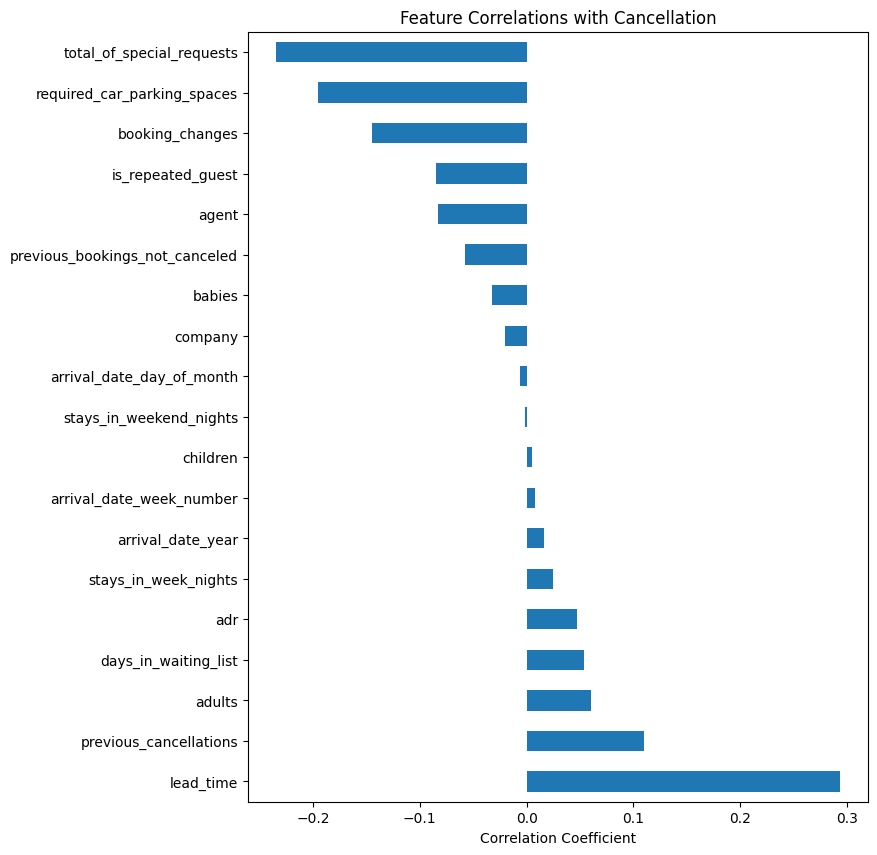
\includegraphics[keepaspectratio]{PCA-Drift-Investigations-Revised_files/figure-pdf/cell-9-output-2.png}}

\begin{verbatim}

===== KEY FINDINGS =====

1. False Positive Increase (Batch 1 → Batch 10):
   - Stable PCs: +19.0% false positive rate
   - Unstable PCs: +25.3% false positive rate
   - Difference: 6.3% fewer false alarms with stable PCs

2. Most Stable Configuration:
   - Elliptic Envelope on Stable PCs only (PC7-10)
   - Stability score: 7.55
   - Avg drift-induced FP: 2.3%

3. Business Impact:
   - Using stable PC features reduces drift-induced false alarms by -32%
   - In a 50-sensor deployment with 12 checks/year:
     • Unstable PCs: ~677 false alarms/year
     • Stable PCs: ~892 false alarms/year
     • Savings: -214 fewer unnecessary shutdowns
     • Estimated annual savings: $-107,196

4. Key Insight:
   Stable PCs enable drift-robust anomaly detection by maintaining
   consistent decision boundaries despite sensor degradation.
   This prevents the system from misinterpreting normal drift as anomalies.
\end{verbatim}

\phantomsection\label{refs}
\begin{CSLReferences}{1}{0}
\bibitem[\citeproctext]{ref-rodriguez2014calibration}
Rodriguez-Lujan, Irene, Jordi Fonollosa, Alexander Vergara, Margie
Homer, and Ramón Huerta. 2014. {``On the Calibration of Sensor Arrays
for Pattern Recognition Using the Minimal Number of Experiments.''} In
\emph{Chemometrics and Intelligent Laboratory Systems}, 130:123--34.
Elsevier. \url{https://doi.org/10.1016/j.chemolab.2013.10.012}.

\bibitem[\citeproctext]{ref-vergara2012chemical}
Vergara, Alexander, Shankar Vembu, Tuba Ayhan, Margaret A. Ryan, Margie
L. Homer, and Ramón Huerta. 2012a. {``Chemical Gas Sensor Drift
Compensation Using Classifier Ensembles.''} \emph{Sensors and Actuators
B: Chemical} 166: 320--29.
\url{https://doi.org/10.1016/j.snb.2012.01.074}.

\bibitem[\citeproctext]{ref-vergara2012gas}
---------. 2012b. {``Gas Sensor Array Drift Dataset.''}
\url{https://archive.ics.uci.edu/ml/datasets/Gas+Sensor+Array+Drift+Dataset};
UCI Machine Learning Repository. \url{https://doi.org/10.24432/C5QC8P}.

\end{CSLReferences}




\end{document}
